\documentclass[12pt,oneside,openany,a4paper,%..... Layout
               afrikaans, english,%.............. Global language selection
               ]{memoir}
\usepackage{graphics}
\usepackage{epstopdf}
\usepackage{amsmath,bm}
\usepackage{tikz}
\usepackage{tikz-dimline}
\usepackage{tikz-timing}[]
\usepackage[siunitx]{circuitikz}
\usetikzlibrary{circuits.logic.US} % TiKZ Library for US Logic Circuits.
\usetikzlibrary{calc,arrows,shapes,shadows,matrix,positioning}
\usepackage{siunitx}

 \usepackage[masters-t,%.......................... Master thesis
             goldenblock,%........................ A5 type block (or a5block or wide)
            ]{usthesis}%.......................... US thesis style with memoir

%
% PLEASE read the USthesis documentation for the class options
% and how to set line and paragraph spacing
%

%==== Language setup ================================================
 \usepackage[latin1]{inputenc}%................... Recognizes �, �, etc
 \usepackage{babel}%.............................. Language setup

%==== Math setup ====================================================
 \usepackage{amsmath,bm}%............................ Advanced math (before fonts)
 %\usepackage{amssymb}%............................ AMS Symbol fonts

%==== Font setup (default is Computer Modern) =======================
 \usepackage[T1]{fontenc}%........................ Type 1 fonts
 %\usepackage{fourier}
 \usepackage{textcomp}%........................... Additional text character
 \usepackage{bm}%................................. Bold math symbols (after fonts)

%==== Ref's, Bib's and Nomencl ======================================
 \usepackage{usnomencl}%.......................... List of symbols (in usthesis pack)
 \usepackage{usbib}%.............................. Bibliography    (in usthesis pack)
    \bibliographystyle{usmeg-a}
    \renewcommand\bibfont{\small}

    %% For usmeg-a, the bib is a list of references. If you
    %% are using usmeg-n comment out the following lines
    \addto{\captionsafrikaans}{\renewcommand{\bibname}{Lys van Verwysings}}
    \addto{\captionsenglish}{\renewcommand{\bibname}{List of References}}

%==== Graphics and Color ============================================
\usepackage{graphicx}%........................... Graphicx loaded in usthesis
\usepackage{color}%.............................. Color setup
\usepackage{eso-pic}%............................ Shipout commands for watermark
    \newcommand*{\WaterMark}[2][0.15\paperwidth]{%
        \AddToShipoutPicture*{\AtTextCenter{%
                \parbox[c]{0pt}{\makebox[0pt][c]{%
                    \includegraphics[width=#1]{#2}}}}}}

%==== Local Defs ====================================================
\makeatletter

%
% Please insert user defined commands here
% and NOT in the document itself!
%

\makeatother

%==== TITLE PAGE ====================================================
\title{\bfseries
       \AorE{%-- Afrikaans ------------------------------------------
             Die Terugvoer Beheer van 'n Robotiese Gimnas\\[1ex]
             \normalfont\small\itshape
             (``The Feedback Control of a Robotic Gymnast'')
            }{%-- English -------------------------------------------
             The Feedback Control of a Robotic Gymnast
            }}

\author{H.\ Kotz�}{Henry Kotz�}

\degree{\AorE{BIng (Megatronika)}{BEng (Mechatronics)}}
       {\AorE{Magister in Ingenieurswese (Meganiese)}
             {Master of Engineering (Mechanical)}}

\address{\AorE{%-- Afrikaans ----------------------------------------
        Departement Meganiese en Megatroniese Ingenieurswese,\\
        Universiteit van Stellenbosch,\\
        Privaatsak X1, Matieland 7602, Suid Afrika.%
             }{%-- English ------------------------------------------
        Department of Mechanical and Mechatronic Engineering,\\
        University of Stellenbosch,\\
        Private Bag X1, Matieland 7602, South Africa.
             }}

\faculty{\AorE{Fakulteit Ingenieurswese}%
              {Faculty of Engineering}}

\supervisor{Dr.\ J.A.A \ Engelbrecht }
\cosupervisor{}

\setdate{10}{2018}

%\SetSponsor{The financial assistance of the National Research Foundation (NRF)
%    towards this research is hereby acknowledged. Opinions expressed and
%    conclusions arrived at, are those of the author and are not necessarily to
%    be attributed to the NRF.}


%====================================================================
%     MAIN DOCUMENT
%====================================================================
\maxsecnumdepth{subsubsection}
\maxtocdepth{section}

\begin{document}

%==== Front matter ==================================================
 \frontmatter
 \WaterMark{UScrest-WM}
 \TitlePage

 \DeclarationDate{2018/10/27}
 \DeclarationPage

 \begin{abstract}[english]%===================================================
In this report a design method for the swinging and balancing  of the underactuated robotic gymnast was researched, simulated and tested on a physical model. The electronic, mechanical and software designs are discussed to show how the physical model was constructed, controllers implemented and data acquired.
\end{abstract}


\begin{abstract}[afrikaans]%=================================================
In die projek word die swaaiende en balanseering beheerwette vir 'n robotiese gimnas genavors, ontwerp en getoets op 'n fisiese model. Die eletroniese, meganiese en sagteware ontwerpe word bespreek om ten einde te wys hoe die fisiese model, beheerders en so voort geimplementeer en getoets is.
\end{abstract}


\chapter{Acknowledgements}%==================================================

I would like to express my sincere gratitude to the following people
and organisations.\\

Dr. Japie Engelbrecht for supervising the project throughout the year. He provided critical feedback on progress, guided me in the correct direction and was a voice of reason throughout the project.\\

The Electrical and Electronic Department for allowing the use of their equipment and facilities. They allowed me to work with confidence ensuring the facilities and equipment are maintained with no interruption to my work.\\

Mr$.$ Croukamp, Mr$.$ van Eenden and Mr$.$ Lecholo for assisting me with the mechanical and electronic designs. The atmosphere in the manufacturing labotorium was always welcoming.\\

The group of final year student working together in the 4th floor labs. You all made the experience more worthwhile and encouraged me through  difficult times. 




\chapter{Dedications}%=======================================================
 \vfill
 \begin{Afr}
 \begin{center}\itshape
    Hierdie verslag word opgedra aan my ouers wat my ondersteun het tydens die 4 jaar om die graad van ingenieurswese te ontvang en die Here vir sy genade. 
 \end{center}
 \end{Afr}
 \vfill
 \clearpage

%============================================================================
\endinput


 \tableofcontents
 \clearpage

 \setcounter{lofdepth}{2}
 \listoffigures
 \clearpage

 \listoftables
 \clearpage

 \chapter{Nomenclature}

\begin{Nomencl}
 \NomGroup{Constants}%-----------------------------------------------
   \item[$\mathrm{g} = $] $\mathrm{9.81\,m/s^2}$

 \NomGroup{Variables}%-----------------------------------------------
 	\item[$I$]         \UnitLine{Inertia                }{kg{\cdot}m^2}
 	\item[$m$]         \UnitLine{mass                }{kg}
 	\item[$l$]         \UnitLine{Lenght                }{m}
	\item[$L$]         \UnitLine{Lenght                }{m}
  	\item[$R$]			\UnitLine{Reaction Force}		{N}
  	\item[$T$]      	\UnitLine{Torque                    }{N{\cdot}m}
  	\item[$F$]      	\UnitLine{Force                    }{N}
   	\item[$x$]         	\UnitLine{Coordinate                }{m}
   	\item[$\ddot{x}$]  	\UnitLine{Acceleration              }{m/s^2}\\
   	\item[$\theta$]    	\UnitLine{Rotation angle            }{rad}
   	\item[$\phi$]    	\UnitLine{Rotation angle            }{rad}
   	\item[$\dot{\theta}$]    	\UnitLine{Angular velocity            }{rad/s}
   	\item[$\dot{\phi}$]    	\UnitLine{Angular velocity            }{rad/s}
   	\item[$\ddot{\theta}$]    	\UnitLine{Angular acceleration            }{rad/s^2}
   	\item[$\ddot{\phi}$]    	\UnitLine{Angular acceleration            }{rad/s^2}
   	\item[$\zeta$]     	\UnitLine{Damping Coefficient        }{1}
   	\item[$t$]      	\UnitLine{Time                    }{s}
   	\item[$\tau$]      	\UnitLine{Torque                    }{N{\cdot}m}
   	\item[$J$]      	\UnitLine{Polar second moment of area                    }{m^4}
   	
   	

 \NomGroup{Vectors}%-------------------------------------
   \item[$\vec{q}$] Angular position vector
   \item[$\vec{\dot{q}}$] Angular velocity vector
   \item[$\vec{\ddot{q}}$] Angular acceleration vector

 \NomGroup{Subscripts}%----------------------------------------------
   \item[$a$] 			Unactuated Pendulum
   \item[$b$]          	Actuated Pendulum
   \item[$1$]          	Unactuated Pendulum center of mass
   \item[$2$]          	Actuated Pendulum center of mass
\end{Nomencl}



\endinput


%==== Main document =================================================
\mainmatter
   \setsecnumdepth{subsubsection}
%   \numberwithin{equation}{section}
%   \numberwithin{figure}{chapter}
%   \numberwithin{table}{chapter}

\chapter{Introduction}
\label{chp:introduction}


%%%%%%%%%%%%%%%%%%%%%%%%%%%%%%%%%%%%%%%%%%%%%%%%%%%%%%%%%%%%%%%%%%%%%%%
\section{Problem Statement}

In this report a feedback control system for a robotic gymnast that is able to swing from the "hanging" position to the "handstand" position will be designed, implemented and verified. Feedback control loops must be designed that use the "legs" of the gymnast to swing the "body" of the gymnast from the "hanging" position to a "handstand" position and then balance the gymnast on top of the horizontal bar. A mathematical model for the dynamics of the swinging robotic gymnast system must be derived or sourced from literature. The dynamics are analysed to propose an appropriate feedback control architecture that actuates the "legs" of the gymnast using feedback from sensors that measure the swinging motion of the gymnast on a horizontal bar. A practical demonstrator must be constructed and the correct operation must be demonstrated.\\

\section{The Robotic Gymnast System}
\begin{figure}[h]
	\centering
	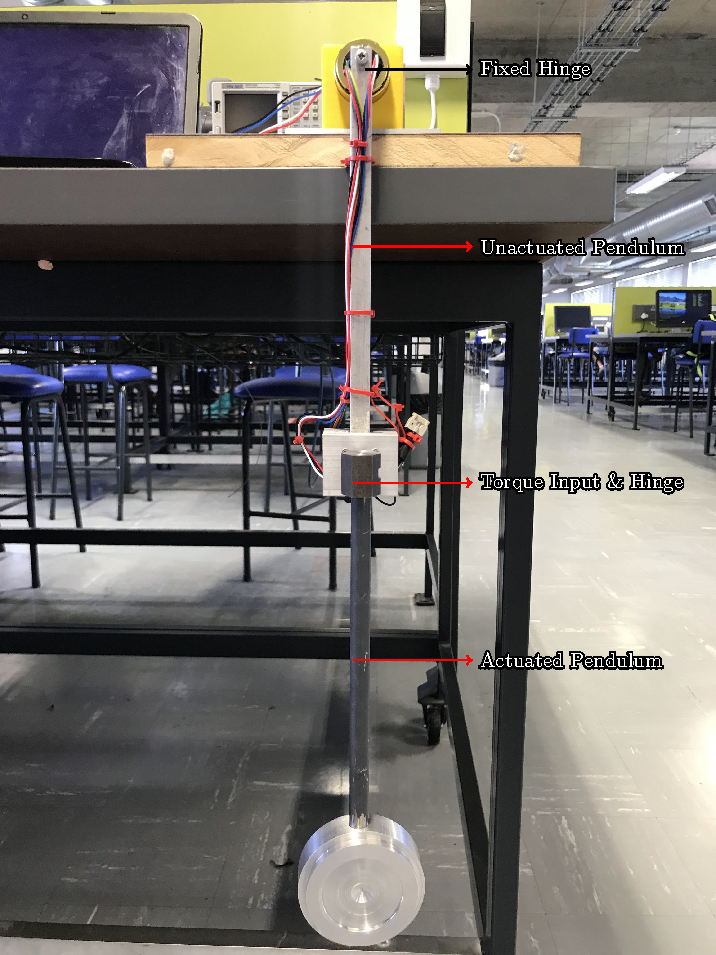
\includegraphics{./figs/overview/overview.pdf}
	\caption{Overview of the Robotic Gymnast System}
	\label{fig:overview}
\end{figure}

Figure \ref{fig:overview} provides an overview of the system to create a mental picture for the variables and concepts used throughout the report. There are 2 pendulums that are attach together with a hinge. At this hinge there is a torque being applied by a motor to the actuated pendulum. The entire system rotates around the fixed hinge at the top to which the unactuated pendulum is connected. The system is describe using two independent parameters, $\theta$ and $\phi$ which describes the entire system.\\

The goal is to use the feedback of the independent parameters to apply a torque to the actuated pendulum to swing the gymnast from the hanging position and balance in the inverted position. This is accomplished by designing a microcontroller to interface with sensors to provide information about the independent parameters and implement the control laws for the balancing and swinging in software.\\


\section{Literature Study}
\label{sec:literature_study}
% WHAT you are going to present in this chapter/section
% WHY you are presenting it, and
% HOW you are going to present it
\begin{comment}
	Previous approaches used to control an underactuated system is to use the intrinsic dynamics of the system to attain the desired behaviour \citep{tedrake}. This leads to the approach to exploit the dynamics of the system by using the 'legs' of gymnast to swing.\\
\end{comment}	

A literature study was performed to survey different physical implementations of the system, different approaches to modelling the dynamics, different physical implementations of the system, and different techniques to perform the feedback control to perform the swing-up and the balancing of the robotic gymnast.\\

Previous attempts to swing up and balance the robotic gymnast used two separate controllers. The first controller is responsible for swinging the robotic gymnast from the hanging position up towards the inverted position. When the swing-up controller brought the gymnast near the inverted position, a new controller is used balance the gymnast. The different types of swing up and balancing controllers used by previous researchers are summarised below, followed by a decision on the approaches selected for this project..\\

\citet{spong_swingup} implemented the swing-up controller by using partial feedback linearisation which results in a linear response from either the \textit{actuated} or \textit{unactuated} pendulum. Using \textit{non-collocated} linearisation he was able to control the \textit{unactuated} pendulum to follow a desired trajectory and used the phase portrait of the zero dynamics of the system to show that the closed-loop system will converge to the inverted equilibrium position. \citeauthor{spong_swingup} also demonstrated how the swing-up can be achieved by using \textit{collocated} linearisation which linearises the response of the \textit{actuated} pendulum. This allows the actuated pendulum to follow a desired trajectory and \citeauthor{spong_swingup} provides a energy-based trajectory that increases the energy in the system. Once the both swing up controller brings the system to the inverted balancing position, the feedback control system switches over to a linear quadratic regulator (LQR) to balance the system.\\

\citet{Brown1997} provided two manually tuned nonlinear controllers for the balancing of the robotic gymnast and tested and compared them against a designed LQR controller. The two nonlinear controller were a direct fuzzy controller (DFC) and a fuzzy model reference learning controller (FMRLC). The gains for the DFC controller were based on the gains of the LQR controller. The DFC controller was implemented and successfully balanced the gymnast. However the LQR controller provided smoother state trajectories and smaller control input. The FMRLC uses no explicit dynamical reference model and instead the outputs of the plant using normalising gains are directly fed into the second fuzzy system. The FMRLC controller was a significant improvement on the DFC, but yet again did not perform as well as the LQR controller.\\


\citeauthor{Brown1997} also attempted to swing the acrobat to the inverted balancing position using the energy based trajectory proposed by \citeauthor{spong_swingup}, but without the partial linearisation feedback. \citeauthor{Brown1997} were able to swing and balance the acrobat using this approach,but their approach resulted in larger input signals that were not as smooth as the input signals when using partial feedback linearisation.\\



In most of the literature, the mathematical model of the robotic gymnast is derived using the Euler-Lagrangian equation. This approach is used because the mechanical energy in the system is easily identified. \citet{derivation_controlPlaner} and \citet{tedrake} both derived the simplified mathematical models for the robotic gymnast using point mass approximations. \\

Based on the literature study, it was decided to perform the swing up control using partial feedback linearisation and an energy-based reference trajectory, and to perform the balancing control using a linear full state feedback controller.


\begin{comment}


The ordinary differential equations (ODE's) describing a system can be arranged as a set of linear differential equations. Describing a system in such a way is known as the State Space design approach, where the solution is the trajectory of the chosen state variables.\cite{textbook}

These ODE's are required to be written as vectors in the state-variable form seen in equation (\ref{eq:statespace1}) and (\ref{eq:statespace2})
\begin{equation} \label{eq:statespace1}
\centering
\boldsymbol{\dot{x}} = \boldsymbol{A}\boldsymbol{x} + \boldsymbol{B}u
\end{equation}
\begin{equation} \label{eq:statespace2}
\centering
\boldsymbol{y} = \boldsymbol{C}\boldsymbol{x} + Du
\end{equation}
The \textit{n}th-column vector $\boldsymbol{x}$ is called the state of the system for a \textit{n}th-order system. The \textbf{A} matrix is the system matrix, containing \textit{n}$\times$\textit{n} elements and the input matrix is the \textit{n}$\times 1$ \textbf{B} matrix. \textbf{C} is a $1\times$\textit{n} row matrix called the output matrix and the scalar D is known as the direct transmission term \cite{textbook}.

A system parameter of great interest to control engineers are the poles of the system. It provides the characteristic response of the system starting at a initial condition with no forcing function. These poles,\textbf{s}, are the natural frequencies of the system and the state space representation allow these poles to be easy identified. The poles are the solution to the eigenvalue problem of the \textbf{A} matrix shown in equation (\ref{eq:statespace_eigen}) \cite{textbook}.
\begin{equation} \label{eq:statespace_eigen}
\centering
\text{det}(s\boldsymbol{I} - \boldsymbol{A}) = 0
\end{equation}

The poles of the system can be assigned new positions to satisfy dynamic response specification by introducing feedback. The feedback is a linear combination of the state variables $\boldsymbol{x}$ resulting in the input of the system $u$ to be transformed as seen in equation (\ref{eq:feedbackgain}) and represented in Figure \ref{fig:linearSys}. Substituting equation (\ref{eq:feedbackgain}) into (\ref{eq:statespace1}) the characteristic equation is now describe as (\ref{eq:closedSysFeedback}). The corresponding characteristic equation is: $$\alpha_{s}=(s-s_{1})(s-s_{2})\ldots(s-s_{n}) $$ This shows by selecting the correct gain matrix \textbf{K} the poles of the system can be moved to a desired position.
\begin{equation} \label{eq:feedbackgain}
\centering
u = -\boldsymbol{K}\boldsymbol{x}
\end{equation}

\begin{figure}
	\centering
	% System Combination
% Harish K Krishnamurthy <www.ece.neu.edu/~hkashyap/>
\documentclass{article}

\usepackage{tikz}
\usetikzlibrary{shapes,arrows,shadows}
\usepackage{amsmath,bm,times}
\newcommand{\mx}[1]{\mathbf{\bm{#1}}} % Matrix command
\newcommand{\vc}[1]{\mathbf{\bm{#1}}} % Vector command

\begin{document}
	% Define the layers to draw the diagram
	\pgfdeclarelayer{background}
	\pgfdeclarelayer{foreground}
	\pgfsetlayers{background,main,foreground}
	
	% Define block styles used later
	
	\tikzstyle{sensor}=[draw, fill=blue!20, text width=5em, 
	text centered, minimum height=2.5em,drop shadow]
	\tikzstyle{ann} = [above, text width=5em, text centered]
	\tikzstyle{wa} = [sensor, text width=10em, fill=red!20, 
	minimum height=6em, rounded corners, drop shadow]
	\tikzstyle{sc} = [sensor, text width=13em, fill=red!20, 
	minimum height=10em, rounded corners, drop shadow]
	
	% Define distances for bordering
	\def\blockdist{2.3}
	\def\edgedist{2.5}
	
	\begin{tikzpicture}
	\node (wa) [sensor]  {$\boldsymbol{\dot{x}}= \boldsymbol{A}\boldsymbol{x}+\boldsymbol{B}$};
	\path (wa.south)+(0,-1) node (feedback) [sensor] {$u = -\boldsymbol{K}\boldsymbol{x}$};
	
	\path (wa.east)+(\blockdist/1.5,0) node (C) [sensor] {$\boldsymbol{C}$};
	\path (C.east)+(\blockdist/1.5,0) node (Y) [sensor] {$\boldsymbol{y}$};
	
	
	\path [draw, ->,thick] (wa.east) -- node [above] {} 
	(C.west);
	
	\path [draw, ->,thick] (C.south) |- node [above] {} 
	(feedback.east);
	
	\path [draw, ->,thick] (C.east) -- (Y.west);
	
	\path [draw, ->,thick] (feedback.west) -| ([xshift=-1cm]wa.west) -- (wa.west) {};
	
	%\path [draw, ->,] (C.east) -- node [above] {} 
	%	(Y.west);
	
	%\path (wa.south) +(0,-\blockdist) node (asrs) {System Combination - Training};
	
	%\begin{pgfonlayer}{background}
	%   \path (asr1.west |- asr1.north)+(-0.5,0.3) node (a) {};
	%  \path (wa.south -| wa.east)+(+0.5,-0.3) node (b) {};
	% \path (C.east |- asrs.east)+(+0.5,-0.5) node (c) {};
	
	%\path[fill=yellow!20,rounded corners, draw=black!50, dashed]
	%   (a) rectangle (c);           
	% \path (asr1.north west)+(-0.2,0.2) node (a) {};
	
	%\end{pgfonlayer}
	
	\end{tikzpicture}
	
\end{document}}
	\caption{State Space Representation with Feedback Gain}
	\label{fig:linearSys}
\end{figure}

\begin{equation} \label{eq:closedSysFeedback}
\centering
\text{det}[s\boldsymbol{I}-(\boldsymbol{A}-\boldsymbol{B}\boldsymbol{K})] = 0
\end{equation}

The classical approach to controlling a system is by implementing a controller which reacts on the error of the desired state and the current state. These controllers are more commonly known as PID-controllers where the controller equation is shown in (\ref{eq:PID}).

\begin{equation} \label{eq:PID}
\centering
u(t) = K[ e(t)+K_{I}\int_{0}^{t}e(\tau)d\tau +K_{D}\frac{de(t)}{dt}]
\end{equation}

Each term represent an effect it has on the system response when the PID-controller is implemented shown in Figure \ref{fig:PIDcontroller}. If the system or plant is assumed to be a second-order differential equation represented by:
\begin{equation} \label{eq:PID_system}
\centering
\dddot{q}+(2\zeta\omega_{n}+K_{D})\ddot{q}+(\omega_{n}^2+K_{P})\dot{q}+K_{I} = 0
\end{equation}

From equation (7) it is visible that by tuning the PID constants the response of the system can controlled.
\end{comment}


\section{System Overview}
\label{sec:system_overview}
%WHAT you are going to present in this chapter/section
%WHY you are presenting it, and
%HOW you are going to present it
\begin{figure}[h]
	\centering
	\newcommand{\mx}[1]{\mathbf{\bm{#1}}} % Matrix command
\newcommand{\vc}[1]{\mathbf{\bm{#1}}} % Vector command


% Define the layers to draw the diagram
\pgfdeclarelayer{background}
\pgfdeclarelayer{foreground}
\pgfsetlayers{background,main,foreground}

% Define block styles used later

\tikzstyle{sensor}=[draw, fill=red!20, text width=5em, 
text centered, minimum height=2.5em,drop shadow,rounded corners]
\tikzstyle{ann} = [above, text width=5em, text centered]
\tikzstyle{wa} = [sensor, text width=10em, fill=red!20, 
minimum height=6em, rounded corners, drop shadow]
\tikzstyle{sc} = [sensor, text width=13em, fill=red!20, 
minimum height=10em, rounded corners, drop shadow]

% Define distances for bordering
\def\blockdist{2.3}
\def\edgedist{2.5}

\begin{tikzpicture}[scale=1.2]
\centering
\node (wa) [wa]  {\textbf{Electronic Design} \\ PCB \\ Signal Conditioning};
\path (wa.west)+(-\blockdist,0) node (asr1) [wa] {\textbf{External Computer} \\ Controller \\ Data Aquisition };
\path (wa.east)+(\blockdist,0) node (vote) [wa] {\textbf{Mechanical Design} \\ State variables \\ };
\path (wa.north)+(0,\blockdist/2) node (pow) [sensor] {\textbf{External Power}};
\path (asr1.north)+(0,\blockdist/2) node (human) [sensor] {\textbf{Human Input} \\ };


\path [draw, <->,thick] (asr1.east) -- node [above] {} 
(wa.west) ;

\path [draw, <->,thick] (wa.east) -- node [above] {} 
(vote.west);

\path [draw, <->,thick] (human.south) -- node [above] {} 
(asr1.north);   

\path [draw,thick, ->] (pow.south) -- node [above] {} 
(wa.north);   


\path (wa.south) +(0,-\blockdist/2) node (asrs) {};
 \path (wa.south)+(0,-\blockdist/5) node (meep) {System Boundary};


\begin{pgfonlayer}{background}
\path (asr1.west |- asr1.north)+(-0.5,0.3) node (a) {};
\path (wa.south -| wa.east)+(+0.5,-0.3) node (b) {};
\path (vote.east |- asrs.east)+(+0.5,0.5) node (c) {};

\path[fill=yellow!20,rounded corners, draw=black!50, dashed]
(a) rectangle (c);           
\path (asr1.north west)+(-0.2,0.2) node (a) {};

\end{pgfonlayer}

\end{tikzpicture}
	\caption{System Overview of the Feedback Control of Robotic Gymnast}
	\label{fig:system_overview}
\end{figure}


Figure \ref{fig:system_overview}  provides an overview of the system that was developed in this project , and shows the individual subsystems with their internal and external interfaces. The individual subsystems could be developed separately with well-defined interfaces to one another. A brief overview of each subsystem is presented here.\\

The external computer executes the feedback control laws that perform the swing up and balancing, and supplies the commands for the motor actuator based on sensor feedback from the angle sensors for both the actuated and the non-actuated pendulums. This allows for the verification of system parameters, debugging and experimental tests.\\

The electronic hardware acts as the interface between external computer and the robotic gymnast mechanical hardware. The external computer communicates with the electronic hardware using serial communications to send commands and to receive data. The electronic hardware interfaces directly with the motor actuator using a motor driver, and interfaces with the angle sensors using digital and analog interfaces. The electronic hardware is implemented on a printed circuit board (PCB).\\

A mechanical prototype system was designed and constructed. The mechanical system consists of the mechanical structure of the robotic gymnast, the motor actuator, and the angle sensors for the two pendulum links (unactuated and actuated). The motor actuator is controlled by the electronic hardware based on commands provided by the external computer, and the two angle sensors are read by the electronic hardware, and their measurements are transmitted back to the external computer.\\

The external interfaces to the system include the power supplied to the system and the input commands provided by the user.

\section{Project Execution}
%WHAT you are going to present in this chapter/section
%WHY you are presenting it, and
%HOW you are going to present it
% write as if i already happened

The project was executed in a sequence of steps in order to achieve the results as presented in the report. It is presented to provide the reader with an understanding of how the individual subsystems were developed individually and eventual	ly integrated into the full system.\\
 
First the mathematical model of the system was derived by using the appropriate approach. The derived mathematical model was then implemented on a simulation program where the dynamics of the system was verified and inspected.\\

Following the successful implementation of the mathematical model the various controllers were designed and implemented on the simulation program. The behaviour of the simulated responses were inspected and analysed.\\

The simulation provided the specification for the mechanical design to commence and created the physical model that provided an acceptable representation of the mathematical model.\\

During manufacturing of the mechanical design the electronic design started. Conceptual designs were created capable of meeting the requirements and the selected design was manufactured. The electronic design was then tested to ensure it performs as designed with the opportunity to create revisions.\\

Following the successful testing of the electronic design, the programming of the microcontroller and external computer started. This included the programming of the controller, data acquisition system and the conversions of the sampled data.\\

Once the microcontroller could provide the external computer with system state information, the system identification tests occurred to determine the various system parameters. These new system parameters were used in the simulation program to update the existing controllers and verify the responses in simulation.\\

The updated controllers were then implemented onto the external computer for the system experiments to start. From these system experiments the response of the experiments were compared to those of the simulation.\\

The report was written throughout the sequence of steps mentioned above and was completed and reviewed at the end.


\section{Report Outline}
%WHAT you are going to present in this chapter/section
%WHY you are presenting it, and
%HOW you are going to present it

A brief overview of each chapter in the report is provided here. It acts as a primer for the reader and the identification of sections that may interest the reader more.\\

Chapter 2 explains the system concepts that is refered to throughout the report. It contains the mathematical derivation of the robotic gymnast and the simulated model. The system parameters with system identification tests are shown and demonstrates the simulated model is an acceptable representation of the physical model.\\

Chapter 3 describes the controller architecture to the swinging and balancing of the robotic gymnast. The specification for the controllers and the simulated responses of the controller are provided.\\

Chapter 4 contains the designs of the mechanical and electronic systems of the project. The various components used in the designs are discussed and explained.\\

Chapter 5 describes the software implemented to provide the report with these results. It explains the architecture of the software and the various functions implemented.\\

Chapter 6 provides the practical results of the controllers explained in chapter 3 and hypothesise unexpected behaviour in the experiments.\\

Chapter 7 concludes the report with a summary of the report and recommendation for future endeavours on the Feedback Control of a Robotic Gymnast. 

 

\chapter{Conceptualisation and Modelling}
\label{chp2:concept_model}
This chapter presents variable names and use of terminology for concepts that is used throughout the report. The approach used to derive the dynamics of the robotic gymnast is discussed and how a simulation program was used to present the dynamics appropriately. The system identification tests are presented to show how the system characteristics were determined and that the simulated model describes the physical model accurately. The terminology for concepts are presented first, followed by the derivation of the dynamics of the robotic gymnast. A discussion of the simulated model is then presented and the chapter concludes with the system identification test and the verification of the simulated model.

\section{System Concepts}
%WHAT you are going to present in this chapter/section
%WHY you are presenting it, and
%HOW you are going to present it
The double pendulum is a underactuated system which is defined as a system where the input to the system cannot command all of the state variables an instantaneous acceleration \citep{tedrake}. This is due to the control input only actuating the lower pendulum and the energy in the lower pendulum must be transferred to the upper pendulum to initiate an acceleration. \\

The robotic gymnast is described as a double pendulum consisting out of an actuated- and unactuated pendulum as seen in Figure \ref{fig:doublePen}. The position of the unactuated pendulum is described by the angle $\theta$ whereas the actuated pendulum is described by $\phi$ relative to $\theta$. The angle's $\theta$ and $\phi$ are the independent parameters that describe the entire system.\\

There are two position of interest where the system contain special characteristics. These 2 positions are the stable- and unstable equilibrium positions. In the stable position the system is at rest hanging downwards where both $\theta$ and $\phi = \SI{0}{\radian}$. The unstable equilibrium position is where $\theta=\SI{2\pi}{\radian}$ and $\phi = \SI{0}{rad}$ resulting in the robotic gymnast balancing in the inverted position.\\


\section{Mathematical Model}
\label{sec:mathematical_model}
%WHAT you are going to present in this chapter/section
%WHY you are presenting it, and
%HOW you are going to present it
\begin{figure}[h]
	\centering
	
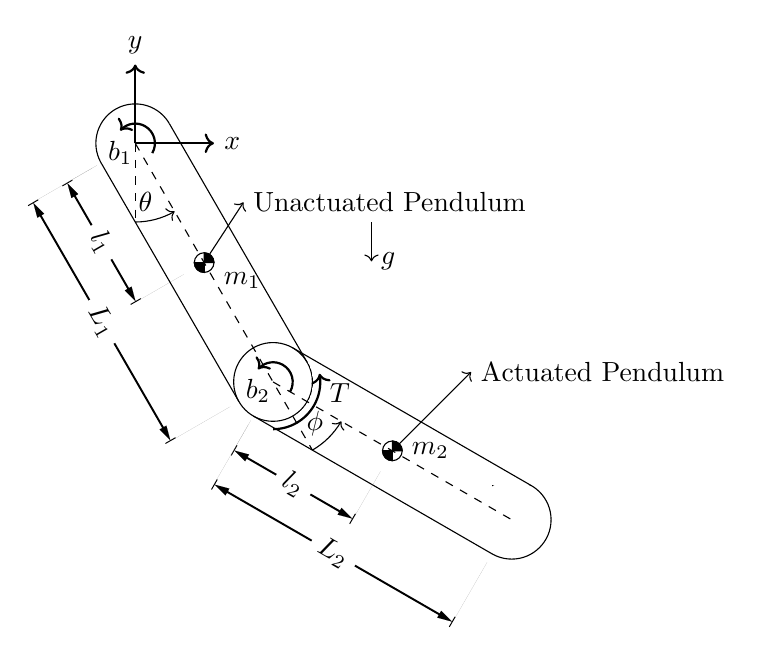
\begin{tikzpicture}[scale=0.5]

\begin{scope}
\clip [rotate=30] (-2,0) rectangle (2,2);
\draw (0,0) circle [radius=1cm];
\end{scope}

\coordinate (O) at (0,0) ;
% Second cirle middle point
\coordinate (A) at (3.5,-6.06217); 
\coordinate (B) at (3.5+6.06217,-6.06217-3.5); 
	% Lenght of pendulums are 7cm

	% Axis for underactuated Pendulum
	\draw[->,thick] (0,0) -- (2,0) node[anchor=west] {$x$};
	\draw[->,thick] (0,0) -- (0,2) node[anchor=south] {$y$};
	\draw[dashed] (0,0) -- (0,-2);
	
	%%%%%%%%%%%%%%%%%%%%%%%%%%%%%%%%%%%%%%%%%%%%%%%%%%%%%%%%%%%%%%%%%%%%%%%%%%%%%%
							%% Theta %%
	\begin{scope}
		\draw[->] (0,-2) arc (270:300:2);
		\draw (280:1.5) node {$\theta$};
	\end{scope}
	%%%%%%%%%%%%%%%%%%%%%%%%%%%%%%%%%%%%%%%%%%%%%%%%%%%%%%%%%%%%%%%%%%%%%%%%%%%%%%
	
	%%%%%%%%%%%%%%%%%%%%%%%%%%%%%%%%%%%%%%%%%%%%%%%%%%%%%%%%%%%%%%%%%%%%%%%%%%%%%%
				%% Middle line for underactuated pendulum %%
	\draw[dashed] (0,0) -- (4.5,-7.79422);
	%%%%%%%%%%%%%%%%%%%%%%%%%%%%%%%%%%%%%%%%%%%%%%%%%%%%%%%%%%%%%%%%%%%%%%%%%%%%%%
	
		
	%%%%%%%%%%%%%%%%%%%%%%%%%%%%%%%%%%%%%%%%%%%%%%%%%%%%%%%%%%%%%%%%%%%%%%%%%%%%%%
					%% Dimensions of underactuated Pendulum %%
	\dimline[line style = {line width=0.7},extension start length=-0.25, extension end length=-0.4]{(-1.732,-1)}{(-1.732+1.75,-1-3.031)}{$l_{1}$}
	
	\dimline[line style = {line width=0.7},extension start length=-0.25, extension end length=-0.25]{(-2.598,-1.5)}{(-2.598+3.5,-1.5-6.06217)}{$L_{1}$}
	
	%%%%%%%%%%%%%%%%%%%%%%%%%%%%%%%%%%%%%%%%%%%%%%%%%%%%%%%%%%%%%%%%%%%%%%%%%%%%%%

	%Long lines for underactuated pendulum
	\draw (0.8660,0.5) -- (0.866+3.5,0.5-6.06217);
	\draw (-0.8660,-0.5) -- (-0.866+3.5,-0.5-6.06217);	
	
	
	
	%%%%%%%%%%%%%%%%%%%%%%%%%%%%%%%%%%%%%%%%%%%%%%%%%%%%%%%%%%%%%%%%%%%%%%%%%%%%%%
					%% Middle circle for both pendulums %%
	\begin{scope}
		%\clip [rotate=00] (0.866+3.5,0.5-6.06217+2) rectangle (-0.866+3.5-2,-0.5-6.06217);
	\clip (A) circle [radius=1.02];
	\draw (A) circle [radius=1cm];
	\end{scope}
	
	%\draw [rotate=00] (0.866+3.5,0.5-6.06217+2) rectangle (-0.866+3.5-2,-0.5-6.06217);
	
	%%%%%%%%%%%%%%%%%%%%%%%%%%%%%%%%%%%%%%%%%%%%%%%%%%%%%%%%%%%%%%%%%%%%%%%%%%%%%%
	% Axis for lower Pendulum
	%\draw[->,thick] (3.5,-6.06217) -- (6.5,-6.06217) node[anchor=west] {$x_{2}$};
	%\draw[->,thick] (3.5,-6.06217) -- (3.5,-3.06217) node[anchor=south] {$y_{2}$};
	%\draw[dashed] (3.5,-6.06217) -- (3.5,-8.56217);
	
	% Long lines for actuated pendulum
	\draw (3.5+0.5,-6.06217+0.86602) -- (3.5+0.5+6.06217,-6.06217+0.86602-3.5);
	\draw (3.5-0.5,-6.06217-0.86602) -- (3.5-0.5+6.06217,-6.06217-0.86602-3.5);
	
	%%%%%%%%%%%%%%%%%%%%%%%%%%%%%%%%%%%%%%%%%%%%%%%%%%%%%%%%%%%%%%%%%%%%%%%%%%%%%%
							%%  Phi %%
	\begin{scope}
	\draw[->] (4.5,-7.79422) arc (300:330:2);
	
	
	\draw (3.5,-6.06217)+ (315:1.5) node {$\phi$};
	\end{scope}
	%%%%%%%%%%%%%%%%%%%%%%%%%%%%%%%%%%%%%%%%%%%%%%%%%%%%%%%%%%%%%%%%%%%%%%%%%%%%%%
	
	%%%%%%%%%%%%%%%%%%%%%%%%%%%%%%%%%%%%%%%%%%%%%%%%%%%%%%%%%%%%%%%%%%%%%%%%%%%%%%
						%% Dimensions of actuated Pendulum %%
	\dimline[line style = {line width=0.7},extension start length=-0.25, extension end length=-0.4]{(2.5,-7.79421)}{(5.53108,-9.54422)}{$l_{2}$}
	
	\dimline[line style = {line width=0.7},extension start length=-0.25, extension end length=-0.25]{(2,-8.66028)}{(8.06217,-12.1602)}{$L_{2}$}
	
	%%%%%%%%%%%%%%%%%%%%%%%%%%%%%%%%%%%%%%%%%%%%%%%%%%%%%%%%%%%%%%%%%%%%%%%%%%%%%%

	
	%%%%%%%%%%%%%%%%%%%%%%%%%%%%%%%%%%%%%%%%%%%%%%%%%%%%%%%%%%%%%%%%%%%%%%%%%%%%%%
							%% Circle at the bottom %%
	\begin{scope}
	\clip [rotate=00] (3.5+0.5+6.06217+2,-6.06217+0.86602-3.5) rectangle ((3.5-0.5+6.06217,-6.06217-0.86602-3.5-2);
	\draw (B) circle [radius=1cm];
	\end{scope}
	%%%%%%%%%%%%%%%%%%%%%%%%%%%%%%%%%%%%%%%%%%%%%%%%%%%%%%%%%%%%%%%%%%%%%%%%%%%%%%

	
	%%%%%%%%%%%%%%%%%%%%%%%%%%%%%%%%%%%%%%%%%%%%%%%%%%%%%%%%%%%%%%%%%%%%%%%%%%%%%%
					%% Middle line for actuated pendulum %%
	\draw[dashed] (3.5,-6.06217)--(3.5+6.06217,-6.06217-3.5);
	%%%%%%%%%%%%%%%%%%%%%%%%%%%%%%%%%%%%%%%%%%%%%%%%%%%%%%%%%%%%%%%%%%%%%%%%%%%%%%
		
	%%%%%%%%%%%%%%%%%%%%%%%%%%%%%%%%%%%%%%%%%%%%%%%%%%%%%%%%%%%%%%%%%%%%%%%%%%%%%%
				%% Centroid symbol for underactuade pendulum %%
	\draw (1.75,-3.0310) circle [radius=0.25cm];
	\draw (1.75-0.25,-3.0310) -- (1.75+0.25,-3.0310)  node[below right]{$m_{1}$};`
	\draw (1.75,-3.0310+0.25) -- (1.75,-3.0310-0.25);
	\filldraw[fill=black,draw=black] (1.75,-3.0310) -- (1.75+0.25,-3.0310)
		arc[start angle = 0, end angle = 90, radius = 0.25] -- cycle;
		
	\filldraw[fill=black,draw=black] (1.75,-3.0310) -- (1.75-0.25,-3.0310)
	arc[start angle = 180, end angle = 270, radius = 0.25] -- cycle ;
	%%%%%%%%%%%%%%%%%%%%%%%%%%%%%%%%%%%%%%%%%%%%%%%%%%%%%%%%%%%%%%%%%%%%%%%%%%%%%%
	
	%%%%%%%%%%%%%%%%%%%%%%%%%%%%%%%%%%%%%%%%%%%%%%%%%%%%%%%%%%%%%%%%%%%%%%%%%%%%%%
				%% Centroid symbol for actuaded pendulum %%
	\draw (6.53108,-7.81217) circle [radius=0.25cm];
	\draw (6.53108-0.25,-7.81217) -- (6.53108+0.25,-7.81217)  node[right]{$m_{2}$};
	\draw (6.53108,-7.81217+0.25) -- (6.53108,-7.81217-0.25);
	\filldraw[fill=black,draw=black] (6.53108,-7.81217) -- (6.53108+0.25,-7.81217)
	arc[start angle = 0, end angle = 90, radius = 0.25] -- cycle;
	
	\filldraw[fill=black,draw=black] (6.53108,-7.81217) -- (6.53108-0.25,-7.81217)
	arc[start angle = 180, end angle = 270, radius = 0.25] -- cycle ;
	%%%%%%%%%%%%%%%%%%%%%%%%%%%%%%%%%%%%%%%%%%%%%%%%%%%%%%%%%%%%%%%%%%%%%%%%%%%%%%
	
	% Torque Input
	%\draw[->,thick] (3.5,-7.5) to [bend right] (5.25,-4.76314) node[right]{$T$}; 
	\draw[->,thick] (A) +(0,-1.2) arc (270:370:1.2) node[below right] {$T$};
	
	
	% Damping in bearings
	\draw[->,thick] (0.433,-0.25) arc (330:500:0.5) node[below] {$b_{1}$};
	
	% Damping between motor rotor and stator 
	\draw[->,thick] (A)+(0.433,-0.25) arc (330:500:0.5) node[below] {$b_{2}$};
	
	% Direction of gravity
	\draw[->] (6,-2)--(6,-3) node[right]{$g$};
	
	% Labels for pendulums
	\draw[->] (1.75,-3.0310)--(2.75,-1.5) node[right]{Unactuated Pendulum};
	\draw[->] (6.53108,-7.81217)--(8.53108,-5.81217) node[right]{Actuated Pendulum};
	
	
\end{tikzpicture}
	\caption{Free Body Diagram of the Double Pendulum}
	\label{fig:doublePen}
\end{figure}

The approach taken to derive the mathematical model of the robotic gymnast is presented in this section. It is presented to allow the reader to understand parameters used throughout the report and critical to the implementation of the swing-up controller. The swinging of the robotic gymnast consists of non-linear behaviour and is required to fully derive the dynamics of the system. The detailed mathematical derivations are available in Appendix \ref{sec:math_model}. A summary of the motivation and paradigm approach to the derivation is provided here.\\

 Figure \ref{fig:doublePen} shows the free body diagram of the robotic gymnast which was modelled as two pendulums connected together with a hinge. Each pendulum was modelled as having their mass distributed arbitrary along their axis. A torque is actuating the lower pendulum and friction was modelled as a function of the angular velocity.\\

The Euler-Lagrange equation shown in (\ref{eq:euler_lagrange_expanded}) was used to derive the dynamics of the system by analysing the energy of the system which is easily defined as the potential energy $T$ and the kinetic energy $V$ of the 2 pendulums.
 
\begin{equation} \label{eq:euler_lagrange_expanded}
\frac{d}{dt}\frac{\partial\mathcal{L}}{\partial\vec{\dot{q}}}-\frac{\partial\mathcal{L}}{ \vec{\partial q}} = 0
\end{equation}

\begin{equation} \label{eq:euler_lagrane}
\mathcal{L}=T-V
\end{equation}

Using the Euler-Lagrange equation leads to the condense equations shown in (\ref{eq:condense1}) and (\ref{eq:condense2}),
\begin{equation} \label{eq:condense1}
d_{11}\ddot{\theta}+d_{12}\ddot{\phi} + h_{1} + \psi_{1} = 0
\end{equation}
\begin{equation} \label{eq:condense2}
d_{21}\ddot{\theta} + d_{22}\ddot{\phi} + h_{2} + \psi_{2} = \tau
\end{equation}
where the coefficients are defined as
\begin{equation} \label{eq:d11}
d_{11} = I_{a} + I_{b} + m_{2}(L_{1}^2 + l_{2}^2+2L_{1}l_{2}\cos(\phi))
\end{equation}
\begin{equation} \label{eq:d12}
d_{12} = I_{b} +m_{2}(l_{2}^2 L_{1}l_{2}\cos(\phi))
\end{equation}
\begin{equation} \label{eq:h1}
h_{1} = -m_{2}L_{1}l_{2}\sin(\phi)\dot{\phi^2}-2m_{2}L_{1}l_{2}\sin(\phi)\dot{\phi}\dot{\theta}
\end{equation}
\begin{equation} \label{eq:psi1}
\psi_{1} = (m_{2}l_{1}+m_{2}L_{1})g\cos(\theta) + m_{2}l_{2}g\cos(\theta+\phi) + f_{c_{1}}
\end{equation}
\begin{equation} \label{eq:d21}
d_{21}= I_{b}+m_{2}(l_{2}^2+L_{1}l_{2}\cos(\phi))
\end{equation}
\begin{equation} \label{eq:d22}
d_{22}= I_{b}+ m_{2}l_{2}^2
\end{equation}
\begin{equation} \label{eq:h2}
h_{2}= m_{2}L_{1}l_{2}\sin(\phi)\dot{\theta^2}
\end{equation}
\begin{equation} \label{eq:psi2}
\psi_{2}= m_{2}l_{2}g\cos(\theta+\phi) + f_{c_{2}}
\end{equation}

The friction that develops in the pendulums are for now represented by the $f_{c_{1}}$ and $f_{c_{2}}$ terms and will be expanded in the system identification section.

\section{Simulation Model}
\label{sec:simulation_model}
	%WHAT you are going to present in this chapter/section
%WHY you are presenting it, and
%HOW you are going to present it

The mathematical model derived in the previous section was implemented in a simulation program so that the controllers can be tested in simulation. Simulating the model allows the designer to understand how system parameters influence the dynamics of the system and the verification of controllers implemented. It will be presented by discussing the non-linearities added to represent the physical model better.\\

Simulation of the robotic gymnast was done using \textit{MATLAB Simulink}. The differential equations shown in equation (\ref{eq:condense1}) and (\ref{eq:condense2}) were implemented using the \textit{MATLAB Function} box. It was required to write $\ddot{\phi}$ and $\ddot{\theta}$ as the subject in each of the \textit{MATLAB Function} box to allow MATLAB to simulate the model.\\

Non-linear behaviour introduced by sensors and components were added such as saturation of the motor torque, gearbox backlash and quantisation of sensory data. These non-linearities were implemented to allow the simulation to be an acceptable representation of the physical system. The Simulink model used for simulation is shown in Figure \ref{fig:sim_nonlinearfeedback}.

\begin{figure}[h]
	\centering
	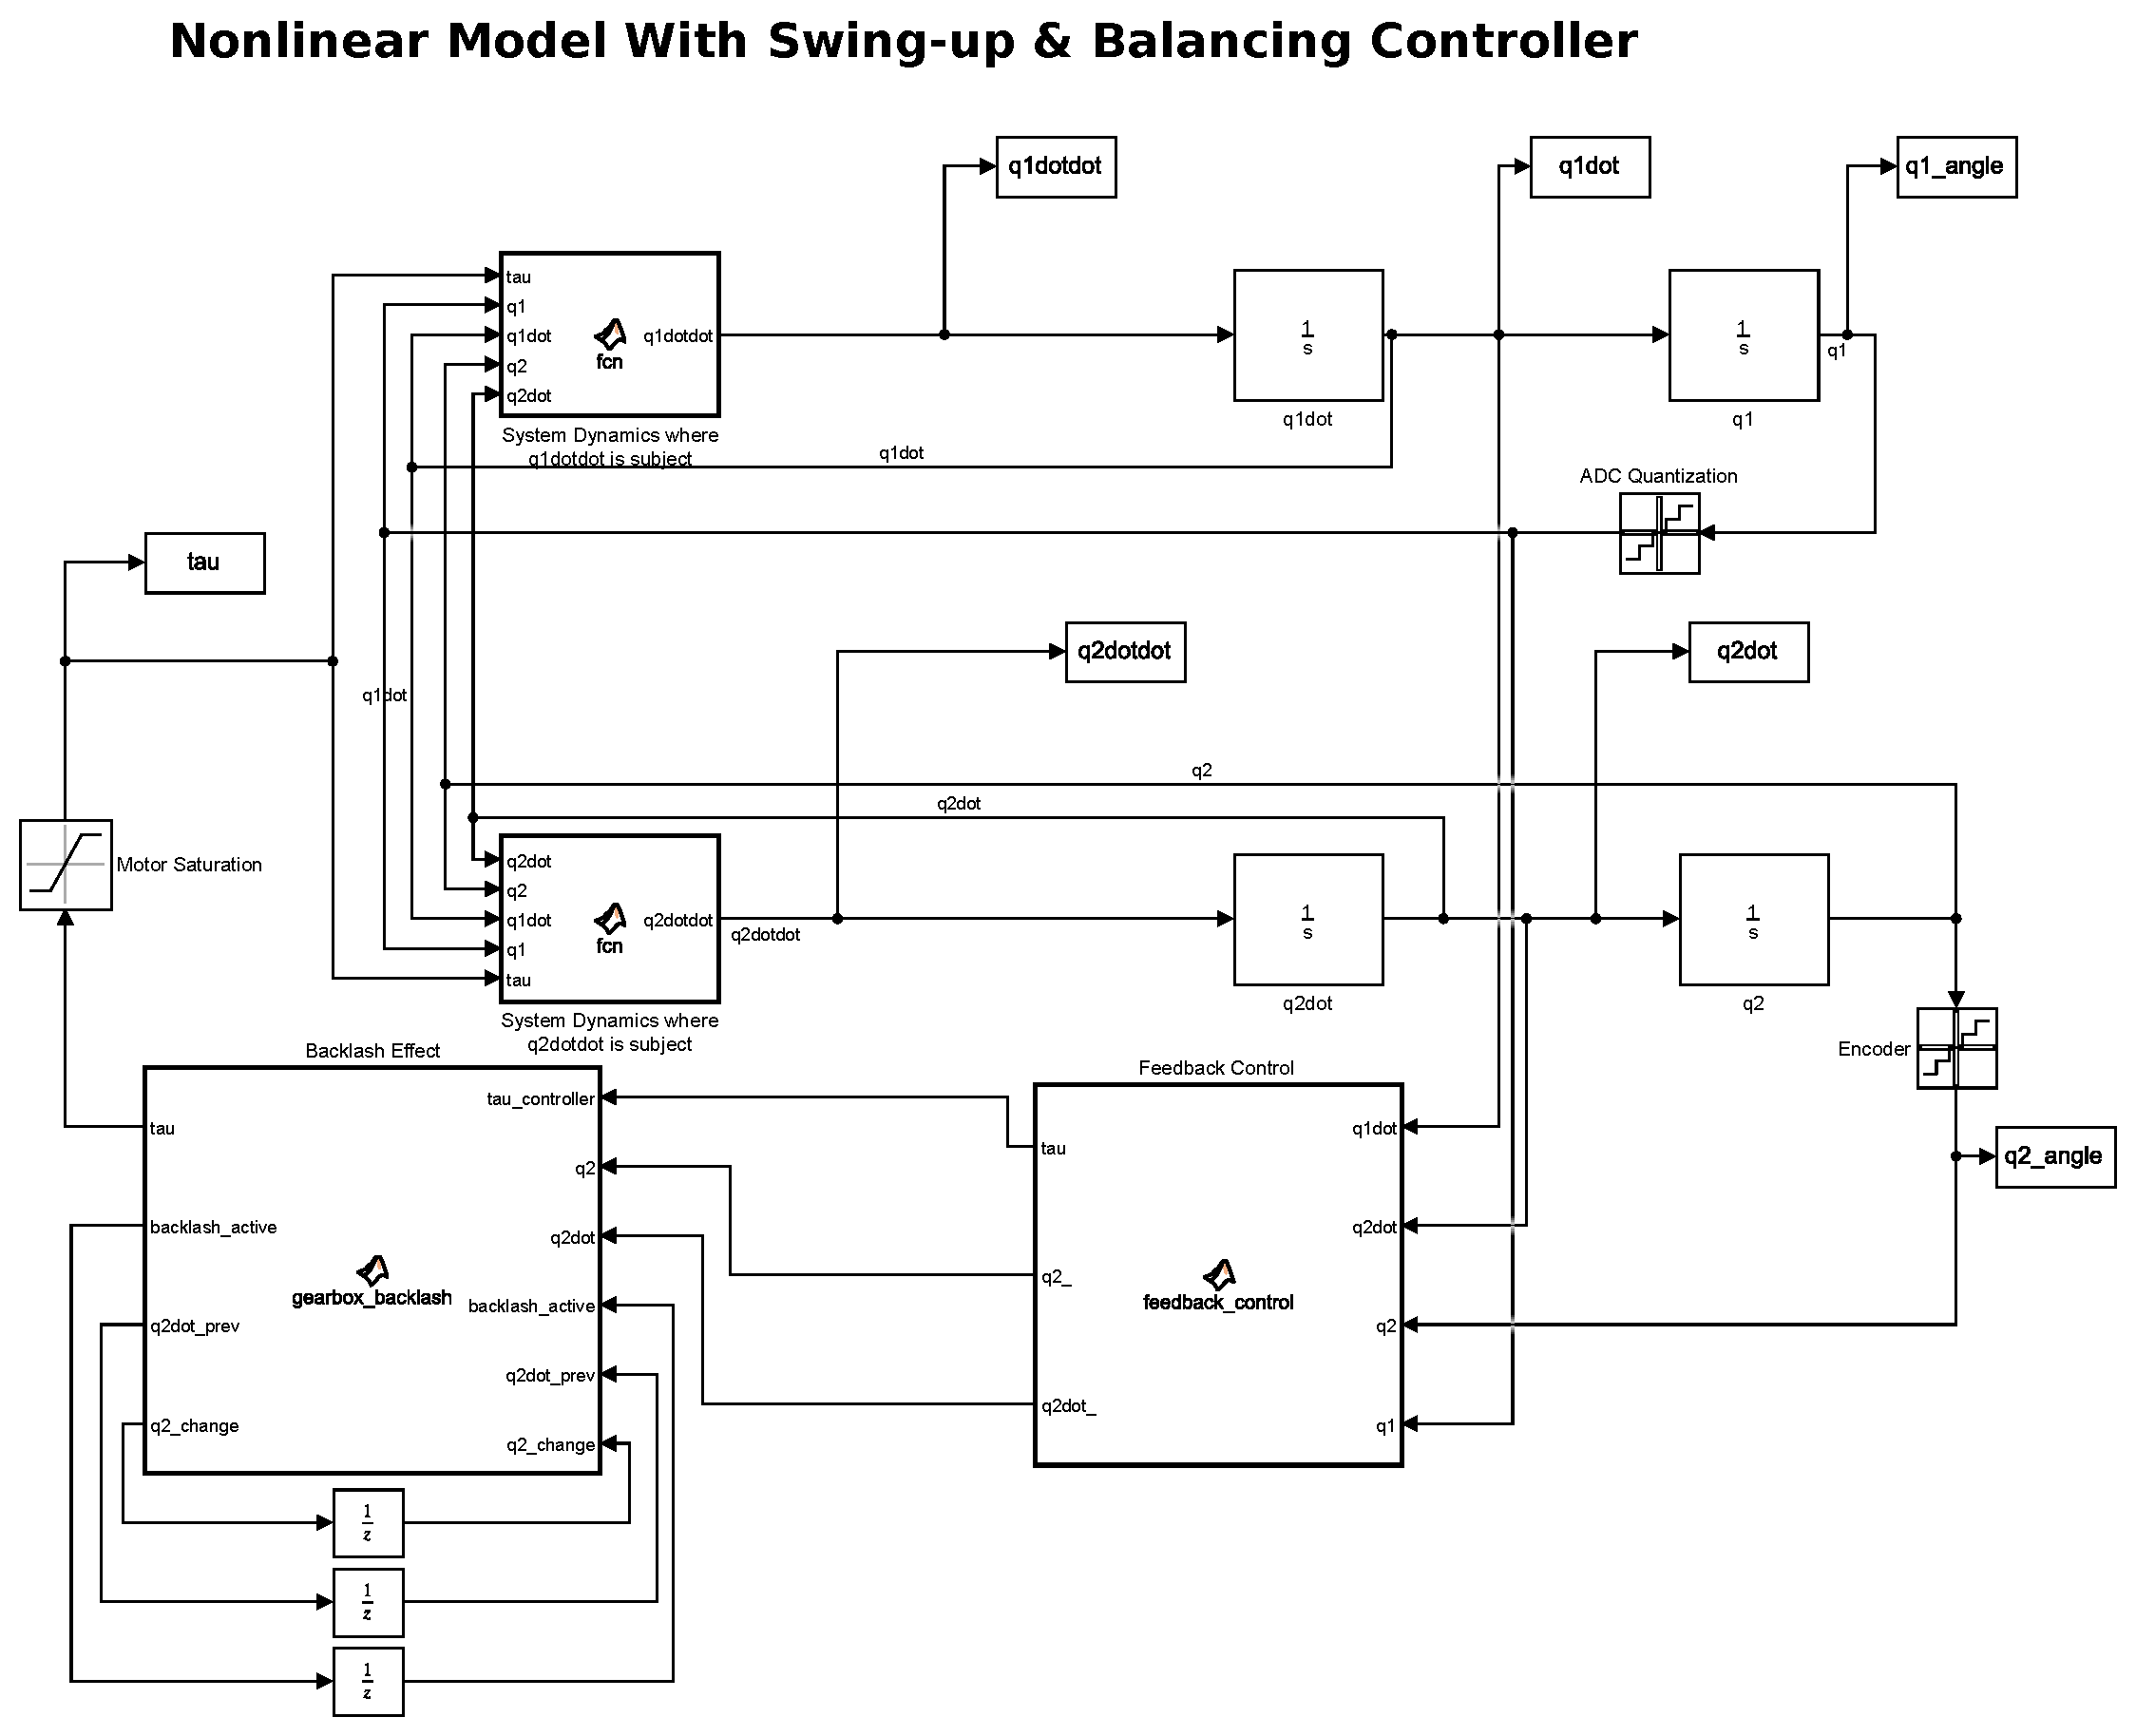
\includegraphics[scale=0.3]{./figs/simulink/latex_simulink.eps}
	\caption{MATLAB Simulink Model}
	\label{fig:sim_nonlinearfeedback}
\end{figure}

\section{System Identification}
\label{sec:system_identification}
%WHAT you are going to present in this chapter/section
%WHY you are presenting it, and
%HOW you are going to present it?

The system identification tests are done to determine the characteristics that describe the behaviour of the system. These characteristics include the damping ratio's and natural frequencies of the system. These characteristics will be presented by showing measured responses and how these responses can be modelled. \\

The project started off with a previous physical model which provided realistic system parameters to allow the simulation to be an acceptable representation of a physical model. From using these previous system parameters the simulation provided a set of specifications for the new mechanical design. All responses shown and values calculated are based on the new mechanical design parameters shown in Table \ref{table:system_param}.\\


		\begin{table}[]
	\centering
	\begin{tabular}{|c|c|}
		\hline
		System Parameter & Value \\
		\hline
		\hline
		$L_{1}$ & \SI{0.235}{m} \\
		\hline
		$L_{2}$ & \SI{0.310}{m} \\ 
		\hline
		$I_{A}$ & \SI{ 0.0022}{kg\cdot m^2}\\
		\hline
		$I_{B}$ & \SI{0.0043}{kg\cdot m^2}\\
		\hline
		$m_{1}$ & \SI{0.576}{kg}\\
		\hline
		$m_{2}$ & \SI{0.563}{kg} \\
		\hline
		$l_{1}$ & \SI{0.205}{m}\\
		\hline
		$l_{2}$ & \SI{0.194}{m}\\
		\hline
	\end{tabular}
	\caption{System Parameters}
	\label{table:system_param}
\end{table}


The system is described by two independent parameters and is expected to contain two natural frequencies each accompanied by a damping coefficient. The first natural frequency of the system was determined by inspecting the response of the system when starting at an initial condition and keeping $\phi = \SI{0}{\radian}$ throughout the response. This was done by using a lightweight PVC pipe that has negligible effect on the weight of the system. The actuated pendulum and unactuated pendulum are constrained to this pipe to ensure the two pendulums stay in-line with each other and thus ensuring $\phi = \SI{0}{\radian}$. The response of the system is shown in Figure \ref{fig:q1_response} starting at an initial condition of roughly $\theta = \SI{30}{\degree}$. The accuracy of the initial conditions is of little importance, but must allow the response to contain a few oscillations to accurately determine the parameter of interest.\\

\begin{figure}[h]
	\centering
	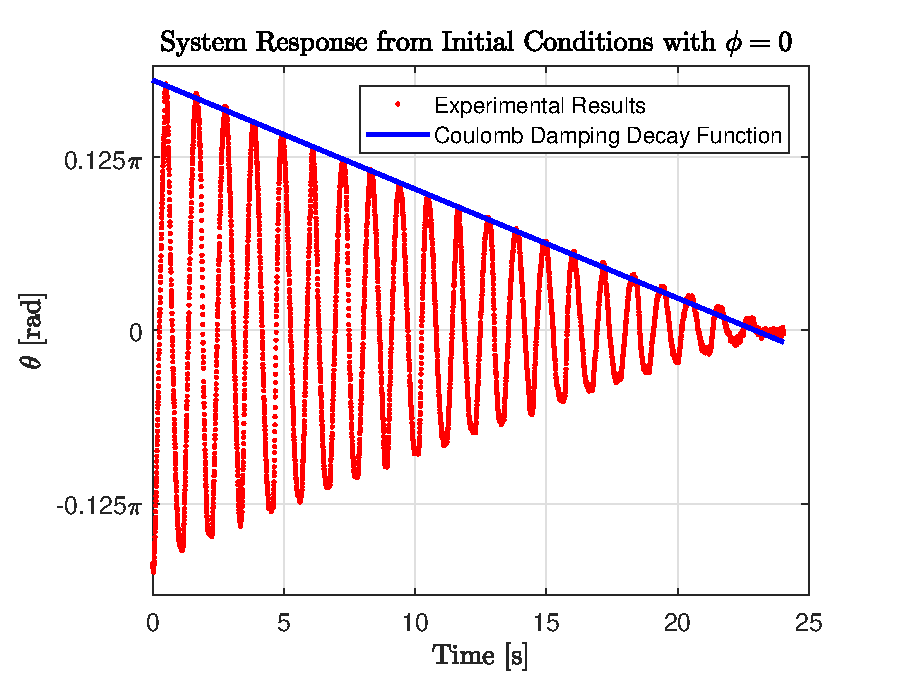
\includegraphics[scale=1]{./figs/q1_initial_response.eps}
	\caption{Initial Condition System Response while $ \phi = \SI{0}{rad} $ }
	\label{fig:q1_response}
\end{figure}


The second natural frequency was determined by analysing the response of the system when $\phi$ starts at an initial condition and keeping $\theta = \SI{0}{\radian}$ throughout the response. This was accomplished by constraining the unactuated pendulum using hard stops. Figure \ref{fig:q2_response} shows the measured response of the system when $\phi$ starts at an initial condition and keeping $\theta = \SI{0}{\radian} $.\\

\begin{figure}[h]
	\centering
	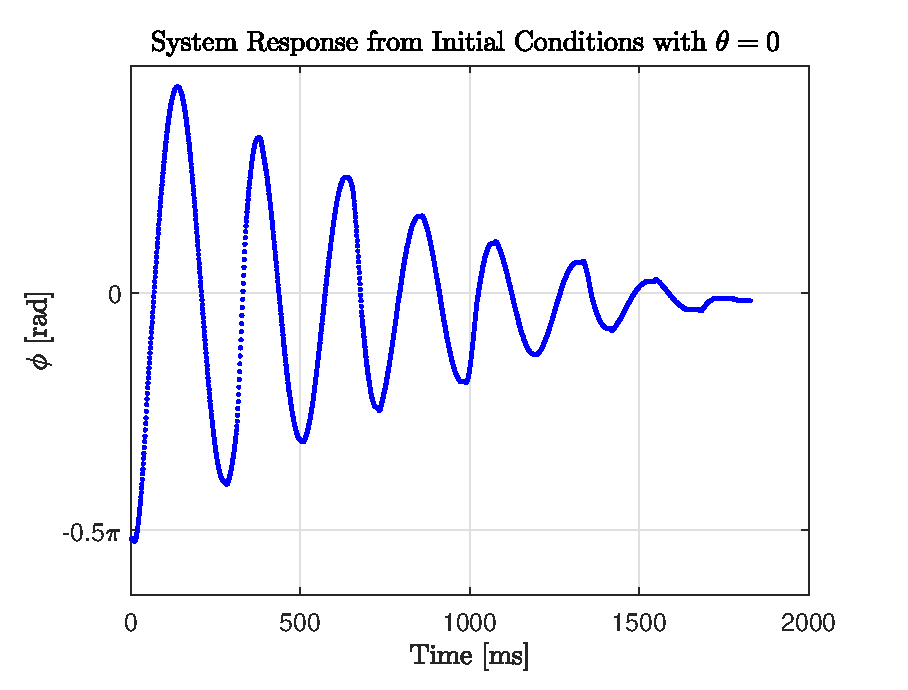
\includegraphics[scale=1]{./figs/q2_initial_response.eps}
	\caption{Initial Condition System Response while $ \theta = \SI{0}{rad} $ }
	\label{fig:q2_response}
\end{figure}

The responses shown in Figure \ref{fig:q1_response} and \ref{fig:q2_response} oscillate at the damped natural frequency $\omega_{d}$. The damped natural frequency was determined by measuring the time difference between peaks. The practical results contains a variation on the time difference between peaks and thus the mean of the time differences were calculated and shown in Table \ref{table:system_characteristic}.\\

The friction torques, $f_{c_{1}}$ and $f_{c_{2}}$ that were set as unknowns in the derivation of the robotic gymnast will be expanded on in the following section by analysing how the decaying of the responses can be characterised.\\

The response shown in Figure \ref{fig:q1_response} is under the influence of coulomb damping due to the response being characterised by the amplitude decaying linearly with a constant slope. Coulomb damping is caused by sliding friction and its torque is opposite to the direction of rotation \citep{coulomb_friction}. It is thus characterised as  $$ f_{c_{1}} = 
\left \{
\begin{tabular}{cc}
$ -\mu N $ & $ \dot{\theta}> 0 $\\
$ 0 $ & $ \dot{\theta} = 0$\\
$\mu N$ &   $ \dot{\theta} < 0$ \\
\end{tabular}
\right \}
$$

It is shown in \citet{coulomb_friction} that the slope is defined as 
\begin{equation} \label{eq:coulomb_slope}
-\frac{2\mu N \omega_{n}}{\pi mg}
\end{equation}

where $N$  is the normal force. The slope seen in the decay function in Figure \ref{fig:q1_response} was calculated using linear regression and by knowing the terms in equation (\ref{eq:coulomb_slope}) the combined $\mu N$ term can be calculated as shown in Table \ref{table:system_characteristic}.\\

The response shown in Figure \ref{fig:q2_response} is under the influence of viscous damping due to the amplitude decaying exponentially with time and this behaviour is modelled by the following equation: $$\tau(t) = Ae^{-\zeta \omega_{n}t}$$ where $\omega_{n}$ is the natural frequency, $\zeta$ the damping ratio of the system and $A$ represents the initial amplitude. The damped natural frequencies of the system have already been determined and linear regression was used to determine the best $\zeta$ that will fit the measured data. The decaying function is shown in Figure \ref{fig:q2_response} with the $\zeta$ value shown in Table \ref{table:system_characteristic}. It is visible from the response that the damping ratio fits the data well and only starts to deviate near steady state.\\

The damping moment, $f_{c_{2}}$ that develops between the stator and rotor of the hinge can then be characterised as $2\zeta\omega_{n}(\dot{\phi}-\dot{\theta})$. The subtraction of $\dot{\theta}$ is due to the rotor of the hinge rotating relative to the stator.

\begin{table}[]
	\centering
	\begin{tabular}{|c|c|}
		\hline
		System Characteristic & Mean\\
		\hline
		\hline
		$ \omega_{d_{1}} $ &$ \SI{3.4683}{rad/s}$ \\
		\hline
		$ \omega_{d_{2}} $ &$ \SI{3.88}{rad/s}$  \\ 
		\hline
		$ f_{c_{1}} $ &$ \SI{0.024}{Nm}$  \\
		\hline
		$ f_{c_{2}} $ &$ \SI{0.013}{\frac{Nm\cdot s}{rad}}$  \\ 
		\hline
		$ \zeta_{2} $ &$ \SI{0.0963}{}$\\
		\hline
	\end{tabular}
	\caption{Experimental System Characteristics}
	\label{table:system_characteristic}
\end{table}


\section{Model Validation}
%WHAT you are going to present in this chapter/section
%WHY you are presenting it, and
%HOW you are going to present it?
The model implemented in simulation must be able to describe the physical model to an acceptable degree to allow any further developments on the simulated model. The simulated model will be validated by comparing the experimental system characteristic values to those attained in simulation.\\

Table \ref{table:experiment_vs_simulation} shows the experimental values determined in the previous section against the simulation characteristic and indicates the simulation model represents the physical model well.\\

Figure \ref{fig:sim_vs_measured_q1} and \ref{fig:sim_vs_measured_q2} provides a visual verification of which the damping effects are modelled to an acceptable degree. It is visible that the simulated response fits the experimental response well, matching the frequency of oscillation during high velocities and large angles. It is only near steady state where the simulated responses deviates a little. \\

Figure \ref{fig:sim_vs_measured_q2} does not describe the damping effect throughout the entire response. This is expected due to the damping force not being constant throughout the response as seen in Figure \ref{fig:q2_response}. The average of the damping coefficients were selected and results in variances.


\begin{table}[]
	\centering
	\begin{tabular}{|c|c|c|}
		\hline
		System & $\omega_{d_{1}}$  & $\omega_{d_{2}}$ \\
		\hline
		\hline
		Experimental  & 3.96 &  3.88\\
		\hline
		Simulation & 6.75 & 6.704\\ 
		\hline
	\end{tabular}
	\caption{Experimental Characteristics vs Simulation Model Characteristic}
	\label{table:experiment_vs_simulation}
\end{table}

\begin{figure}[h]
	\centering
	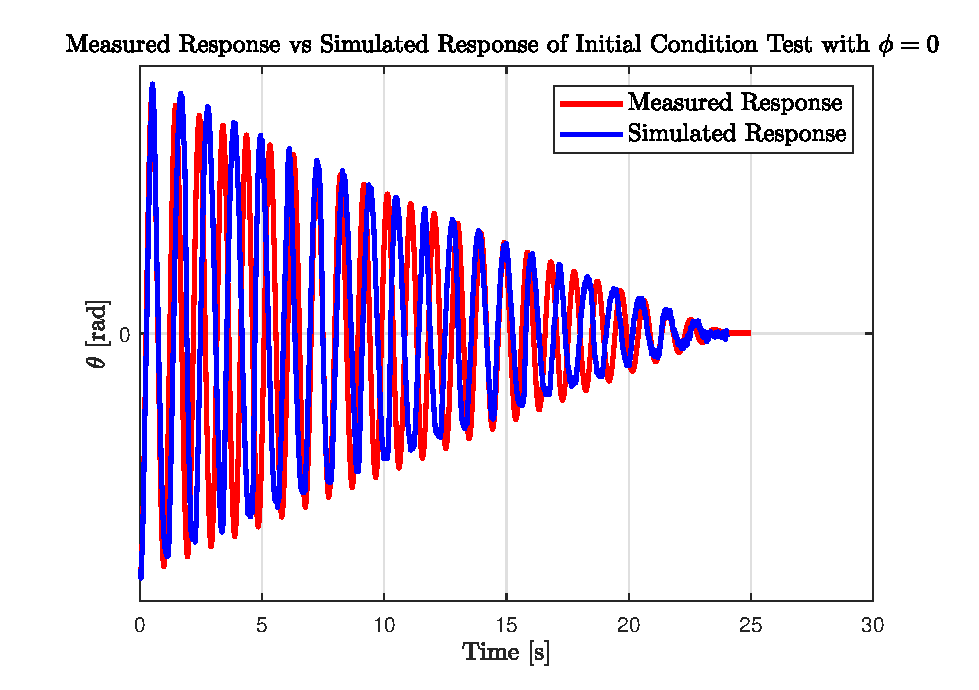
\includegraphics[scale=0.8]{./figs/sim_vs_measured_q1.eps}
	\caption{Comparison between Simulated and Measured Response with $\phi = \SI{0}{\radian}$ throughout}
	\label{fig:sim_vs_measured_q1}
\end{figure}

\begin{figure}[h]
	\centering
	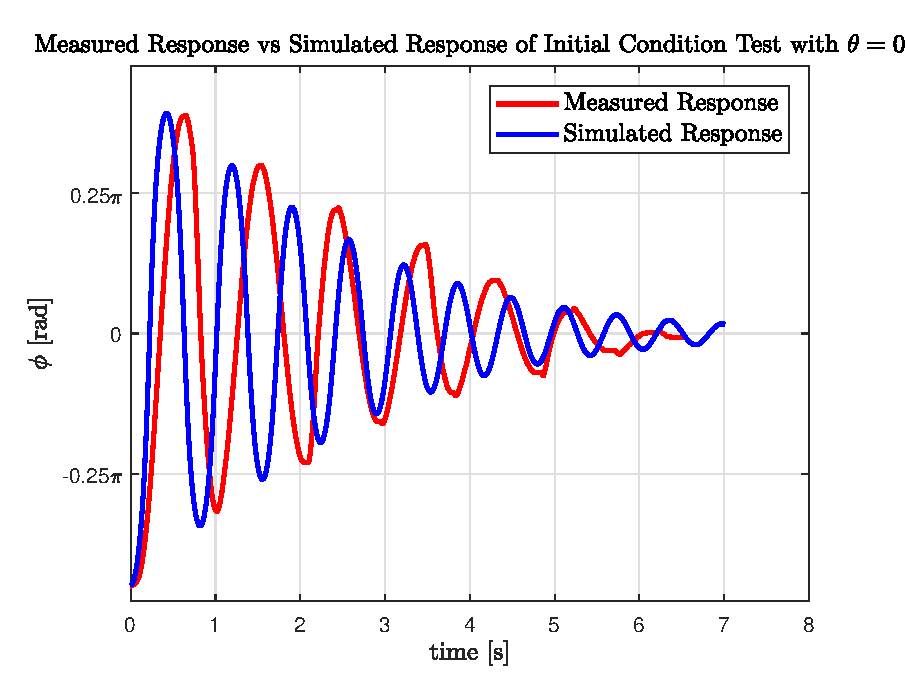
\includegraphics[scale=0.8]{./figs/sim_vs_measured_q2.eps}
	\caption{Comparison between Simulated and Measured Response with $\theta = \SI{0}{\radian}$ throughout}
	\label{fig:sim_vs_measured_q2}
\end{figure}



\chapter{Feedback Control Design}
\label{chp:controller}
This chapter presents the design of the feedback control laws to swing up and balance the robotic gymnast. Two separate controllers are used, one to swing up the robotic gymnast from the hanging position to the vertical position, and another to catch and balance the robotic gymnast when it reaches the inverted position. The design of the balancing controller will be presented first, followed by the design of the swing up controller. The chapter will conclude with a simulation that illustrates the integrated swing up and balancing of the system, starting with the swing up controller and switching over to the balancing controller.

\section{Balancing Controller}
% WHAT you are going to present in this chapter/section
% WHY you are presenting it, and
% HOW you are going to present it

Provided the robotic gymnast is in the vicinity of the unstable equilibrium position, a balancing controller is required to balance the system in the inverted position. The design approach was based on the premise that the swing-up controller will swing the robotic gymnast to the vicinity of the unstable equilibrium position where the balancing controller will take over. This section will focus on the aspects required to implement this balancing controller.\\


\subsection{Controller Architecture}
\begin{figure}
	\centering
	% System Combination
% Harish K Krishnamurthy <www.ece.neu.edu/~hkashyap/>
\documentclass{article}

\usepackage{tikz}
\usetikzlibrary{shapes,arrows,shadows}
\usepackage{amsmath,bm,times}
\newcommand{\mx}[1]{\mathbf{\bm{#1}}} % Matrix command
\newcommand{\vc}[1]{\mathbf{\bm{#1}}} % Vector command

\begin{document}
	% Define the layers to draw the diagram
	\pgfdeclarelayer{background}
	\pgfdeclarelayer{foreground}
	\pgfsetlayers{background,main,foreground}
	
	% Define block styles used later
	
	\tikzstyle{sensor}=[draw, fill=blue!20, text width=5em, 
	text centered, minimum height=2.5em,drop shadow]
	\tikzstyle{ann} = [above, text width=5em, text centered]
	\tikzstyle{wa} = [sensor, text width=10em, fill=red!20, 
	minimum height=6em, rounded corners, drop shadow]
	\tikzstyle{sc} = [sensor, text width=13em, fill=red!20, 
	minimum height=10em, rounded corners, drop shadow]
	
	% Define distances for bordering
	\def\blockdist{2.3}
	\def\edgedist{2.5}
	
	\begin{tikzpicture}
	\node (wa) [sensor]  {$\boldsymbol{\dot{x}}= \boldsymbol{A}\boldsymbol{x}+\boldsymbol{B}$};
	\path (wa.south)+(0,-1) node (feedback) [sensor] {$u = -\boldsymbol{K}\boldsymbol{x}$};
	
	\path (wa.east)+(\blockdist/1.5,0) node (C) [sensor] {$\boldsymbol{C}$};
	\path (C.east)+(\blockdist/1.5,0) node (Y) [sensor] {$\boldsymbol{y}$};
	
	
	\path [draw, ->,thick] (wa.east) -- node [above] {} 
	(C.west);
	
	\path [draw, ->,thick] (C.south) |- node [above] {} 
	(feedback.east);
	
	\path [draw, ->,thick] (C.east) -- (Y.west);
	
	\path [draw, ->,thick] (feedback.west) -| ([xshift=-1cm]wa.west) -- (wa.west) {};
	
	%\path [draw, ->,] (C.east) -- node [above] {} 
	%	(Y.west);
	
	%\path (wa.south) +(0,-\blockdist) node (asrs) {System Combination - Training};
	
	%\begin{pgfonlayer}{background}
	%   \path (asr1.west |- asr1.north)+(-0.5,0.3) node (a) {};
	%  \path (wa.south -| wa.east)+(+0.5,-0.3) node (b) {};
	% \path (C.east |- asrs.east)+(+0.5,-0.5) node (c) {};
	
	%\path[fill=yellow!20,rounded corners, draw=black!50, dashed]
	%   (a) rectangle (c);           
	% \path (asr1.north west)+(-0.2,0.2) node (a) {};
	
	%\end{pgfonlayer}
	
	\end{tikzpicture}
	
\end{document}}
	\caption{State Space Representation of the Balancing Controller}
	\label{fig:linearSys2}
\end{figure}

Figure \ref{fig:linearSys2} shows the block diagram that implements the balancing controller, and it is clear that the state space representation of the system was used. This requires the system to be a linear time invariant (LTI) system, but the system described in equation (\ref{eq:condense1}) and (\ref{eq:condense2}) are not linear. This requirement was satisfied by linearising the system.\\

Another aspect of the balancing controller is that there are no reference input to instruct the controller to guide the robotic gymnast to the unstable equilibrium position. The linearised system at the inverted position is unstable. The feedback control makes the close loop system stable around the inverted state that would normally be unstable for the uncontrolled system.


\subsection{Requirements/Specifications and Constraints}
The independent parameters, $\phi$ and $\theta$, will be condensed from now on as a vector describes as $$ \vec{q} = 
\begin{bmatrix}
\theta \\
\phi
\end{bmatrix}
$$


The requirements set out for the balancing controller were to bring the robotic gymnast to the unstable equilibrium position from an initial condition range of:
$$ \vec{q_{i}} \in 
\left \{
\begin{tabular}{c}
$ [\SI{177}{\degree}, \SI{183}{\degree}]   $\\
$ [\SI{-5}{\degree} , \SI{5}{\degree}] $ \\

\end{tabular}
\right \}
$$


The response must have a settling time of 1 seconds and a percentage overshoot $M_{p}$ of 10\%.\\

These requirements were selected to give the swing-up controller enough margin to bring the system to the vicinity of the unstable equilibrium position where the balancing controller is capable of balancing.\\


\subsection{Plant Linearisation}

As mentioned previously, to implement the state space representation the system must be a LTI system. This was achieved by using the Taylor Series Expansion to linearise the system at the unstable equilibrium position.\\

The system is linearised at 
$$ [\vec{q_{s}},\dot{\vec{q_{s}}},\ddot{\vec{q_{s}}}]^{T}=[\pi,0,0,0,0,0]$$
with the mathematical details shown in Appendix \ref{sec:linerisation}. This linearised model can then be written in the state space form to implement a feedback gain. The state space variables are chosen as $\Delta{\vec{q}}$ and $\Delta{\dot{\vec{q}}}$ which results in the state space representation as:  $$ \dot{\vec{q}} = \boldsymbol{A}\Delta{\vec{q}} + \boldsymbol{B}u $$ $$ \vec{y} = \boldsymbol{D}\Delta{\vec{q}} + \boldsymbol{0}u $$

The poles of the system are identified by determining the eigenvalues of the $\boldsymbol{A}$ matrix. The linearised system remains a coupled system which results that the quadratic eigenvalue problem shown in equation (\ref{eq:quadratic_eigen}) was required to be solved to identify the poles. The solved quadratic eigenvalue problem results in the following eigenvalues using the system parameters in Table \ref{table:system_param}.

\begin{equation} \label{eq:quadratic_eigen}
Q(\lambda) =\lambda^{2}M + \lambda C + K
\end{equation}

$$
\vec{s} = 
\begin{bmatrix}
-12.06 \\
-5.05 \\
10.64 \\
5.01 \\
\end{bmatrix}
$$

The eigenvalues of the system are all real indicating the response of the system when disturbed is an exponential function. This can be explained by realising the linearised system is modelled as a single pendulum. Once the single pendulum is disturbed from the unstable equilibrium position it would continue to rotate downwards and not with an oscillatory response.\\

The identified coulomb damping that the unactuated pendulum experience shown in Figure \ref{fig:q1_response} is not possible to linearised. This friction was approximated as viscous damping in the linear model and was acceptable due to the physical model showing characteristic of viscous damping near steady state visible in Figure \ref{fig:q1_response}.


\subsection{Full State Feedback Design}
The poles of the system are pairs of positive and negative real poles that indicate an unstable system. This is expected due to the system being linearised at the unstable equilibrium position. When the linearised system is at rest, any disturbance will result in a theoretically infinite growth of the state variables, but this behaviour can be controlled by introducing feedback. \\

These poles will be moved to the desired position by using the method of dominant poles. The method of dominate poles chooses a pair of the poles for the closed-loop system and select the other open-loop poles to have real parts with much larger natural frequencies. This allows the higher-order system response to be characterised as a second-order response \citep{textbook}. \\

Assuming a second order system and using the requirements defined, the pole locations can be calculated using equation (\ref{eq:overshoot}) and (\ref{eq:settling_time})
\begin{equation} \label{eq:overshoot}
M_{p} = \exp(\frac{-\pi \zeta}{ \sqrt{1-\zeta^2}})
\end{equation}

\begin{equation} \label{eq:settling_time}
t_{s} = \frac{4.6}{\zeta \omega_{n}}
\end{equation}

and knowing the poles are described seen in equation (\ref{eq:poles}) 

\begin{equation} \label{eq:poles}
p = \zeta \omega_{n} \pm j\omega_{d}
\end{equation}

results in the desired pole locations as:
 $$
 \vec{p} = 
 \begin{bmatrix}
  -4.6 + j6.13 \\
-4.6 - j6.13 \\
-23\\
-23\\
 \end{bmatrix}
 $$


\subsection{Simulation Response}
\begin{figure}[h]
	\centering
	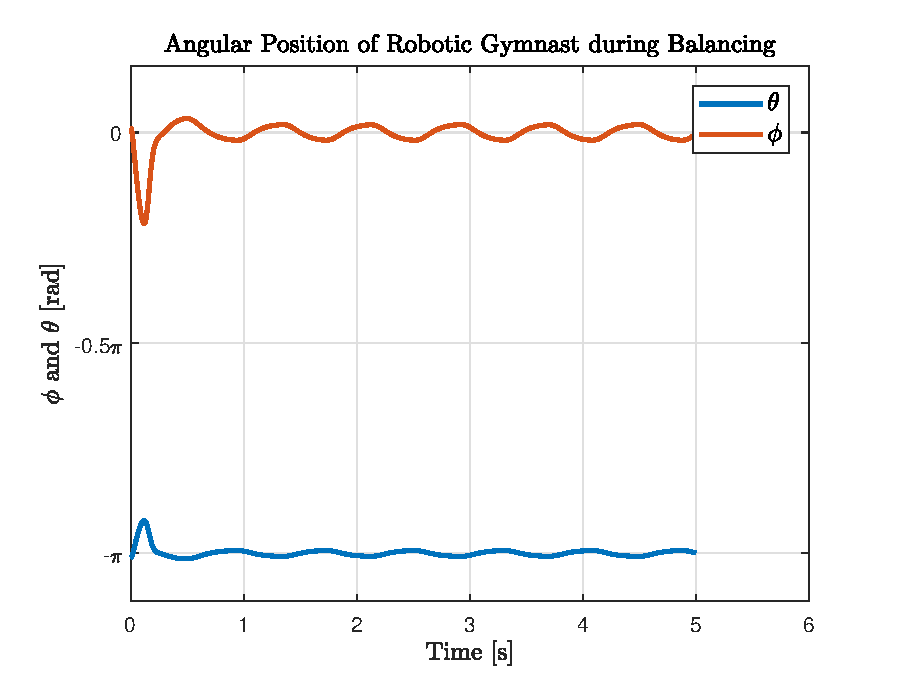
\includegraphics[scale=1]{./figs/balancing}
	\caption{Balancing of the Robotic Gymnast}
	\label{fig:balance}
\end{figure}



Figure \ref{fig:balance} shows the robotic gymnast balancing around the unstable equilibrium position from an initial condition of $$ \vec{q_{i}} = 
\begin{bmatrix}
$\SI{183.6}{\degree}$\\
$\SI{-9}{\degree}$ \\
\end{bmatrix}
$$ 

The response shows that the controller meets the requirement of balancing the robotic gymnast from required initial condition and reaches steady state within 1 seconds. The overshoot requirement of 10\% has also been achieved on the unactuated pendulum.\\

\section{Swingup Controller}
% WHAT you are going to present in this chapter/section
% WHY you are presenting it, and
% HOW you are going to present it
For the robotic gymnast to swing from the stable equilibrium position to the unstable equilibrium position the feedback control must deal with the nonlinearities of the system.The design approach, including how the feedback controller handles the nonlinearities, is explained in the following section.

\subsection{Controller Architecture}
\begin{figure}[h]
	\centering
	\documentclass{article}

\usepackage{tikz}
\usetikzlibrary{shapes,arrows}
\usepackage{amsmath,bm,times}
\newcommand{\mx}[1]{\mathbf{\bm{#1}}} % Matrix command
\newcommand{\vc}[1]{\mathbf{\bm{#1}}} % Vector command

\begin{document}
	\pagestyle{empty}
	
	% We need layers to draw the block diagram
	\pgfdeclarelayer{background}
	\pgfdeclarelayer{foreground}
	\pgfsetlayers{background,main,foreground}
	
	% Define a few styles and constants
	\tikzstyle{sensor}=[draw, fill=blue!20, text width=5em, 
	text centered, minimum height=2em]
	\tikzstyle{ann} = [above, text width=5em]
	\tikzstyle{block} = [sensor, text width=6em, fill=red!20, 
	minimum height=4em, rounded corners]
	\tikzstyle{sum}=[draw, fill=red!20, circle, node distance = 2cm]
	
	\tikzstyle{longblock} = [sensor, text width=10em, fill=red!20, 
	minimum height=4em, rounded corners,minimum width=6em]
	
	\def\blockdist{2.5}
	\def\edgedist{2.5}
	
	
	
	\noindent\makebox[\textwidth]{
	\begin{tikzpicture}[scale=0.8]
	% plant block
	\node (plant) [block] {Non-Linear Plant};
	
	% collocated blovk
	\path (plant)+(0,-\blockdist) node (collinear) [block] {Collocated\ Linearisation};
	
	% Annotation
%	\path (plant)+(1.5*\blockdist,0) node (output) [ann] { [ $\ddot{\theta}$ \\ $\dot{\phi}$ ] };
	
	\path (plant)+(1.2*\blockdist,0) node (output) [ann] { 
$\begin{bmatrix}
$$\ddot{\theta}$$ \\ $$\ddot{\phi}$$ 
\end{bmatrix}$
};
	
	%sumation block 1
	\path (plant)+(-\blockdist,0) node (suma1) [sum]{\Large$\Sigma$};
	
	% Non-linear control law
	\path (plant)+(-2.2*\blockdist,0) node (nonlinear) [longblock]{Non-Linear Law \ $v = K_{p}(\phi^{d}-\phi)-K_{d}\dot{\phi}$};
	
	%sumation block 2
	\path (nonlinear)+(-1.2*\blockdist,0) node (suma2) [sum]{\Large$\Sigma$};

	% Desired input
	\path (suma2)+(-1.2*\blockdist,0) node (desired) [longblock]{Desired Trajectory \ $\phi^{d} = \alpha \tan(\dot{\theta})$};

%%%%%%%%%%%%%%%%%%%%%%%%%%%%%%%%%%%%%%%%%%%%%%%%%%%%%%%%%%%%%%%%%%%%%%%%%%%%%%%%%%%%%%%%%%%%%%%%%%%%%%%%%%%%%%%%%%%%%%%%%%
	% plant to output	
%	\draw [->,thick] (plant) -- node [anchor=north east] {} + (\edgedist,0) 
%	node[right] {$[\theta$ $\phi$ $\dot{\theta}$ $\dot{\phi}$ $\ddot{\phi}$  $\ddot{\theta}]$};
	
	%plant to output
	\draw [->,thick] (plant.east) -- ([xshift=1cm]plant.east) {};
	% plant to collocated
	\draw[->,thick] ([xshift=0.5cm]plant.east) -- ([xshift=0.5cm]collinear.east) -- (collinear.east) {};
	
	% collocated lineariation to Sigma
	\draw[->,thick] (collinear.west) -| (suma1.south) {};
	
	%sigma to non-linear plant
	\draw[->,thick] (suma1.east) -- (plant.west) {};
	
	% non-linear law to sigma
	\draw[->,thick] (nonlinear.east) -- (suma1.west) {};
	
	% sigma2 to non linear
	\draw[->,thick] (suma2.east) -- (nonlinear.west) {};

	% Desired input to sigma
	\draw[->,thick] (desired.east) -- (suma2.west) {};
	
	% collocated to sigm2
	\draw[->,thick] (collinear.west) -| (suma2.south) {};
	






	% Now it's time to draw the colored IMU and INS rectangles.
	% To draw them behind the blocks we use pgf layers. This way we  
	% can use the above block coordinates to place the backgrounds   
	\begin{pgfonlayer}{background}
	% Compute a few helper coordinates
%	\path (gyros.west |- naveq.north)+(-0.5,0.3) node (a) {};
%	\path (INS.south -| naveq.east)+(+0.3,-0.2) node (b) {};
	%\path[fill=yellow!20,rounded corners, draw=black!50, dashed]
	%(a) rectangle (b);
%	\path (gyros.north west)+(-0.2,0.2) node (a) {};
	%\path (IMU.south -| gyros.east)+(+0.2,-0.2) node (b) {};
%	\path[fill=blue!10,rounded corners, draw=black!50, dashed]
%	(a) rectangle (b);
	\end{pgfonlayer}

\end{tikzpicture}
}
	
\end{document}
	\caption{Block Diagram of the Non-Linear Controller}
	\label{fig:nonlinear_controller_arch}
\end{figure}
Figure \ref{fig:nonlinear_controller_arch} shows a high-level block diagram of the multiple parts of the swing-up controller. These parts are required to work in unison to allow the robotic gymnast to swing.\\


The collocated linearisation block linearises the response from the motor torque input to the actuated pendulum angle output. The linear control law controls the angle of the actuated pendulum $\phi$ to follow a command reference angle ${\phi}^d$. The controller gains $Kp$ and $Kd$ are designed to provide a good transient response. The swing up trajectory generator implements a nonlinear control law that provides reference commands $\phi^3$ for the actuated pendulum angle $\phi$, as a function of the angular rate $\dot{\theta}$ of the unactuated pendulum. The maximum angle command for the actuated pendulum is limited by the $\arctan$ function and the constant parameter $\alpha$.\\\

The swing-up controller implements classical control theory approach where gains are selected to characterise the response of the system based on the error of the desired trajectory and the actual trajectory of the system.\\

Each of the blocks shown in the block diagram will be discussed in the section below.


\subsection{Requirements/Specifications and Constraints}
% WHAT you are going to present in this chapter/section
% WHY you are presenting it, and
% HOW you are going to present it
The requirements of the swing-up controller is to swing the robotic gymnast upwards under 30 seconds in the vicinity of the unstable equilibrium position. The vicinity of the unstable equilibrium position is defined as $\theta = \SI{2\pi}{\radian} \pm \frac{\pi}{30}$ and $\phi \in [-5^{\circ},5^{\circ}]$.\\

The constraint placed on the swing up controller is that its torque command to the motor actuator should not exceed 50\% of the stall torque of the motor.

The first requirement is to provide a feasible solution to the swing-up of the robotic gymnast and allow the swing-up sequence to be captivating. The second requirement is to ensure the linear approximation of the system is acceptable when the balancing controller is active to bring the system to the inverted position and balance. The constraint placed was to increase the safety in testing and prolonging the life of the motor.\\

\subsection{Feedback Linearisation}
\citet{murray} showed that it is not possible to linearise the dynamics of the robotic gymnast using static state feedback and non-linear transformation, but that it is possible to achieve a linear response from one of the outputs of the system (either the actuated or the unactuated pendulum angle) using nonlinear feedback that provides partial feedback linearisation.\\

Collocated linearisation is a form of partial feedback linearisation where a non-linear control input $\tau$ is used to linearise the response of the actuated pendulum $\ddot{\phi}$. By analysing equation (\ref{eq:condense2}), the input $\tau$ was chosen to cancel all the non-linearities of the system and add an additional outer loop control input $v_{2}$ as seen in equation (\ref{eq:collocated_lin3}). This results in the unactuated pendulum to see a indirect force and the problem can be reduced to finding the outer loop control input to force the actuated pendulum to swing upwards \citep{spong_swingup}.

 The complete derivation is done by \citeauthor{spong_swingup} and the final result of the collocated linearisation is shown below.
\begin{equation} \label{eq:collocated_lin3}
\tau = d_{21}\ddot{\theta} + v_{2}d_{22}\ddot{\phi} + h_{2} + \psi_{2}
\end{equation}
\begin{equation} \label{eq:collocated_lin1}
d_{11}\ddot{\theta} + h_{1} + \psi_{1} = -d_{12}v_{2} \approx F
\end{equation}
\begin{equation} \label{eq:collocated_lin2}
\ddot{\phi} = v_{2}
\end{equation}

The subtle practical implication of using collocated linearisation is that the system being controlled must be well defined. If this is not the case the non-linear input $\tau$ will introduce other unwanted dynamics that could lead to undesirable behaviour.

\subsection{Nonlinear Control Law}

The ability to control the actuated pendulum to follow a desired trajectory, provides the possibility to increase the energy of the system if the correct trajectory is chosen. The increase of energy in the system will cause the pendulums to rise from their stable equilibrium position and start swinging upwards. The desired trajectory for ${\phi}$ was chosen as equation (\ref{eq:desired_phi}) determined by \citet{spong_swingup}.
\begin{equation} \label{eq:desired_phi}
\phi^{d} =  \alpha \arctan(\dot{\theta})
\end{equation}

This desired trajectory was derived by analysing a single pendulum and approximating the force it experiences as seen in equation (\ref{eq:collocated_lin1}). By using this approximation \citeauthor{spong_swingup} showed that the desired trajectory will increase the energy in the system. The desired trajectory also tries to allow the actuated pendulum to swing in phase with the non-actuated pendulum and by this approach the energy of the actuated pendulum is transferred to the unactuated pendulum \citep{spong_swingup}.\\

The outer loop control input, $v_{2}$, then implements the classical control approach where gains are selected to characterise the response of the system based on the error seen in equation (\ref{eq:v2}). 

   
\begin{equation} \label{eq:v2}
v_{2} = K_{p}(\phi^{d}-\phi)-K_{d}\dot{\phi}
\end{equation}

The coefficient $\alpha$ used in equation (\ref{eq:desired_phi}) constrains the actuated pendulum to stay within a interval of $ \phi \in [-\beta,\beta]$ where $\alpha < \beta$ \cite{spong_swingup}. This provides better control over the system to stay within the null controllability region when the system reaches the unstable equilibrium position.\\

Another side-effect of using the non-linear controller is that at rest the system will not start to swing-up. At rest, the conditions are: $\phi = \SI{0}{\radian}$ and $\dot{\phi} = \SI{0}{\radian/s}$, and results in the control output seen in equation (\ref{eq:v2}) to be zero. This effect was overcome by giving the system a small initial condition to start the swing-up controller.


\subsection{Simulation Response}
\begin{figure}[h]
	\centering
	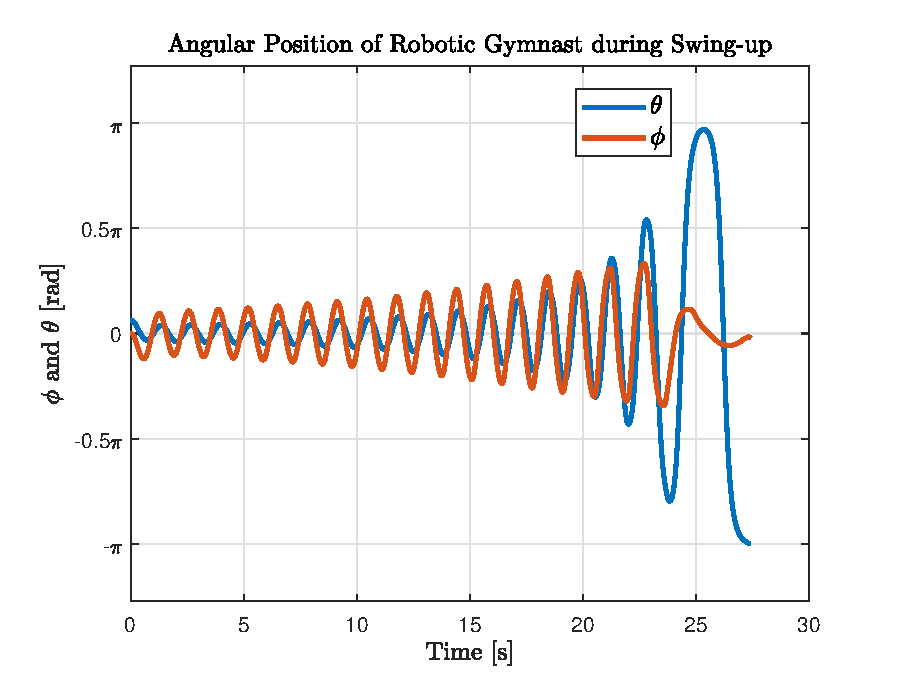
\includegraphics[scale=1]{./figs/swingup}
	\caption{Swing-up of the Robotic Gymnast}
	\label{fig:swingup}
\end{figure}

Figure \ref{fig:swingup} shows the swing-up controller swinging the robotic gymnast from the stable equilibrium position to the vicinity of the unstable equilibrium position with gain constants used shown in Table \ref{table:gain_constants}. There are a few interesting occurences in the responses mentioned in the previous section which needs to be brought to the attention of the reader.\\

\begin{table}[]
	\centering
	\begin{tabular}{|c|c|}
		\hline
		Gain Constant & Value \\
		\hline
		\hline
		$K_{p}$  & 58 \\
		\hline
		$K_{d}$  & 14 \\
		\hline
	\end{tabular}
	\caption{Gain Constant used during Simulation}
	\label{table:gain_constants}
	\end{table}

Firstly the robotic gymnast is required to start at an initial condition for the swing-up control law to be active and this is seen with $\theta$ starting at 11\textdegree. Secondly, the amplitude of $\phi$ is seen to decrease suddenly when the system nears the inverted position. This is due to $\alpha$ being reduced when the robotic gymnast nears the inverted position.\\

The response shows the swing-up controller meets the designed requirements by swinging the robotic gymnast to the vicinity of the unstable equilibrium within 30 seconds and $\theta$ and $\phi$ are in the designed region for the balancing controller to bring the system to the inverted position.



\section{Simulation Results}
\begin{figure}[h]
	\centering
	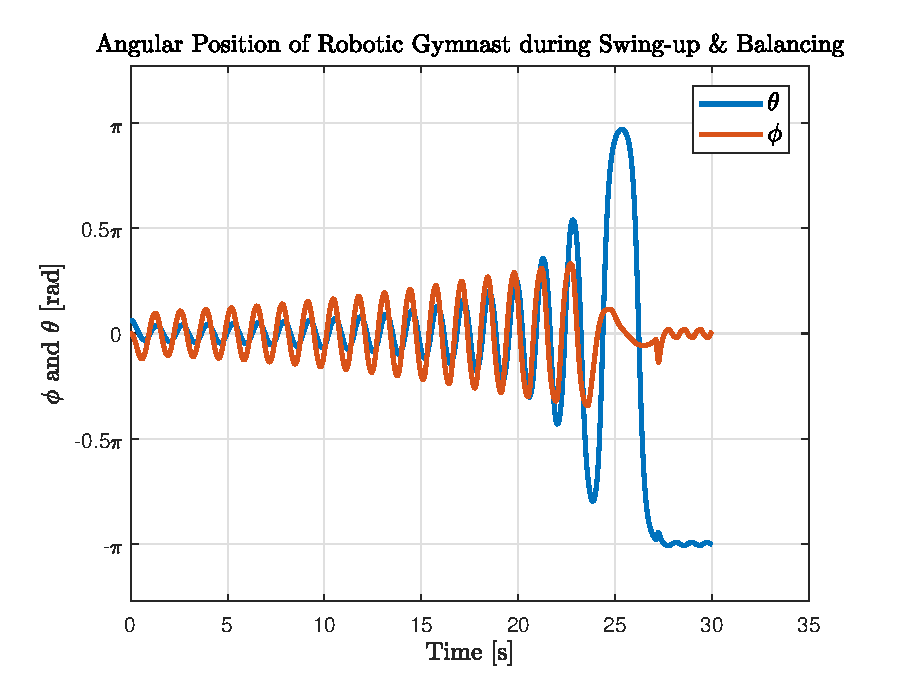
\includegraphics[scale=0.9]{./figs/swingup_balance}
	\caption{The Swing-Up \& Balancing of the Robotic Gymnast}
	\label{fig:swingup_balance}
\end{figure}

Once both controllers were capable of meeting the requirements set out, they needed to be combined to achieve the swing-up and balancing of the robotic gymnast. Figure \ref{fig:swingup_balance} shows the response of both controllers combined that achieved the swing-up and balancing.\\

During the swing-up the $\alpha$ value was reduced by the algorithm as it pass through the positions seen in equation (\ref{eq:alpha}).

\begin{equation}
\label{eq:alpha}
\alpha = 
\left \{
\begin{tabular}{cc}
$ \SI{90}{\degree}$\: & $  \theta < \SI{45}{\degree} 	$\\
$ \SI{45}{\degree}$\: & $  \SI{126}{\degree} < \theta > \SI{45}{\degree} $\\
$ \SI{12}{\degree}$\: & $ \SI{177}{\degree} < \theta > \SI{126}{\degree}$ \\
\end{tabular}
\right \}
\end{equation}

\chapter{Hardware Design and Implementation}
This chapter presents the design and implementation of the physical gymnastic robot that was used to determine the system characteristics. The design and implementation of the mechanical hardware is presented first, followed by the design of the electronic hardware. The chapter concludes with the tests that were performed to verify that the electronic hardware interfaces correctly with the motor driver.

\section{Mechanical Hardware}
\label{sec:mechanical_hardware}

\begin{figure}[h]
	\centering
	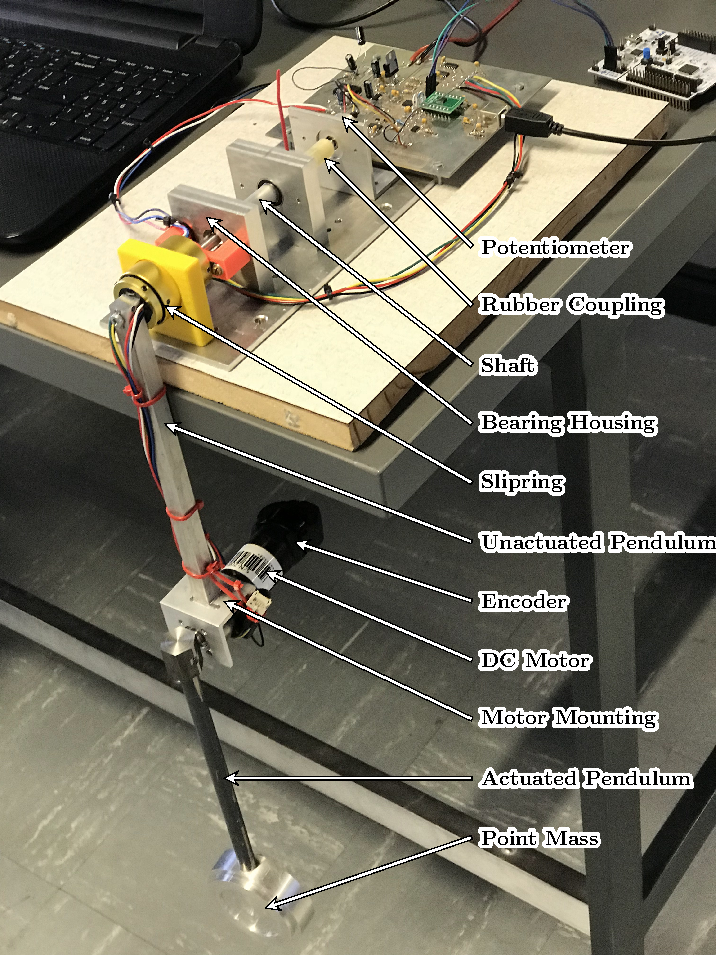
\includegraphics{./figs/mech_layout/mech_layout.pdf}
	\caption{Mechanical Hardware}
	\label{fig:mech_layout}
\end{figure}
%WHAT you are going to present in this chapter/section
%WHY you are presenting it, and
%HOW you are going to present it
The mechanical system was designed to practically demonstrate the feedback controllers to swing and balance the robotic gymnast in the future. The mechanical system will be presented by discussing the various components required to be implemented and mechanical characteristics.\\

It is important that the physical model holds the assumption made during the derivation of the robotic gymnast. These assumptions include planar dynamics of the robotic gymnast and rigid body dynamics. The assumption of rigid body dynamics were easily met due to the forces acting on the pendulums results in negligible strain and thus elongation can be ignored. The assumption of planar dynamics comes in affect with the connection between the rotating shaft and the unactuated pendulum. If the assumption holds there should be no vibration of the pendulum in any other direction than the rotating plane. This assumption holds in the mechanical system due to four screws used to keep the unactuated pendulum perpendicular to the shaft. \\

\subsection{Assembly}
Figure \ref{fig:mech_layout} emphasises important components that are discussed in the following section and explains their significance of use.\\	

The electrical slipring converts the rotating wires that leads to the motor mounted on the unactuated pendulum to stationary wires allowing for free rotation and easy connection to the electrical design.\\

The bearing housing holds the ball-bearings in place ensuring for no vibration and misalignment. These ballbearings were press-fitted into the housing, ensuring a secure connection.\\

The potentiometer's shaft is connected to the shaft by means of a rubber tube. The rubber tube was chosen as it easily connects and allows for misalignment. The delay of measurement due to elasticity of the rubber is negligible due to the system experiencing low acceleration. \\


\subsection{Structural Force Analysis}
%WHAT you are going to present in this chapter/section
%WHY you are presenting it, and
%HOW you are going to present it
The stress analysis of the rotating shaft is presented to provide the reader confidence in the shaft design. It will be presented by calculating the static yield safety factor and discussing whether the safety factor is sufficient.\\

The shaft was analysed as a 3 point supported beam shown in Figure \ref{fig:supp_beam} with a constant diameter throughout, using the smallest diameter in the design. The forces acting on the beam is the torque $T$ due to the rotating pendulums, and the normal force $F$ due the centripetal force of rotation and weight of the pendulums.\\

The normal force $F$ was selected as $\SI{25}{\newton}$ and the torque as $T = \SI{0.5}{Nm}$. These values were selected based of the simulation results that represent the worst conditions on the previous model.


\begin{figure}[h]
	\centering
	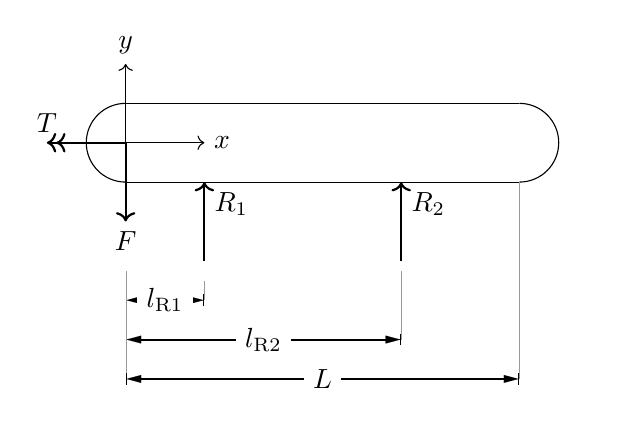
\begin{tikzpicture}[scale=0.5]




\begin{scope}
\clip [rotate=0] (-2,2) rectangle (0,-2);
\draw (0,0) circle [radius=1cm];
\end{scope}

\coordinate (O) at (0,0) ;
% Second cirle middle point
\coordinate (A) at (3.5,-6.06217); 
\coordinate (B) at (3.5+6.06217,-6.06217-3.5);
\coordinate (L1) at (10,0);

	% Lenght of pendulums are 7cm

	% Axis for underactuated Pendulum
	\draw[->] (0,0) -- (2,0) node[anchor=west] {$x$};
	\draw[->] (0,0) -- (0,2) node[anchor=south] {$y$};
	\draw[dashed] (0,0) -- (0,-2);
	
	%%%%%%%%%%%%%%%%%%%%%%%%%%%%%%%%%%%%%%%%%%%%%%%%%%%%%%%%%%%%%%%%%%%%%%%%%%%%%%

	%%%%%%%%%%%%%%%%%%%%%%%%%%%%%%%%%%%%%%%%%%%%%%%%%%%%%%%%%%%%%%%%%%%%%%%%%%%%%%
	
	%%%%%%%%%%%%%%%%%%%%%%%%%%%%%%%%%%%%%%%%%%%%%%%%%%%%%%%%%%%%%%%%%%%%%%%%%%%%%%
				%% Middle line for underactuated pendulum %%
	%\draw[dashed] (O) -- ([yshift=-4cm]L2);
	%%%%%%%%%%%%%%%%%%%%%%%%%%%%%%%%%%%%%%%%%%%%%%%%%%%%%%%%%%%%%%%%%%%%%%%%%%%%%%
	
		
	%%%%%%%%%%%%%%%%%%%%%%%%%%%%%%%%%%%%%%%%%%%%%%%%%%%%%%%%%%%%%%%%%%%%%%%%%%%%%%

	%%%%%%%%%%%%%%%%%%%%%%%%%%%%%%%%%%%%%%%%%%%%%%%%%%%%%%%%%%%%%%%%%%%%%%%%%%%%%%

	%Long lines for Beam
	\draw[] (0,1) -- ([yshift=1cm]L1);
	\draw[] (0,-1) -- 	([yshift=-1cm]L1);	
	
	%%%%%%%%%%%%%%%%%%%%%%%%%%%%%%%%%%%%%%%%%%%%%%%%%%%%%%%%%%%%%%%%%%%%%%%%%%%%%%
	%% Circle at the right %%
	
	\begin{scope}
	\clip [rotate=0] ([yshift=-2cm]L1) rectangle ([xshift=2cm,yshift=2cm]L1);
	\draw (L1) circle [radius=1cm];
	\end{scope}
	
	%% Reaction Forces
	\draw[->,thick] ([xshift=-8cm,yshift=-3cm]L1) -- ([xshift=-8cm,yshift=-1cm]L1) node[below right]{$R_{1}$};
	\draw[->,thick] ([xshift=-3cm,yshift=-3cm]L1) -- ([xshift=-3cm,yshift=-1cm]L1) node[below right]{$R_{2}$};
	
	%% Applied Forces
	\draw[->,thick] (0,0) -- (0,-2) node[below]{$F$};
	\draw[->>,thick] (0,0) -- (-2,0)node[above]{$T$};
	
						%% Dimensions of Beam %%
	\dimline[line style = {line width=0.7},extension start length=-0.25, extension end length=-0.25]{(0,-4)}{(2,-4)}{$l_{\text{R1}}$}
	
	\dimline[line style = {line width=0.7},extension start length=-0.25, extension end length=-0.25]{(0,-5)}{(7,-5)}{$l_{\text{R2}}$}
	
	\dimline[line style = {line width=0.7},extension start length=-0.25, extension end length=-0.5]{(0,-6)}{(10,-6)}{$L$}
	




	
\end{tikzpicture}
	\caption{Model of Rotating Shaft as a Simplified Beam}
	\label{fig:supp_beam}
\end{figure}

The beam is a static undetermined and was solved using the principle of superposition \citep{shigley1}. This results in the reaction forces shown in equations (\ref{eq:reactionForce1}), (\ref{eq:reactionForce2}) and (\ref{eq:reactionForce3}). 

\begin{equation} \label{eq:reactionForce1}
R_{1} = \SI{-17.045}{\newton}
\end{equation}
\begin{equation} \label{eq:reactionForce2}
R_{2} = \frac{ 8Fl_{1}[l_{3}^2 - l_{2}^2] }{l_{3}[4l_{2}^2-3l_{3}^2] } = \SI{20.45}{\newton}
\end{equation}
\begin{equation} \label{eq:reactionForce3}
R_{3} = \SI{21.59}{\newton}
\end{equation}

The maximum bending stress occurs at $x=\SI{0.085}{\meter}$ and the maximum torsion stress at $x=\SI{0}{\meter}$. The safety factor of yielding will be determined at these two positions.\\

Equations (\ref{eq:torsionForce}) and (\ref{eq:axialForce}) are used to determine the maximum stresses at these two points and using the Mohr circle the principle stresses are determined.  These stresses are shown in Table \ref{table:stresses}.\\


\begin{table}[]
	\centering
	\begin{tabular}{|c|c|c|}
		\hline
		Stresses & $x = \SI{0}{\meter}$ & $x=\SI{0.085}{\meter}$ \\
		\hline
		\hline
		$\sigma_{f_{1}}$ & $\SI{300}{kPa}$ & $\SI{282}{kPa}$ \\
		\hline
		$\sigma_{f_{2}}$ & $\SI{0}{kPa}$& $\SI{-245}{kPa}$ \\
		\hline
		$\sigma_{f_{3}}$ & $\SI{0}{Pa}$& $\SI{0}{Pa}$ \\
		\hline
		$\tau_{f}$ & $\SI{300}{kPa}$&$\SI{263}{kPa}$  \\
		\hline
		$M_{max}$ & $\SI{0}{Nm}$&$\SI{-0.2899}{Nm}$ \\
		\hline
	\end{tabular}
	\caption{Stresses Developed in Shaft}
	\label{table:stresses}
\end{table}

The conservative Von Mises theory shown in equation (\ref{eq:vonMises}) was used to determine the safety factor on static yielding, where $S_{y}$ is the yield stress of extruded aluminium and is $\SI{290}{MPa}$. The minimum safety factor on static yielding occurred at $x=\SI{0.085}{\meter}$ and was calculated as 634. This shows the loads will be no problem for the shaft.\\

Fatigue due to cyclic loads were ignored due the shaft not rotating more than a 1000 times and the safety factor on static yielding  on a conservative model is sufficient.

\begin{equation} \label{eq:axialForce}
\sigma_{f} = \frac{M\cdot r}{I_{m}}
\end{equation}

\begin{equation} \label{eq:torsionForce}
\tau_{f} = \frac{T\cdot r}{J} + \frac{4F_{max}}{3A}
\end{equation}


\begin{equation} \label{eq:vonMises}
n_{s} = \frac{S_{y}}{\sqrt{\frac{(\sigma_{f_{1}}-\sigma_{f_{2}})^2+(\sigma_{f_{2}}-\sigma_{f_{3}})^2+(\sigma_{f_{3}}-\sigma_{f_{1}})^2}{2}}}
\end{equation}

\subsection{Inertia of Pendulums}
\begin{figure}[h]
	\centering
	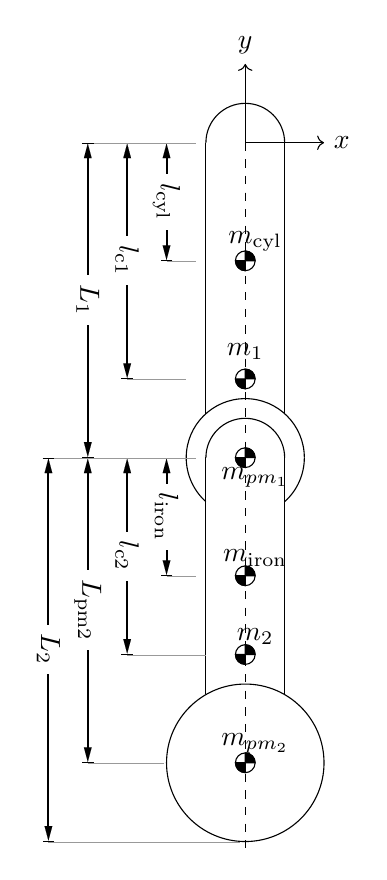
\begin{tikzpicture}[scale=0.5]




\begin{scope}
\clip [rotate=0] (-2,0) rectangle (2,2);
\draw (0,0) circle [radius=1cm];
\end{scope}

\coordinate (O) at (0,0) ;
% Second cirle middle point
\coordinate (A) at (3.5,-6.06217); 
\coordinate (B) at (3.5+6.06217,-6.06217-3.5);
\coordinate (L1) at (0,-6);
\coordinate (L2) at (0,-14);
\coordinate (x) at (0,-2);
\coordinate (AA) at ([xshift=-1cm]x);
\coordinate (BB) at ([xshift=1cm]x);
\coordinate (CC) at ([xshift=1cm,yshift=-1.5cm]x);
\coordinate (DD) at ([xshift=-1cm,yshift=-1.5cm]x);

% Lenght of pendulums are 7cm

% Axis for underactuated Pendulum
\draw[->] (0,0) -- (2,0) node[anchor=west] {$x$};
\draw[->] (0,0) -- (0,2) node[anchor=south] {$y$};
\draw[dashed] (0,0) -- (0,-2);

%%%%%%%%%%%%%%%%%%%%%%%%%%%%%%%%%%%%%%%%%%%%%%%%%%%%%%%%%%%%%%%%%%%%%%%%%%%%%%

%%%%%%%%%%%%%%%%%%%%%%%%%%%%%%%%%%%%%%%%%%%%%%%%%%%%%%%%%%%%%%%%%%%%%%%%%%%%%%

%%%%%%%%%%%%%%%%%%%%%%%%%%%%%%%%%%%%%%%%%%%%%%%%%%%%%%%%%%%%%%%%%%%%%%%%%%%%%%
%% Middle line for underactuated pendulum %%
\draw[dashed] (O) -- ([yshift=-4cm]L2);
%%%%%%%%%%%%%%%%%%%%%%%%%%%%%%%%%%%%%%%%%%%%%%%%%%%%%%%%%%%%%%%%%%%%%%%%%%%%%%


%%%%%%%%%%%%%%%%%%%%%%%%%%%%%%%%%%%%%%%%%%%%%%%%%%%%%%%%%%%%%%%%%%%%%%%%%%%%%%
%% Dimensions of underactuated Pendulum %%
\dimline[line style = {line width=0.7},extension start length=-0.25, extension end length=-0.25]{(-2,0)}{(-2,-3)}{$l_{\text{cyl}}$}

\dimline[line style = {line width=0.7},extension start length=-0.25, extension end length=-0.25]{(-3,0)}{(-3,-6)}{$l_{\text{c1}}$}

\dimline[line style = {line width=0.7},extension start length=-0.25, extension end length=-0.25]{(-4,0)}{(-4,-8)}{$L_{1}$}

%%%%%%%%%%%%%%%%%%%%%%%%%%%%%%%%%%%%%%%%%%%%%%%%%%%%%%%%%%%%%%%%%%%%%%%%%%%%%%

%Long lines for underactuated pendulum
\draw[] (-1,0) -- ([xshift=-1cm,yshift=-0.9cm]L1);
\draw[] (1,0) -- 	([xshift=1cm,yshift=-0.9cm]L1);	



%%%%%%%%%%%%%%%%%%%%%%%%%%%%%%%%%%%%%%%%%%%%%%%%%%%%%%%%%%%%%%%%%%%%%%%%%%%%%%
%% smaller Middle circle for both pendulums %
\begin{scope}
\clip ([xshift=-1.2cm,yshift=-2cm]L1) rectangle ([xshift=1.2cm,yshift=2cm]L1);
\draw ([yshift=-2cm]L1) circle [radius=1cm];
\end{scope}


% Bigger Middler Circle for both pendulums
%\draw ([yshift=-2cm]L1) circle [radius=1.5cm];
\draw[] ([xshift=1.5cm,yshift=-2cm]L1)
arc[start angle = 0, end angle = 228, radius = 1.5cm];

\draw[] ([xshift=1.5cm,yshift=-2cm]L1)
arc[start angle = 0, end angle =-48 , radius = 1.5cm];

%\draw [rotate=00] (0.866+3.5,0.5-6.06217+2) rectangle (-0.866+3.5-2,-0.5-6.06217);

%%%%%%%%%%%%%%%%%%%%%%%%%%%%%%%%%%%%%%%%%%%%%%%%%%%%%%%%%%%%%%%%%%%%%%%%%%%%%%

\begin{scope}
\clip ([xshift=-1.5cm,yshift=-2cm]L1) rectangle ([xshift=1.5cm,]L2);
\draw[] ([xshift=-1cm,yshift=-1.5cm]L1) --([xshift=-1cm]L2);
\draw[]([xshift=1cm,yshift=-1.5cm]L1) --([xshift=1cm,]L2);
\end{scope}


%%%%%%%%%%%%%%%%%%%%%%%%%%%%%%%%%%%%%%%%%%%%%%%%%%%%%%%%%%%%%%%%%%%%%%%%%%%%

%%%%%%%%%%%%%%%%%%%%%%%%%%%%%%%%%%%%%%%%%%%%%%%%%%%%%%%%%%%%%%%%%%%%%%%%%%%%%%

%%%%%%%%%%%%%%%%%%%%%%%%%%%%%%%%%%%%%%%%%%%%%%%%%%%%%%%%%%%%%%%%%%%%%%%%%%%%%%
%% Dimensions of actuated Pendulum %%
\dimline[line style = {line width=0.7},extension start length=-0.25, extension end length=-0.25]{(-2,-8)}{(-2,-11)}{$l_{\text{iron}}$}

\dimline[line style = {line width=0.7},extension start length=-0.25, extension end length=-0.4]{(-3,-8)}{(-3,-13)}{$l_{\text{c2}}$}

\dimline[line style = {line width=0.7},extension start length=-0.25, extension end length=-0.25]{(-4,-8)}{(-4,-15.75)}{$L_{\text{pm2}}$}


\dimline[line style = {line width=0.7},extension start length=-0.25, extension end length=-0.5]{(-5,-8)}{(-5,-17.75)}{$L_{2}$}
%%%%%%%%%%%%%%%%%%%%%%%%%%%%%%%%%%%%%%%%%%%%%%%%%%%%%%%%%%%%%%%%%%%%%%%%%%%%%%


%%%%%%%%%%%%%%%%%%%%%%%%%%%%%%%%%%%%%%%%%%%%%%%%%%%%%%%%%%%%%%%%%%%%%%%%%%%%%%
%% Circle at the bottom %%
\draw ([yshift=-1.75cm]L2) circle [radius=2cm];
%%%%%%%%%%%%%%%%%%%%%%%%%%%%%%%%%%%%%%%%%%%%%%%%%%%%%%%%%%%%%%%%%%%%%%%%%%%%%%


%%%%%%%%%%%%%%%%%%%%%%%%%%%%%%%%%%%%%%%%%%%%%%%%%%%%%%%%%%%%%%%%%%%%%%%%%%%%%%


%%%%%%%%%%%%%%%%%%%%%%%%%%%%%%%%%%%%%%%%%%%%%%%%%%%%%%%%%%%%%%%%%%%%%%%%%%%%%%
%% Centroid symbol for underactuade pendulum %%
\draw (0,-6) circle [radius=0.25cm];
\draw (0,-6-0.25) -- (0,-6+0.25)  node[above]{$m_{1}$};`
\draw (0,-6+0.25) -- (0,-6-0.25);
\filldraw[fill=black,draw=black] (0,-6) -- (0.25,-6)
arc[start angle = 0, end angle = 90, radius = 0.25] -- cycle;

\filldraw[fill=black,draw=black] (0,-6) -- (-0.25,-6)
arc[start angle = 180, end angle = 270, radius = 0.25] -- cycle ;
%%%%%%%%%%%%%%%%%%%%%%%%%%%%%%%%%%%%%%%%%%%%%%%%%%%%%%%%%%%%%%%%%%%%%%%%%%%%%%

%%%%%%%%%%%%%%%%%%%%%%%%%%%%%%%%%%%%%%%%%%%%%%%%%%%%%%%%%%%%%%%%%%%%%%%%%%%%%%
%% Centroid symbol for actuaded pendulum %%
\draw (0,-13) circle [radius=0.25cm];
\draw (-0.25,-13) -- (0.25,-13)  node[above]{$m_{2}$};
\draw (0,-13+0.25) -- (0,-13-0.25);
\filldraw[fill=black,draw=black] (0,-13) -- (0.25,-13)
arc[start angle = 0, end angle = 90, radius = 0.25] -- cycle;

\filldraw[fill=black,draw=black] (0,-13) -- (-0.25,-13)
arc[start angle = 180, end angle = 270, radius = 0.25] -- cycle ;
%%%%%%%%%%%%%%%%%%%%%%%%%%%%%%%%%%%%%%%%%%%%%%%%%%%%%%%%%%%%%%%%%%%%%%%%%%%%%%
%% Centroid symbol for pointmass 2 %%
\draw (0,-15.75) circle [radius=0.25cm];
\draw (-0.25,-15.75) -- (0.25,-15.75)  node[above]{$m_{\text{$pm_2$}}$};
\draw (0,-15.75+0.25) -- (0,-15.75-0.25);
\filldraw[fill=black,draw=black] (0,-15.75) -- (0.25,-15.75)
arc[start angle = 0, end angle = 90, radius = 0.25] -- cycle;

\filldraw[fill=black,draw=black] (0,-15.75) -- (-0.25,-15.75)
arc[start angle = 180, end angle = 270, radius = 0.25] -- cycle ;
%%%%%%%%%%%%%%%%%%%%%%%%%%%%%%%%%%%%%%%%%%%%%%%%%%%%%%%%%%%%%%%%%%%%%%%%%%%%%%
%% Centroid symbol for pointmass 1 %%
\draw (0,-8) circle [radius=0.25cm];
\draw (-0.25,-8) -- (0.25,-8)  node[below]{$m_{\text{$pm_{1}$}}$};
\draw (0,-8+0.25) -- (0,-8-0.25);
\filldraw[fill=black,draw=black] (0,-8) -- (0.25,-8)
arc[start angle = 0, end angle = 90, radius = 0.25] -- cycle;

\filldraw[fill=black,draw=black] (0,-8) -- (-0.25,-8)
arc[start angle = 180, end angle = 270, radius = 0.25] -- cycle ;
%%%%%%%%%%%%%%%%%%%%%%%%%%%%%%%%%%%%%%%%%%%%%%%%%%%%%%%%%%%%%%%%%%%%%%%%%%%%%%
%% Centroid symbol for cylinder %%
\draw (0,-3) circle [radius=0.25cm];
\draw (-0.25,-3) -- (0.25,-3)  node[above]{$m_{\text{cyl}}$};
\draw (0,-3+0.25) -- (0,-3-0.25);
\filldraw[fill=black,draw=black] (0,-3) -- (0.25,-3)
arc[start angle = 0, end angle = 90, radius = 0.25] -- cycle;

\filldraw[fill=black,draw=black] (0,-3) -- (-0.25,-3)
arc[start angle = 180, end angle = 270, radius = 0.25] -- cycle ;
%%%%%%%%%%%%%%%%%%%%%%%%%%%%%%%%%%%%%%%%%%%%%%%%%%%%%%%%%%%%%%%%%%%%%%%%%%%%%%
%% Centroid symbol for iron ron %%
\draw (0,-11) circle [radius=0.25cm];
\draw (-0.25,-11) -- (0.25,-11)  node[above]{$m_{\text{iron}}$};
\draw (0,-11+0.25) -- (0,-11-0.25);
\filldraw[fill=black,draw=black] (0,-11) -- (0.25,-11)
arc[start angle = 0, end angle = 90, radius = 0.25] -- cycle;

\filldraw[fill=black,draw=black] (0,-11) -- (-0.25,-11)
arc[start angle = 180, end angle = 270, radius = 0.25] -- cycle ;



\end{tikzpicture}
	\caption{Simplified Drawing of Physical Model}
	\label{fig:model_drawing}
\end{figure}

Figure \ref{fig:model_drawing} shows a functional drawing of the physical model in order to aid the reader visually in understanding how the inertia of the system was determined. In equation (\ref{eq:condense1}) and (\ref{eq:condense2}) the $I_{a}$ and $I_{b}$ represents the inertia of the unactuated and actuated pendulum about the axis coming out of the page passing through their center of mass respectively.\\

Each pendulum contains parts that contribute to the pendulum's inertia due to each part representing a different physical form. How the inertia values shown in Table \ref{table:system_param} were determined will be shown below with the physical system parameters shown in the Table \ref{table:model_param}\\

The actuated pendulum consist out of an aluminium square rod connected to the shaft and the motor mounting. The inertia of a square rod through it's center of mass is: $$ I_{cyl} = \frac{1}{12}m_{cyl}[w^2+L^2_{1}]$$

The motor, gearbox and the motor mount was viewed as a point mass. Its inertia around the center of mass of the unactuated pendulum is: $$I_{pointmass_1} = m_{pointmass_1}\cdot[L_{1}-l_{c1}]^2 $$

The total inertia of the unactuated pendulum around its center of mass is: $$ I_{a} =I_{pointmass_1} +  I_{cyl} + m_{cyl}\cdot[l_{c2}-l_{cyl}]^2 $$ where the parallel axis theorem was used to move the aluminium rod's inertia to the center of mass of the unactuated pendulum.

The actuated pendulum contains similar parts as the unactuated pendulum: a pointmass at the bottom and an iron rod connected to the motor shaft. Determining the inertia of the actuated pendulum is thus exactly the same as the unactuated pendulum.\\

During the simulation it was noticed that the ratio between the unactuated and actuated pendulum $\frac{I_{b}}{I_{a}}$ should be 1 or greater for the swing-up controller to bring the robotic gymnast to the unstable equilibrium position in a feasible time frame. This is the reason adding another pointmass to the actuated pendulum to compensate for the inertia the motor creates.


\begin{table}[]
	\centering
	\begin{tabular}{|c|c|c|c|}
		\hline
		Unactuated Pendulum& Value & Actuated Pendulum & Value \\
		\hline
		\hline
		$m_{\text{cyl}}$ & \SI{0.1443}{\kilogram} & $m_{\text{iron}}$ & \SI{0.257}{\kilogram} \\
		\hline
		$w_{\text{cyl}}$ & \SI{12}{mm}& $w_{\text{iron}}$& \SI{12}{mm} \\
		\hline
		$m_{\text{pointmass1}}$ & \SI{0.432}{\kilogram}& $m_{\text{pointmass2}}$& \SI{0.306}{\kilogram}\\
		\hline
		$l_{\text{cyl}}$ & \SI{0.235}{\meter}& $l_{\text{iron}}$& \SI{0.223}{\meter} \\
		\hline
		$L_{\text{c1}}$ & \SI{0.2056}{\meter} & $L_{\text{c2}}$& \SI{0.1940}{\meter}\\
		\hline
		$L_{1}$ & \SI{0.235}{\meter}& $L_{2}$& \SI{0.303}{\meter} \\
		\hline
	\end{tabular}
	\caption{Physical Model Paramaters}
	\label{table:model_param}
\end{table}

\subsection{Center of Mass}
Each pendulum can be seen as a system containing discrete components, where each component center of mass is easily identified. Both iron rod and aluminium rod center of mass is in the middle of their rod lenght and the rest are seen as point masses. However each of these components center of mass contribute to the center of mass of each pendulum.\\

The center of mass for each pendulum from their hinge of rotation shown in Table \ref{table:centerOfMass} was calculated using equation (\ref{eq:centerOfMass}). 

\begin{equation} \label{eq:centerOfMass}
\vec{\boldmath{r}} = \frac{\sum_{i}^{j}r_{i}m_{i}}{\sum_{i}^{j}m_{i}}
\end{equation}

Where $r$ is the lenght to the center of mass for each $m$ discrete component from the their hinge of rotation.

\begin{table}[]
	\centering
	\begin{tabular}{|c|c|}
		\hline
		Pendulum & Center of Mass [\SI{}{m}] \\
		\hline
		\hline
		Unactuated  & \SI{0.2056}{} \\
		\hline
		Actuated  & \SI{0.1940}{} \\
		\hline
	\end{tabular}
	\caption{Center of Mass for Each Pendulum from their Rotating Hinge}
	\label{table:centerOfMass}
\end{table}


\subsection{Motor}
The chosen motor used during experiments was the \textit{Faulhaber DC 3257 012 CR} micromotor. It was used in combination with the \textit{Faulhaber Planetary Gearhead 32/3} Series. The gearbox is a 2 stage reduction gearbox with an overall rounded reduction ratio of 14:1. The motor is capable of providing a stall torque of \SI{539}{mNm} which is a converted output torque from the gearbox of \SI{7.646}{Nm}.\\

The motor terminal connection is connected directly to the PCB of the electronic design being routed through the slipring. The motor assembly contains an encoder for position measurements and it's signal and power connection is also routed through the slipring and connected to the PCB seen in Figure \ref{fig:mech_layout}\\

\section{Electronic Hardware}
\label{sec:electronic_hardware}
\begin{figure}[h]
	\centering
	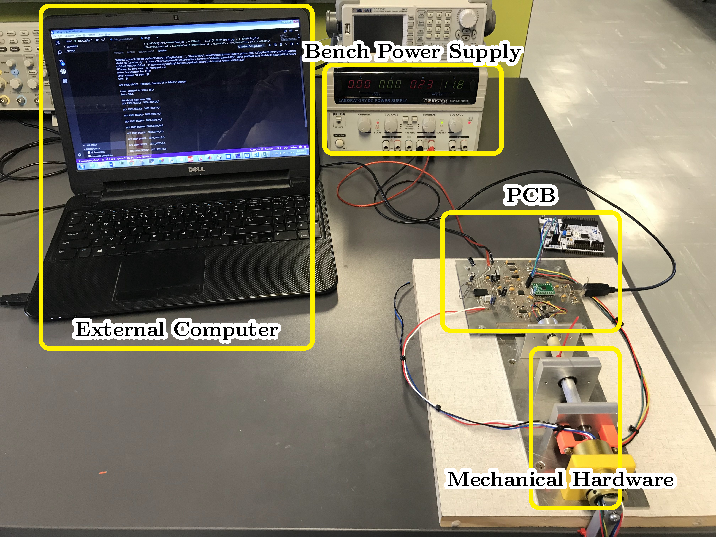
\includegraphics{./figs/elec_sys/elec.pdf}
	\caption{Electronic Hardware Setup}
	\label{fig:elec_sys}
\end{figure}
%WHAT you are going to present in this chapter/section
%WHY you are presenting it, and
%HOW you are going to present it
The electronic hardware shown in Figure \ref{fig:elec_sys} was a crucial component for the successful implementation of the robotic gymnast. The electronic design provided the means to determine the system characteristics and verification of the simulated model. It will be presented by discussing the various components implemented to achieve the results in this report.

\subsection{System Description}

\begin{figure}[h]
	\centering
	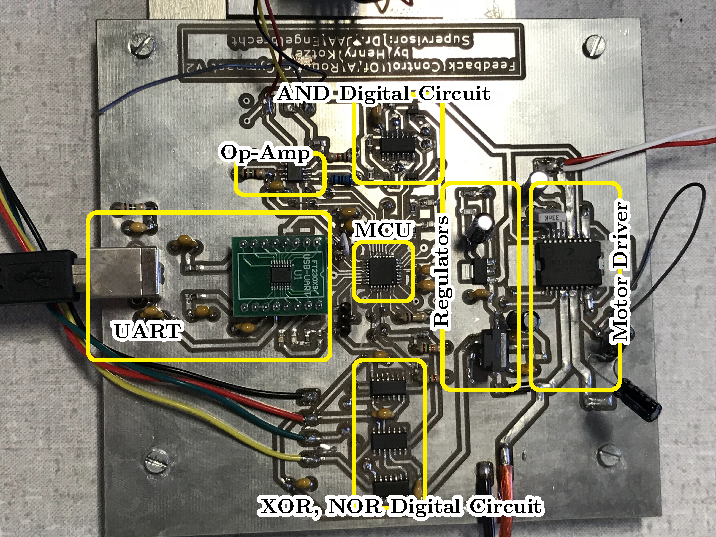
\includegraphics{./figs/PCB_layout/PCB.pdf}
	\caption{PCB}
	\label{fig:pcb}
\end{figure}


% Show block diagram of the system and explain the functioning og the system
\begin{figure}[h]
	\centering
	\usetikzlibrary{shadows,arrows}
% Define the layers to draw the diagram
\pgfdeclarelayer{background}
\pgfdeclarelayer{foreground}
\pgfsetlayers{background,main,foreground}

% Define block styles  
\tikzstyle{block}=[draw, fill=blue!20, text width=7.0em, text centered,
minimum height=1.5em,drop shadow]
\tikzstyle{blocks} = [block, rounded corners, drop shadow]
\tikzstyle{texto} = [above, text width=6em, text centered]
\tikzstyle{linepart} = [draw, thick, color=black!50, -latex', dashed]
\tikzstyle{line} = [draw, thick, color=black!50, -latex']
\tikzstyle{ur}=[draw, text centered, minimum height=0.01em]

% Define distances for bordering
\newcommand{\blockdist}{1.3}
\newcommand{\edgedist}{1.5}

\newcommand{\external}[2]{node (e#1) [blocks]
	{External 12V Supply\\{\scriptsize\textit{#2}}}}

\newcommand{\regulator}[2]{node (r#1) [blocks]
	{Voltage Regulation\\{\scriptsize\textit{#2}}}}

\newcommand{\uC}[2]{node (uC#1) [blocks]
	{$\mu$Controller\\{\scriptsize\textit{#2}}}}

\newcommand{\uart}[2]{node (uart#1) [blocks]
	{PC UART Interface\\{\scriptsize\textit{#2}}}}

\newcommand{\prog}[2]{node (prog#1) [blocks]
	{Programming / Debug Interface\\{\scriptsize\textit{#2}}}}

\newcommand{\motor}[2]{node (motor#1) [blocks]
	{Motor\\{\scriptsize\textit{#2}}}}

\newcommand{\sigcond}[2]{node (sigcond#1) [blocks]
	{Signal Conditioning\\{\scriptsize\textit{#2}}}}

\newcommand{\encdig}[2]{node (encdig#1) [blocks]
	{Digital Logic Circuit\\{\scriptsize\textit{#2}}}}

\newcommand{\pc}[2]{node (pc#1) [blocks]
	{PC\\{\scriptsize\textit{#2}}}}

\newcommand{\physical}[2]{node (physical#1) [blocks]
	{Physical Model\\{\scriptsize\textit{#2}}}}

\newcommand{\motordriver}[2]{node (motordriver#1) [blocks]
	{Motor Driver\\{\scriptsize\textit{#2}}}}

\newcommand{\digitlogic}[2]{node (digitlogic#1) [blocks]
	{Digital Logic Circuit\\{\scriptsize\textit{#2}}}}

\newcommand{\encoder}[2]{node (encoder#1) [blocks]
	{Hall Effect Encoder\\{\scriptsize\textit{#2}}}}
% Draw background
\newcommand{\background}[5]{%
	\begin{pgfonlayer}{background}
		% Left-top corner of the background rectangle
		\path (#1.west |- #2.north)+(-0.5,0.5) node (a1) {};
		% Right-bottom corner of the background rectanle
		\path (#3.east |- #4.south)+(+0.5,-0.25) node (a2) {};
		% Draw the background
		\path[fill=yellow!20,rounded corners, draw=black!50, dashed]
		(a1) rectangle (a2);
		\path (a1.east |- a1.south)+(0.8,-0.3) node (u1)[texto]
		{\scriptsize\textit{Unidad #5}};
\end{pgfonlayer}}

\newcommand{\transreceptor}[3]{%
	\path [linepart] (#1.east) -- node [above]
	{\scriptsize Transreceptor #2} (#3);}


\begin{tikzpicture}[scale=0.7,transform shape]

% Draw diagram elements
\path \external {1}{DC Power Supply};
\path (e1.east)+(2.0,0.0) \physical{1}{Potentiometer};
\path (e1.south)+(0.0,-1.5) \regulator{1}{5V, 3.3V};
\path (r1.south)+(0.0,-1.5) \uC{1}{ARM M0 STM32F030C6};

% PC 
\path (e1.west)+(-2.5,0) \pc{1}{};

% PC UART Interface
\path (r1.west)+(-6,0) \uart{1}{FT230XS};

%Programming/Debug Interface
\path (r1)+(-4.05,0) \prog{1}{Serial Wire Debug};

%Signal Conditioning
\path (uC1.east)+(2.0,0) \sigcond{1}{OPA342 OpAmp};

%JK Flipflops
\path (uC1.west)+(-2.0,-3.0) \encdig{1}{J-K Flipflop \& Nor's};

% Motor
\path (uC1.south) + (0,-5) \motor{1}{DC Brushed Motor};

% Digital Logic: Logic Level Convertes
\path (uC1.south) + (0,-2) \digitlogic{1}{Logic Level Converters \&  Direction Control};

% Motor Driver
\path (digitlogic1.east)+(2.0,0) \motordriver{1}{MC33887};

%Hall Effect Enconder
\path (encdig1.south)+ (0,-1.8) \encoder{1}{Mounted On Motor};




% Draw arrows between elements
\path [line] (e1.south) -- node [above] {} (r1);
\path [line] (r1.south) -- node [above] {} (uC1);

% uC to UART
\path [line] (uC1.west) -| node [below] {} (uart1);

% uC to Programming/Debug Interface
\path [line] (uC1.west)+(0,0.2) -| node [below]{}(prog1); 

% JK FlipFlops
%\path [line] (uC1.west)+(0,-0.2) -| node [above]{}(encdig1); 

\draw[->] (encdig1) |- ([yshift=-0.2cm]uC1.west);


\path [line] (sigcond1.west) -- node[right]{}(uC1);

\path [line] (physical1.south) -- node[above]{}(sigcond1);

% Motor Driver to signal Conditioning
\path [line] (motordriver1.north) -- node[below]{}(sigcond1);

% PC UART Interface -> PC
\path [line] (uart1.north) |- node[left]{}(pc1);

% Programming/Debug Interfac -> PC
\path [line] (prog1.north) -- node[below]{}(pc1);

% Motor Driver -> Motor
\path [line] (motordriver1.south) |- node[right]{}(motor1); 

% Microcontroller -> Digitical logic
\path [line] (uC1.south) -- node[above]{}(digitlogic1);

\path [line] (digitlogic1.east) -- node[left]{}(motordriver1);


\path [line] (encoder1.north) -- node[below]{}(encdig1);


\path [line] (motor1.west) -- node[right]{}(encoder1);

\begin{pgfonlayer}{background}
\path (uart1.west -| physical1.east) node (a) {};
\path (motor1.south -| physical1.south)+(+0.5,-0.3) node (b) {};
\path (digitlogic1.south |- motor1.east)+(+0.5,0.5) node (c) {};

\path[fill=yellow!20,rounded corners, draw=black!50, dashed]
([xshift=-0.5cm,yshift=1cm]uart1.west) rectangle ([xshift=0.5cm,yshift=-2cm]motordriver1.east);           
\path (digitlogic1.north west)+(-0.2,0.2) node (a) {};

\end{pgfonlayer}

\path ([xshift=-4.5cm,yshift=-0.5cm]encdig1.south) node (meep) {PCB Boundary};

%\path (wa.south)+(0,-\blockdist/5) node (meep) {System Boundary};


\end{tikzpicture}
	\caption{Electronic System Overview}
	\label{fig:electronicSystemOverview}
\end{figure}



Figure \ref{fig:pcb} shows the manufacured PCB and Figure \ref{fig:electronicSystemOverview} provides a system overview of how the different subsystems functions together and what inputs are outside from the PCB design. A brief overview of the interfaces between these subsystems are provided in the following section.\\

The micro-controller receives the different signals that has been correctly conditioned from supporting circuitry to interpret the dynamics of the system. From these signals it is able to output the correct signals to instruct the next command.\\

The digital logic circuit that consist out of logic level converters receives a signal from the microcontroller and performs signal conditioning to interface with the motor driver and determines the correct direction to rotate the motor. \\

The motor driver controls the DC brushed motor based of the digital signals and provides a proportional feedback current that is delivered to the unity-gain amplifier.\\

The motor contains an encoder that indicates the direction and position of the rotor through digital signals that is sent through a digital logic decoder to retrieve only critical information from the encoded signals. \\

The physical model contains a potentiometer that measures the unactuated pendulum's angle and this signal is sent to the unity-gain amplifier.\\

The microcontroller will use the Universal Asynchronous Receive Transmit (UART) interface as its data acquisition protocol to send the necessary information to the computer. \\

The micro-controller is programmed using the Serial Wire Debug (SWD) protocol to transfer the binaries from the computer.\\

Power is provided using a external 12V power-supply, which will provide power to the motor, but also using a regulator to down convert to a 5V and 3.3V to provide power to the microcontoller and the other peripherals.


\subsection{Microcontroller}
The microcontroller chosen is the STM32F030C6. The selection was done according to the ease of setting up, memory size, physical dimensions and the peripherals it provided. The selection is described below.\\

The STM32F030C6 is based on the ARM M0 architecture which is ARM's entry level microcontroller architecture. It requires little support circuitry to have a microcontroller which is fully  functioning with only the SWD protocol to program the chip.\\

It was difficult to determine the memory size specification for the project. This uncertainty ensured that the largest memory size the ARM M0 architecture could provide was selected.\\

The Electrical and Electronic Department's PCB manufacturing machine can only provide a  minimum track width of \SI{0.3}{mm}. This resulted in choosing a microcontroller which footprint would meet this requirement.\\

Based on the conceptual design, the chosen microcontroller was required to contain 2 ADC's channels, minimum of 5 GPIO's and 1 serial communication peripheral.\\

From these requirements and specification the STM32F030C6 was the best candidate to meet all of the above mentioned requirements.

\subsubsection{Programming / Debug Interface}
The \textit{Atollic TrueSTUDIO for ARM 8.0.0} Integrated Development Environment (IDE) was used for writing the source code which converts the source code to the Executable and Linkable Format (.elf) file. These .elf files is then written using the SWD protocol to the microcontroller. Debugging of the source code occurred using the same IDE which allows the programmer to inspect variables, timers and logic.

\subsubsection{PC UART Interface }

The purpose of the UART to serial communication was for the data acquisition of the system response, debugging and sending the control input that was computed on the external computer.\\

The external computer executed a Python script that was listening for any activity on the computer's driver port for information about the system. The Python script would react differently based on whether debugging, system identification tests or experiments occurred.\\

The UART to Serial chip used was the FT230x (USB to BASIC UART IC). It was chosen due to the easy support circuitry it requires with the option to use Light Emitting Diodes (LED) to indicate any activity on the receive (Rx)  \& transmit (Tx) communication lines.\\

The UART to serial circuit was tested by doing a loopback test. The loopback test consist of connecting the Tx and Rx lines together. This results in the circuit echoing anything that the receiver has sent. The schematic of the circuitry is shown in Appendix \ref{sec:schematics}.


\subsection{Voltage Regulation}

The various components used in the electronic design required different supply voltages and can be seen in Table \ref{table:supplyVoltage}.\\


\begin{table}[]
	\centering
	\begin{tabular}{|c|c|}
		\hline
		Component & Supply Voltage [\SI{}{V}] \\
		\hline
		\hline
		Digital Logic, Op-Amp \& Sensors & \SI{5}{} \\
		\hline
		Microcontroller & \SI{3.3}{} \\
		\hline
		Motor Driver & \SI{12}{} \\
		\hline
	\end{tabular}
	\caption{Suppy Voltage's for the Different Components}
	\label{table:supplyVoltage}
\end{table}

The \SI{12}{\volt} supply was provided using an external bench power-supply and were done converted to \SI{5}{V} and \SI{3.3}{V} using linear voltage regulators. The schematic for each voltage regulator is shown in Appendix \ref{sec:schematics}, and includes a LED to ensure the minimum load was met for each regulator. The LED also acts as a visual debugging method.

\subsection{Potentiometer Sensor}
\subsubsection{Principle of Operation}
\begin{figure}[h]
	\centering
		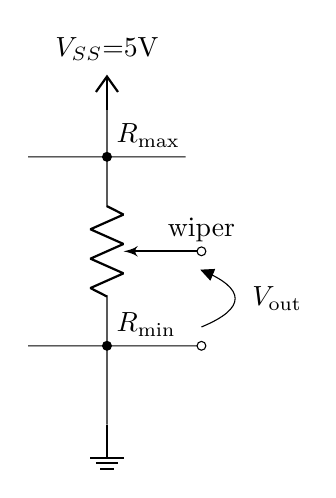
\begin{tikzpicture}[scale=2]
	
	
	\draw[color=black]
	(0,0) node[ground]{}
	
	(0,2) node[vcc]{$V_{SS}$=5V} 
	(0,2) to [short] (0,1.7) node[anchor=south west] {$R_{\text{max}}$}
	(0,1.7) to [pR,*-*] (0,0.5) node[anchor=south west] {$R_{\text{min}}$}
	(0,0.5) to [short] (0,0) 
	(-0.5,0.5) to [short] (0.6,0.5) 
	(0.5,1.7) to [short] (-0.5,1.7) 
	

	
	;
	
	\draw node[ocirc] (A) at (0.6,1.1) {};
	\draw node[ocirc] (B) at (0.6,0.5) {};
	\draw (B) to[open, v=$V_{\text{out}}$] (A);
	\draw (A) [thick]-- (0.2,1.1){};
	
	\draw (A) node[anchor=south] {wiper};
	
	
	
	
	
	\end{tikzpicture}
	\caption{Simplified Model of a Potentiometer}
	\label{fig:potentiometer}
\end{figure}
The rotary position potentiometer consist out of a wiper that is attached to a rotating shaft. This wiper moves across a internal resistor as the shaft rotates and changes the effective resistance across the output terminal. It provides thus a proportional voltage to its position as seen in Figure \ref{fig:potentiometer} that indicates the position.

\subsubsection{Interface}
\begin{figure}[h]
	\centering
	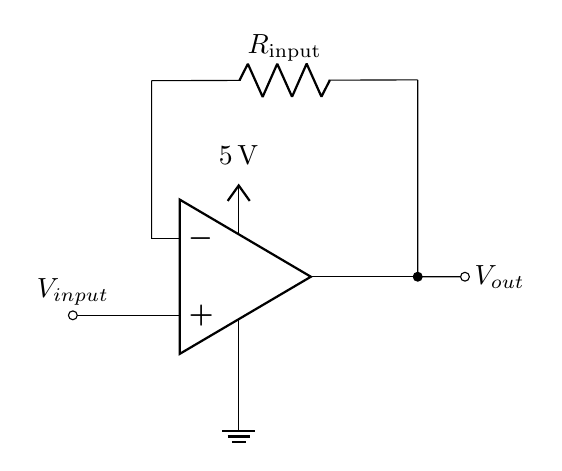
\begin{tikzpicture}[scale=2]


\draw (0,0) node[op amp] (opamp) {}
%(opamp.+) node[left] {$v_+$}
%(opamp.-) node[left] {$v_-$}
(opamp.up) --++(0,0.1) node[vcc]{5\,\textnormal{V}}
(opamp.down) --++(0,-0.5) node[ground]{};

\draw (opamp.out) to[short] ([xshift=0.5cm]opamp.out) node[anchor=south east]{};

\draw ([xshift=0.5cm]opamp.out) to[short] ([xshift=0.5cm,yshift=1.25cm]opamp.out)

([xshift=0.5cm]opamp.out) to[short,*-o ] ([xshift=0.8cm]opamp.out) node[anchor=west]{$V_{out}$}


([xshift=0.5cm,yshift=1.25cm]opamp.out) to[R,l_=$R_{\text{input}}$] ([yshift=1cm]opamp.-)

([yshift=1cm]opamp.-) to[short](opamp.-); 

\draw (opamp.+) to[short,-o] ([xshift=-0.5cm]opamp.+) node[anchor=south]{$V_{input}$}

;




\end{tikzpicture}
	\caption{Unity Gain Amplifier Circuit}
	\label{fig:unitygain}
\end{figure}
The signal produced by the rotary potentiometer varies from 4.95V and 50mV as it rotates from 360\textdegree \space to 0\textdegree. This signal was sent through a simple voltage divider circuit to reduce the signal to 3V and 15mV to be within the sampling limits of the microcontroller. The scaled voltage was then sent through a unity gain rail-to-rail amplifier, where the mirrored output signal is fed into the analog-to-digital converter (ADC).\\

The type of ADC used in the STM32F030C6 is a successive approximation register (SAR) and contains an internal capacitors that suffers from the effect of being depleted if the sampling frequency is too high \citep{stm32_ADC:2017}. Using an operational amplifier reduces the risk of depleting this internal capacitor because of the low output resistance. The schematic of the circuit is shown in Appendix \ref{sec:schematics}.\\

\subsection{Magnetic Encoder}
\subsubsection{Principle of Operation}
A rotating gear containing ferrous metal teeth is attached to the rotating shaft. The rotating metal teeth rotates near a hall-effect sensor which creates a change in the magnetic flux inside the hall-sensor. This change in magnetic flux is sensed by the hallsensor which produces a digital signal \citep{hallsensor}.
\subsubsection{Digital Interface} 

\begin{figure}[h]
	\centering
	\def\JKFF(#1)#2#3{%
	\begin{scope}[shift={(#1)}]
		\draw (0,0) rectangle (1,1);
		\draw (0.5,1) -- (0.5,0);
		\draw (0.5,0.5) -- (1,0.5);
		\node at (0.75,0.75) {$Q$};
		\node at (0.75,0.25) {$\bar{Q}$};
		\draw (1,0.8) -- +(0.25,0) coordinate (#2 Q);
		\draw (0,0.2) node[right] {$K$} -- +(-0.25,0) coordinate (#2 K);
		\draw (0,0.5) node[right] {$T$} -- +(-0.25,0) coordinate (#2 T);
		\draw (0,0.8) node[right] {$J$} -- +(-0.25,0) coordinate (#2 J);
	\end{scope}
}	
	
	\begin{tikzpicture}[every path/.style={},>=triangle 45,cir1cuit logic US, every circuit symbol/.style={}]
		
		% JK FLIP FLIP LOCATION
		\JKFF(0,0){a}{$Q_0$}
		 %\draw[->] (a J) -- ++(0,1) node[left] {$+$};
		 \draw (a Q) to[short] ++(1,0) node[ocirc,label={right:DIR}] (dir) {};
		 
		% NOR GATE LOCATIONS
		\node[nor gate,inputs={nn}, point down] (nor1) at (-2,1.2) {};
		
		% NOR OUTPUT TO JK FLIPFLOP
		\draw (nor1.output) [] -- ([xshift=-1.75cm]a K) -- (a K);
		
		% XOR LOCATION
		\node[xor gate,inputs={nn}, point right] (xor1) at (0.5,2) {};
		
		% XOR OUTPUT
		\draw (xor1.output) [] -- ++(1.2,0) node[ocirc,label={right:STEP}] (step) {};
	
		% PHASE A AND PHASE B LOCATION
		\draw (-3,0)+( xor1.input 2) node[ocirc,label={left:PHASE B}] (phaseB) {};
		\draw (-3,0.2)+( xor1.input 1) node[ocirc,label={left:PHASE A}] (phaseA) {};
		
		% PHASE A to XOR GATE
		\draw[-](phaseA) -- ([xshift=-0.5cm,yshift=0.2cm] xor1.input 1) -- ([xshift=-0.5cm] xor1.input 1) -- (xor1.input 1) ;
		\draw (phaseB) -- (xor1.input 2);
		
		% CONNECTING INPUTS OF NOR GATE
		\draw[-](nor1.input 1) -- ([yshift=0.2cm]nor1.input 1) -- ([yshift=0.2cm]nor1.input 2);
		\draw[-](nor1.input 2) -- ([yshift=0.2cm]nor1.input 2);
		
		% CONNECTING PHASE A TO NOR INPUT
		\draw[-*]([xshift=0.1cm, yshift=0.2cm]nor1.input 2) -- ([xshift=0.1cm, yshift=0.88cm]nor1.input 2);
		
		% CONNECTION JK FLIPFLOP J to PHASE A
		\draw[-*](a J) -- ([xshift=-0.145cm] a J) -- ([xshift=-0.145cm,yshift=1.4cm] a J);
		
		% CONNECTION JK FLIPFLOP T to PHASE B
		\draw[-*](a T) -- ([xshift=-0.5cm] a T) -- ([xshift=-0.5cm,yshift=1.47cm] a T);
		
	%\draw[->] (a J) -- ++(0,1) node[left] {$+$};
	
	\end{tikzpicture}
	\caption{Digital Logic Circuit containing JK-Flipflops, XOR- and NOR Gates}
	\label{fig:jk_xor}
\end{figure}

\begin{figure}[h]
	\centering
	\documentclass{article}
\usepackage{tikz-timing}[]
\usepackage{tikz}
\usetikzlibrary{shapes,arrows}
\usepackage{amsmath,bm,times}
\newcommand{\mx}[1]{\mathbf{\bm{#1}}} % Matrix command
\newcommand{\vc}[1]{\mathbf{\bm{#1}}} % Vector command
\pagestyle{empty}
\def\degr{${}^\circ$}



\begin{document}


\def\degr{${}^\circ$}
\begin{tikztimingtable}[]
  PHASE A	       & H   6{2C} LLLL 7{2C} \\
  PHASE B  	       & [C] 6{2C} HH 8{2C} H\\
  STEP			   & L H L H L H L H L H L H L H L L H L H L H L H L H L H L H L L \\
  A$\cdot$A        & C 6{2C} 2{2H} 7{2C} \\
  DIR		       & L 15L 15H \\
  %Final Pulse Set          & 3L 16H N(B5) 6L \\
  %Final Pulse $\overline{\mbox{Reset}}$ & 6L N(B4) 16H 3L \\
  %Final Pulse              & 3L N(B1) 19H N(B8) 3L \\
\extracode
  \tablerules
  %\begin{pgfonlayer}{background}
   % \foreach \n in {1,...,1}
    %  \draw [help lines] (A\n) -- (B\n);
  %\end{pgfonlayer}
\end{tikztimingtable}
%
\end{document}
	\caption{Waveform of the JK-Flipflop, XOR, and NOR Gate Circuit seen in Figure \ref{fig:jk_xor}}
	\label{fig:jk_xor_waveform}
\end{figure}

The encoder contains a solid state hallsensor which provides 2 channels with a 90\textdegree \space phase difference between them. \citep{faulhaberencoder}. These 2 signals under go a hardware decoder that produces 2 signals that indicate the direction of the motor and the incremental position. The hardware filter was implemented to reduce the processing time the microcontroller was required to do to determine the incremental position and the rotational direction.\\

The hardware decoder consists out of a XOR, NOR and JK-Flipflop gates shown in Figure \ref{fig:jk_xor} and the schematic in Appendix \ref{sec:schematics}. The XOR gate produces the incremental change of position of the motor which is then read by the microcontroller using interrupts on rising and falling edges. The output of the XOR gate is shown in Figure \ref{fig:jk_xor_waveform}.\\

The resolution of the encoder is 16 lines per revolution per channel, equalling to a combined 64 rising- \& falling edges in total. The encoder is connected directly to the motor shaft which speed is reduced by the 14:1 reduction gearbox. The encoder will thus rotate 14 times per output shaft revolution, increasing the resolution to 896 edges per revolution.\\

 The NOR and JK-Flipflop combination produces the direction of the motor by determining whether phase A leads or lags phase B by 90\textdegree. This leading or lagging was indicated by a logical 1 or 0 which is read by the microcontroller shown in Figure \ref{fig:jk_xor_waveform}.\\
 
 \subsubsection{Logic Level Converters}
 \begin{figure}[h]
 	\centering
 	z% 18W MOSFET amplifier, with npn transistor.
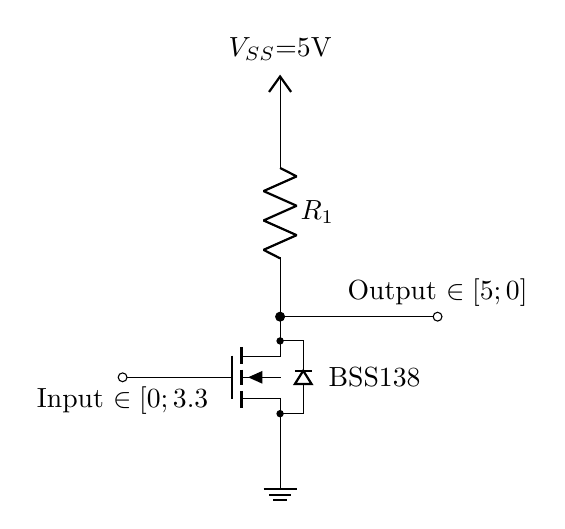
\begin{tikzpicture}[scale=2]
	\draw[color=black]
	(0,-0.5) node[ground]{}
	(0,0) node[nfet,bodydiode](npn){}
	
	(npn.B)+(0.6,0) node[]{BSS138}
	
	(0,1.7) node[vcc]{$V_{SS}$=5V}
	(0,1.7) to [R=$R_1$] (npn.D)
	(npn.S) to (0,-0.5)
	
	(-1,0) node[anchor=north]{Input $\in [0;3.3$}
	to[short,o-] (npn.G)
	
	(npn.D)+(1,0) node[anchor=south]{Output $\in [5;0]$}
	to[short,o-*]  (npn.D)
	
	
	;
	
\end{tikzpicture}

 	\caption{Logic Level Converter \& Inverter Circuit}
 	\label{fig:interterCirc}
 \end{figure}
 
 
 The microcontroller is required to interface with the motor driver and represent a logical high and low as a \SI{3.3}{V} and \SI{0}{V} respectively. The motor driver's logical high threshold is \SI{3.5}{V}. It is thus required to use a logic level converter to allow reliable communication between the two devices.\\
 
 The logic level converter used shown in Figure \ref{fig:interterCirc} uses the BSS128 transistor. The circuit shown also acts as an inverter where a logic low, \SI{0}{V} by the microcontroller will be converted to a \SI{5}{V} and a logic high, \SI{3.3}{V} will be converted to \SI{0}{V}. This side effect was overcome by inverting the desired responses in software.
 
 
 \subsubsection{AND Digital Circuit}
 \begin{figure}[h]
 	\centering
 	% Block Diagram for TTL IC Multiplexer 74HC153
% Author: Ramón Jaramillo.
\documentclass[tikz,border=10pt,12pt,x11names]{standalone}
%%%<
\usepackage{verbatim}
%%%>
\begin{comment}
:Title: Block Diagram for TTL IC Multiplexer 74HC153
:Tags: Circuits;Electrical engineering
:Author: Ramón Jaramillo
:Slug: multiplexer

This image was taken from a handbook about TTL Logic devices.
\end{comment}
\usepackage{tikz}
\usetikzlibrary{circuits.logic.US} % TiKZ Library for US Logic Circuits.
\begin{document}
	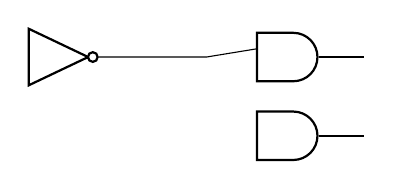
\begin{tikzpicture}[circuit logic US, every circuit symbol/.style={thick}]
	% Logic Gates
	\node[and gate,inputs={nn}, point right] (and1) at (2,-1)    {};
	\node[and gate,inputs={nn}, point right] (and2) at (2,-2)    {};
	\node[not gate, point right]               (not1) at (-1,-1) {};
	
	
	\draw (not1.output) -| (1,-1) -- (and1.input 1);
	
	%Outputs
	\draw (and1.output) [thick]-- (3,-1);
	\draw (and2.output) [thick]-- (3,-2);
	
	
	
	
	
	\end{tikzpicture}
\end{document}
 	\caption{AND Digital Logic with Inverter}
 	\label{fig:andCircuit}
 \end{figure}
 
 \begin{figure}[h]
 	\centering
 	\def\degr{${}^\circ$}
\begin{tikztimingtable}[timing/d/text/.append style={font=\rmfamily}]
  PWM Signal 10\,kHz	   & H 12{2C} G\\
  Direction Signal  	   & L  12L  12H \\
  A						   & L 12L 12H \\
  IN1				   	   & H 6{2C} 12{L}  \\
  IN2			   		   & L 7{2L} 5{2C}  \\
  %Coarse Pulse             & 3L 16H 6L \\
  %Coarse Pulse - Delayed 1 & 4L N(B2) 16H N(B6) 5L \\
  %Coarse Pulse - Delayed 2 & 5L N(B3) 16H N(B7) 4L \\
  %Coarse Pulse - Delayed 3 & 6L 16H 3L \\
  \\
  %Final Pulse Set          & 3L 16H N(B5) 6L \\
  %Final Pulse $\overline{\mbox{Reset}}$ & 6L N(B4) 16H 3L \\
  %Final Pulse              & 3L N(B1) 19H N(B8) 3L \\
\extracode
  \tablerules
  %0\begin{pgfonlayer}{background}
 %   \foreach \n in {1,...,1}
  %    \draw [help lines] (A\n) -- (B\n);
  %\end{pgfonlayer}
\end{tikztimingtable}
 	\caption{AND Digital Logic Circuit Waveforms}
 	\label{fig:andCircuit_waveform}
 \end{figure}
 
 The motor driver contains 2 input pins which controls the voltage polarity of the motor terminals. Keeping the one input high and the other low will turn the motor in the one direction and switching the logical values on these inputs will turn the motor on the other direction. Adding speed control requires the pulse-width-modulated (PWM) signal that the motor receives to be alternated on these inputs and are done by the AND digital circuit.\\
 
 The AND circuit receives 2 signals from the microcontroller  after it has been converted to the correct logic level: the PWM signal and a logic level signal indicating the desired direction. Based on the directional signal the AND circuit will switch the PWM signal between the 2 inputs of the motor driver while holding the other low as seen in Figure \ref{fig:andCircuit_waveform}.\\
 
 This hardware directional control was done in order to reduce the processing time the microcontroller was required to do in order to switch the generated PWM signal between the 2 inputs of the motor driver.

\subsection{Motor Driver}
\begin{figure}[h]
	\centering
	\documentclass[tikz,border=10pt,12pt,x11names]{standalone}
%%%<
\usepackage{verbatim}
%%%>
\usetikzlibrary{calc,arrows}
\usepackage{tikz}
\usepackage[]{circuitikz} % TiKZ Library for US Logic Circuits.
\usetikzlibrary{circuits.logic.US} % TiKZ Library for US Logic Circuits.
\usepackage{amsmath}

\usepackage{tikz}
\usetikzlibrary{circuits.logic.US} % TiKZ Library for US Logic Circuits.
\begin{document}
	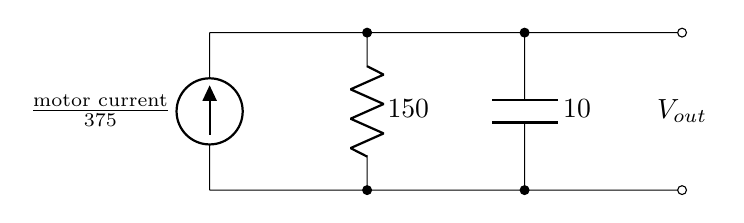
\begin{tikzpicture}[scale=2,american currents]
	
	
	\draw (0,0) to[I,l=$\frac{\textnormal{motor current}}{375}$] (0,1)
	(0,1) to[short,-o] (3,1)
	
	(1,1) to[R=150,*-*] (1,0)
	(0,0) to[short,-o] (3,0)
	
	(2,1) to[C=10 ,*-*] (2,0);
	
	
	\draw (3,0.5) node[]{$V_{out}$};
	
	\end{tikzpicture}
\end{document}
	\caption{Simplified Circuit of Motor Feedback}
	\label{fig:feedback_current}
\end{figure}


The motor driver chosen was the MC33887. It was selected based on providing the motor up to \SI{6}{\ampere} of current, while withstanding the high current transients due to the fast switching of a inductive load \citep{motorIC}. The motor driver provides the motor with 12V DC which is externally provided by a DC power supply. The schematic of the motor driver is shown in Appendix \ref{sec:schematics}.\\

The motor driver is connected directly to the motor and responsible for directional and rotational control of the brushed DC motor. The motor driver contains 2 half H-bridges that forms a full H-bridge which are PWM to control the speed of the motor and originates from the microcontroller. The selected frequency was 10kHz and is recommended by the manufacturers \citep{motorIC}. As discussed previously, the signals' logic level was first converted and then sent through the AND digital filter before the motor driver receives it.\\

The MC33887 provides a proportional current of $\frac{1}{375}$ of the current flowing through the high-side of the full H-bridge \citep{motorIC}. This current is sent through a resistor of \SI{150}{\Omega} to provide a voltage signal to represent the current. Due to the motor being controlled using PWM, the current is a periodic impulse signal making it almost impossible for the ADC to sample. This problem was overcome by adding a parallel capacitor to the resistor to create a ripple voltage. This ripple voltage is sent through an unity-gain amplifier as seen in Figure \ref{fig:unitygain} before it is sampled by the micro-controller. The $R_{\text{input}}$ resistance is the input resistance that the operational amplifier sees. This closes the feedback loop to implement torque control by the control system.\\

\subsection{Verification Tests}

\subsubsection{ PWM Duty Cycle to Motor Current}

\begin{figure}[h]
	\centering
	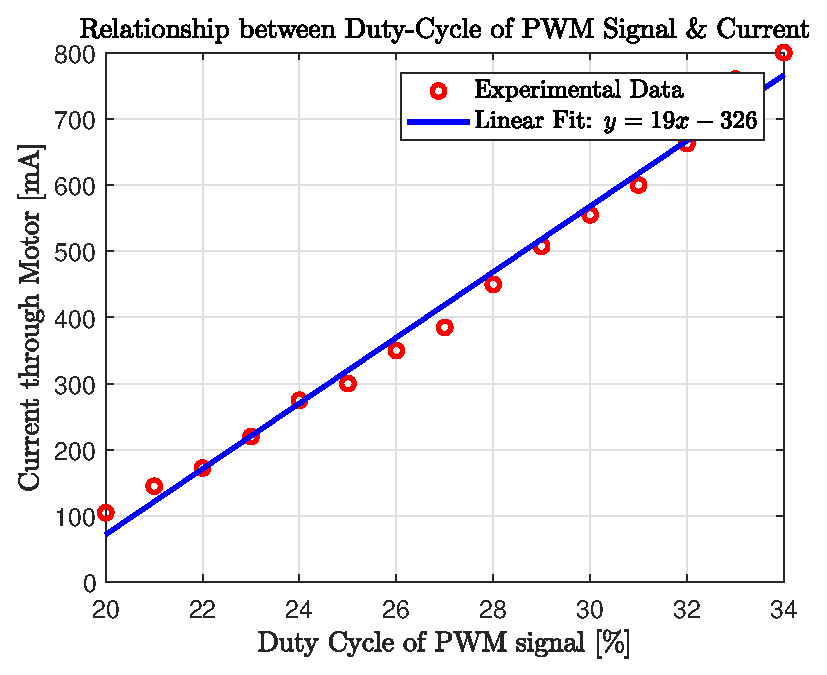
\includegraphics[scale=1]{./figs/dutycycle_vs_current.eps}
	\caption{Relationship between Duty-Cycle of PWM Signal and Current through Motor}
	\label{fig:dutycycle_vs_current}
\end{figure}

The model describing the system in equation (\ref{eq:condense2}) assumes the torque delivered to the system is instantaneously available. This is inaccurate due to the fact that the model describing the DC motor is a second-order differential equation containing its own time constant. This model was not incorporated as adding another control loop would add more delays to the control systems. This was overcome by mapping the torque the motor provided to the duty cycle the motor receives.\\

Experiments were done to determine the relationship between the duty-cycle of the PWM signal and the torque delivered by the motor. These experiments are done by incrementing the duty-cycle of the PWM signal that the motor receives when the shaft is kept fixed against a hard-stop. The mean value of the output voltage from the circuit shown in Figure \ref{fig:feedback_current} was measured on the oscilloscope and mapped backwards to determine the torque using equation (\ref{eq:duty2current}) with the definition of the constants shown in Table \ref{table:duty2current_constants}.
\begin{equation} \label{eq:duty2current}
\tau = \frac{V}{R}\cdot GR \cdot FR \cdot \alpha_{t}
\end{equation}

\begin{table}[]
	\centering
	\begin{tabular}{|c|c|c|}
		\hline
		Constant & Description & Value \\
		\hline
		\hline
		GR &  Gear Ratio & 14 \\
		\hline
		FR & Feedback Current Ratio & 375 \\
		\hline
		$\alpha_{t}$ & Torque Constant & $19.1\times 10^{-3}$ \\
		\hline
		R & Resistance & 150 \\
		\hline
	\end{tabular}
	\caption{Values of Constants used in Equation (\ref{eq:duty2current})}
	\label{table:duty2current_constants}
\end{table}

 Figure \ref{fig:dutycycle_vs_current} shows the measured data with a line of best fit. It is clear that there exists a linear relationship between the duty-cycle of the PWM signal and the torque provided. This equation of best fit will thus be used to output the correct torque determined by the control system.


\chapter{Software Design}
\label{chp5:software}
%WHAT you are going to present in this chapter/section
%WHY you are presenting it, and
%HOW you are going to present it
\section{Software Requirements}
\label{sec:software_requirements}
The software required to implement the retrieval of system state information, debugging and control laws are presented here. The software design played a central role in continuing the project pass the simulation phase. The software design allowed the determination of the system characteristic parameters and the verification of the simulation and controller.

\subsection{Communication}

Communication between the external computer and the microcontroller occurred differently based on whether an experiment was done or testing different parts of the electronic system. These difference are explained in this section.\\

If experiments are conducted the communication are bi-directional between the microcontroller and the external computer. The microcontroller streams the state variables of the system to the external computer in the structure shown in Figure \ref{fig:data_struct}. The star attached to the variables indicate that they are not sent in the correct units due to sending data types such as floats are computation hungry and are rather handled on the external computer. The external computer will then translate the variables into their correct units and compute the control input based on the control law. The external computer sends the control input back to the microcontroller to output the correct signals.\\

\begin{figure}[h]
	\centering
		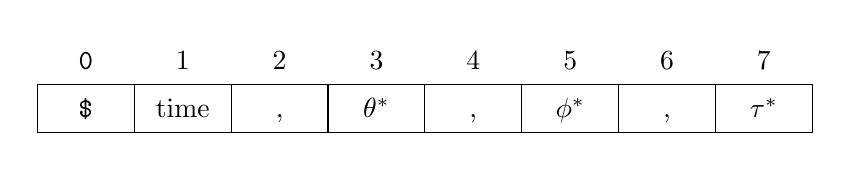
\begin{tikzpicture}[cell/.style={rectangle,draw=black},
	space/.style={minimum height=1.5em,matrix of nodes,row sep=-\pgflinewidth,column sep=-\pgflinewidth,column 1/.style={font=\ttfamily}},text depth=0.5ex,text height=2ex,nodes in empty cells]
	

	
	\matrix (first)[space, row 2/.style={minimum width=3em,nodes={cell,minimum width=3.5em}},row 3/.style={nodes={cell,minimum width=2em}}]
	{
		0   & 1  & 2 & 3 & 4 & 5& 6& 7  \\   
		\$  & time  & , & $\theta^{*}$ &,& $\phi^{*}$ &,& $\tau^{*}$ \\};
	
	
	
	
	\end{tikzpicture}
	\caption{Data Structure for Streaming Data during Experiments}
	\label{fig:data_struct}
\end{figure}

The structure used in Figure \ref{fig:data_struct} was chosen as comma-seperated values (.csv) which makes it easy to write the data in a .csv file to analyse later.\\

The other state in which communication occurred was used for debugging purposes. In this state the \textit{Python} script allows the user to type commands adhering to the structure shown in Figure \ref{fig:uart_struct}. Based on the command used, the microcontroller would echo the same command back if it completed the command instructed. These commands included to receive the sampled values of signals, manual control over the duty-cycle of the PWM signal and directional control of the motor. It also acted as a soft layer for safety by sending commands to arm the system before experiments. A summary of the possible commands are given in Appendix \ref{sec:software_requirements}.


\begin{figure}[h]
	\centering
	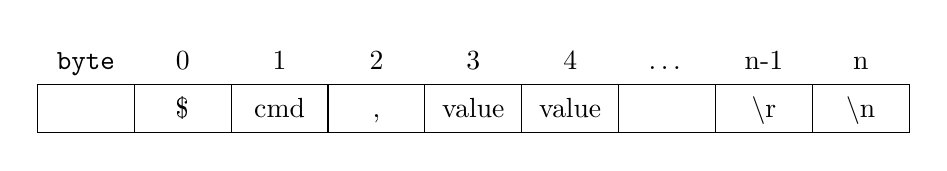
\begin{tikzpicture}[cell/.style={rectangle,draw=black},
	space/.style={minimum height=1.5em,matrix of nodes,row sep=-\pgflinewidth,column sep=-\pgflinewidth,column 1/.style={font=\ttfamily}},text depth=0.5ex,text height=2ex,nodes in empty cells]
	

	
	\matrix (first)[space, row 2/.style={minimum width=3em,nodes={cell,minimum width=3.5em}},row 3/.style={nodes={cell,minimum width=2em}}]
	{
		byte &0   & 1  & 2 & 3 & 4& \ldots & n-1&n  \\   
		&\$  & cmd  & , & value & value &  & \textbackslash r &  \textbackslash n \\};
	
	
	
	
\end{tikzpicture}
	\caption{Data Structure for Sending Commands}
	\label{fig:uart_struct}
\end{figure}


\subsection{Embedded Program}

%\begin{comment}
\begin{figure}[h]
\centering
% Define block styles
\tikzstyle{decision} = [diamond, draw, fill=blue!20, 
    text width=4.5em, text badly centered, node distance=3cm, inner sep=0pt]
\tikzstyle{block} = [rectangle, draw, fill=blue!20, 
    text width=5em, text centered, rounded corners, minimum height=4em]
\tikzstyle{line} = [draw, -latex']
\tikzstyle{cloud} = [draw, ellipse,fill=red!20, node distance=3cm,
    minimum height=2em]
    
\begin{tikzpicture}[node distance = 2cm, auto]
    % Place nodes
    \node [block] (initperip) {Initialise Peripherals};
    \node [block, below of=initperip] (initvars) {Initialise Variables};
    \node [decision, below of=initvars] (uart) {Byte received?};
    \node [decision, below of=uart] (uart) {};
    %\node [block, below of=init_vars] (evaluate) {evaluate candidate models};
    %\node [block, left of=evaluate, node distance=3cm] (update) {update model};
    %\node [decision, below of=evaluate] (decide) {is best candidate better?};
    %\node [block, below of=decide, node distance=3cm] (stop) {stop};
    
    \node [cloud, left of=init_perip] (expert) {expert};
    \node [cloud, right of=init_perip] (system) {system};
    % Draw edges
   \path [line] (initperip) -- (initvars);
  %  \path [line] (identify) -- (evaluate);
  %  \path [line] (evaluate) -- (decide);
  %	\path [line] (uart) -| node [near start] {yes} ();
   % \path [line] (update) |- (identify);
   % \path [line] (decide) -- node {no}(stop);
  %  \path [line,dashed] (expert) -- (init);
  %  \path [line,dashed] (system) -- (init);
  %  \path [line,dashed] (system) |- (evaluate);
\end{tikzpicture}
\caption{Embedded Software Flow}
\label{fig:software_flow}
\end{figure}
%\end{comment}


Figure \ref{fig:software_flow} shows the main execution flow of the microcontroller based on factors that influence their states. A brief overview of the execution flow is described below.\\

On startup of the microcontroller, the various peripherals required for operation are initialised. They include timers for PWM generation, ADC for sampling and interrupts for encoder signals. The microcontroller will then initialise the various variables required for operation.\\

Once initialisation was completed the microcontroller will check via an interrupt if a byte over the serial communication has been received. If a byte has been received, the microncontroller will verify the command structure and execute based on this command.\\

Every 0.1ms the microcontroller will inspect the data arrays of the sampled signals. Direct Memory Access (DMA) was used for sampling and results in the sampled data to be automatically refreshed by hardware.\\

The microcontroller will then react whether a interrupt has occured to indicate a rising or falling edge on the encoder signal. This falling and rising edge indicates a incremental change of the position of the actuated pendulum and the microcontroller will behave accordingly.\\

The microcontroller will than verify whether it is required to stream the data every 4ms to the external computer for system identification tests.\\

\subsection{Controller}
%WHAT you are going to present in this chapter/section
%WHY you are presenting it, and
%HOW you are going to present it
The controllers of the swing-up and balancing are implemented on the external computer in a \textit{Python} script and required more information about the system state than what was received from the microcontroller. How these missing information was determined is explained in this section.\\

The information the swing-up and balancing controllers required was the angular velocity of both the actuated and unactuated pendulum. This information was acquired using numerical differentiation by using the 3-point backwards method shown in equation (\ref{eq:differentiation}).

\begin{equation} \label{eq:differentiation}
f'(x) \approx \frac{-3f(x)  +  4f(x-{\Delta}t)  -  f(x-2{\Delta}t)}{ 2{\Delta}t }
\end{equation}

The swing-up controller implements multiple cosine and sine functions. These functions were discretised into a lookup table up to the accuracy provided by the sensors. The discretisation was done to decrease the processing time done to compute the next control input command.



\chapter{Practical Results}
\label{chp:prac_results}
%WHAT you are going to present in this chapter/section
%WHY you are presenting it, and
%HOW you are going to present it






\section{Swingup Controller}
%WHAT you are going to present in this chapter/section
%WHY you are presenting it, and
%HOW you are going to present it
This section provides the practical results of the swing-up controller and discusses the differences it contains with the simulation. \\

Figure \ref{fig:experiment_swingup} shows the practical results of the swing-up controller and contains interesting behaviour that the simulation does not contain. The swing-up controller did not require a initial condition as in the simulation. The system started to swing-up from the rest position because of the noise being introduced by the ADC. This noise is amplified by using the numerical differential algorithm to calculate the angular velocity of the pendulums that is required by the swing-up controller. The swing-up controller reacts on this small error which results in the motor to output a torque and provides this small initial condition.\\




\section{Balancing Controller}
%WHAT you are going to present in this chapter/section
%WHY you are presenting it, and
%HOW you are going to present it
\section{Swingup and Balancing}
%WHAT you are going to present in this chapter/section
%WHY you are presenting it, and
%HOW you are going to present it
\chapter{Conclusion}
\label{chp:conclusion}



\section{Summary}
%WHAT you are going to present in this chapter/section
%WHY you are presenting it, and
%HOW you are going to present it
A feedback control system was designed, implemented and verified in simulation to swing and balance a robotic gymnast. The feedback control system met all requirements and was able to swing the robotic gymnast from the hanging position and balance in the inverted position.\\
 
The mechanical and electronic hardware were designed to create a robotic gymnast system on which these feedback control systems can be tested. The designed electronic hardware was able to condition the signals for a microcontroller to interpret and supply the feedback control system with the correct signals. The electronic hardware provided good resolution of the required state variables and capable of communicating with all peripherals. The mechanical hardware successfully interfaced with the electronic hardware and provide the means to practically test the feedback control laws.\\

Furthermore the characteristic of the robotic gymnast system was identified and used in simulation. The simulation was shown as a good representation of the designed robotic system to allow further developments on the simulated model. The simulated model fits the experimental responses well and contain the characteristics determined during the system identification.\\

Software was written to acquire the data during experiments and communicate with the electronic hardware. The software allows for various modes of communication such as debugging of subcircuits and streaming of data.\\

\section{Recommendation}
%WHAT you are going to present in this chapter/section
%WHY you are presenting it, and
%HOW you are going to present it
A short description of the improvements that can be made with regards to \textit{The Feedback Control Of A Robotic Gymnast} is provided in this section, in an attempt to improve the quality of future research.\\

Choosing a more advanced microcontroller that is able to use a baudrate greater than 115200 would improve response time and provide better control of the system.\\

Implementing a digital low pass filter to remove the noise on the sampled signal. Especially on the signals that are required to be numerically differentiated.\\

The script executing on the external computer can be written in a language such as C or C++ to increase the execution time of the script.\\


\newpage

	
%==== Appendices ====================================================
\appendix
\appendixpage\relax

\chapter{}
\begin{comment}
An outcome assessment must accompany the Final Report and included and bound into the
report after the summary page. This assessment is a single page on which the student must
indicate which parts of the report presents evidence of achieving each of the ECSA outcomes
(as specified in this document). A sentence or two can also be given for each outcome to
explain how those parts of the report demonstrate achieving the outcome
\end{comment}

\label{chp2:concept_model}

\section{Derivation of the Mathematical Model}
\label{sec:math_model}

$$x_{1}= l_{1}\cos(\theta)$$
$$y_{1} = -l_{1}\sin(\theta)$$

$$x_{2} = L_{1}\sin(\theta) + l_{2}\sin(\theta + \phi)$$
$$y_{2} = -L_{1}\cos(\theta) - l_{2}\cos(\theta + \phi)$$

$$\dot{x_{2}} = L_{1}\cos(\theta)\dot{\theta} - l_{2}\cos(\theta+\phi)(\dot{\theta}+\dot{\phi}) $$
$$\dot{y_{2}} = L_{1}\sin(\theta)\dot{\theta}+l_{2}\sin(\theta+\phi)(\dot{\theta}+\dot{\phi})$$

$$x_{2}^2 = L_{1}^2\cos(\theta)^2\theta^2 +l_{2}^2\cos(\theta+\phi)^2(\dot{\theta}+\dot{\phi})^2 + 2L_{1}l_{2}\dot{\theta}(\dot{\theta}+\dot{\theta})\cos(\theta)\cos(\theta+\phi)$$
$$y_{2}^2 = L_{1}^2\sin(\theta)^2\theta^2 +l_{2}^2\sin(\theta+\phi)^2(\dot{\theta}+\dot{\phi})^2 + 2L_{1}l_{2}\dot{\theta}(\dot{\theta}+\dot{\theta})\sin(\theta)\sin(\theta+\phi)$$

$$x_{2}^2+y_{2}^2 = L_{1}^2\theta^2[\cos(\theta)^2+\sin(\theta)^2]+l_{2}^2(\dot{\theta}+\dot{\phi})^2[\cos(\theta+\phi)^2+\sin(\theta+\phi)^2] +$$
$$ 2L_{1}l_{2}\dot{\theta}(\dot{\theta}+\dot{\phi})[\cos(\theta)\cos(\theta+\phi)+\sin(\theta)\sin(\theta+\phi)]$$	

Using the following trigonometric identities $$ \cos(\gamma)^2 + \sin(\gamma)^2 = 1 $$ 
$$ \cos(\gamma)\cos(\alpha)+\sin(\gamma)\sin(\alpha) = \cos(\gamma - \alpha) $$ the above equation resolves to: $$ V_{2}^2 = L_{1}\dot{\theta}^2+l_{2}^2(\dot{\theta}+\dot{\phi})^2 + 
2L_{1}l_{2}(\dot{\theta}+\dot{\phi})\dot{\theta}\cos(\phi)$$

The kinetic energy in the system consist of the fixed rotation of the underactuated  pendulum and the rotation and velocity of the actuated pendulum.

$$ T = \frac{1}{2}I_{A}\dot{\theta}^2 + \frac{1}{2}I_{B}(\dot{\theta}+\dot{\phi})^2 + \frac{1}{2}m_{2}V_{2}^2$$
$$ T = \frac{1}{2}I_{A}\dot{\theta}^2 + \frac{1}{2}I_{B}(\dot{\theta}+\dot{\phi})^2 + \frac{1}{2}m_{2}[L_{1}\dot{\theta}^2+l_{2}^2(\dot{\theta}+\dot{\phi})^2 + 
2L_{1}l_{2}(\dot{\theta}+\dot{\phi})\dot{\theta}\cos(\phi)]^2$$

The potential energy in the system is defined as
$$V=-m_{1}gl_{1}\cos(\theta)-m_{2}g[L_{1}\cos(\theta)+l_{2}\cos(\theta+\phi)]$$

The Lagrange is defined as 
$$\mathcal{L}=T-V$$
$$\mathcal{L} = \frac{1}{2}I_{A}\dot{\theta}^2 + \frac{1}{2}I_{B}(\dot{\theta}+\dot{\phi})^2 + \frac{1}{2}m_{2}[L_{1}\dot{\theta}^2+l_{2}^2(\dot{\theta}+\dot{\phi})^2 + 
2L_{1}l_{2}(\dot{\theta}+\dot{\phi})\dot{\theta}\cos(\phi)]^2+m_{1}gl_{1}\cos(\theta)+$$
$$m_{2}g[L_{1}\cos(\theta)+l_{2}\cos(\theta+\phi)]$$

$$\frac{\partial\mathcal{L}}{\partial\theta} = -m_{1}gl_{1}\sin(\theta)-m_{2}gL_{2}\sin(\theta)-m_{2}gl_{2}\sin(\theta+\phi)$$
$$\frac{d}{dt}\frac{\partial\mathcal{L}}{\partial\dot{\theta}} = I_{A}\ddot{\theta}+I_{B}\ddot{\theta}+I_{B}\ddot{\phi}+m_{2}L_{1}^2\ddot{\theta}+m_{2}l_{2}^2\ddot{\theta}+m_{2}l_{2}\ddot{\phi}+2m_{2}L_{1}l{2}\ddot{\theta}\cos(\phi)-2m_{2}L_{1}l_{2}\dot{\theta}\dot{\phi}\sin(\phi)+$$
$$m_{2}L_{1}l_{2}\ddot{\phi}\cos(\phi)-m_{2}L_{1}l_{2}\dot{\phi}^2\sin(\phi)$$


$$\frac{\partial\mathcal{L}}{\partial\phi} = -m_{2}L_{1}l_{2}(\dot{\theta}+\dot{\phi})\dot{\theta}\sin(\phi)-m_{2}gl_{2}\sin(\theta+\phi)$$

$$\frac{d}{dt}\frac{\partial\mathcal{L}}{\partial\dot{\phi}}=I_{B}\ddot{\theta}+I_{B}\ddot{\phi}+m_{2}l_{2}^2\ddot{\theta}+m_{2}l_{2}^2\ddot{\phi}+m_{2}L_{1}l_{2}\ddot{\theta}\cos(\phi)-m_{2}L_{1}l_{2}\dot{\theta}\dot{\phi}\sin(\phi)$$

The differential equation describing the dynamics of the system is
$$\frac{d}{dt}\frac{\partial\mathcal{L}}{\partial\vec{\dot{q}}}-\frac{\partial\mathcal{L}}{\partial q} = B(\dot{q})+\tau(q)$$ 
where  $ q = 
\begin{bmatrix}
\theta \\
\phi
\end{bmatrix}
$
\section{Collocated Linearisation}
\begin{equation} \label{app:eq:condense1}
d_{11}\ddot{\theta}+d_{12}\ddot{\phi} + h_{1} + \psi_{1} = 0
\end{equation}
\begin{equation} \label{app:eq:condense2}
d_{21}\ddot{\theta} + d_{22}\ddot{\phi} + h_{2} + \psi_{2} = \tau
\end{equation}

Starting from the condense equation (\ref{app:eq:condense1}) and (\ref{app:eq:condense2}), $\ddot{q_{1}}$ is solved in equation (\ref{app:eq:condense1}) and substituted in (\ref{app:eq:condense1}) resulting in 

\begin{equation} \label{app:eq:condense2}
\bar{d_{2}}\ddot{\theta} + \bar{h_{2}} + \bar{\psi_{2}} = \tau
\end{equation}
where the newly defined terms are given as: 
$$\bar{d_{2}} = d_{22} - \frac{d_{21}d_{12}}{d_{11}}$$
$$\bar{h_{2}} = h_{2} - \frac{d_{21}h_{1}}{d_{11}} $$
$$\bar{\psi_{2}} = \psi_{2} - \frac{d_{21}\psi_{1}}{d_{11}} $$


$\tau$ can now chosen to linearise the terms in equation (\ref{app:eq:condense2}) as:

$\tau = \bar{d_{2}}v_{2}+\bar{h_{2}} + \bar{\psi}$


\section{Taylor Series Expansion Around Unstable Equilibrium Position}
\label{sec:linerisation}



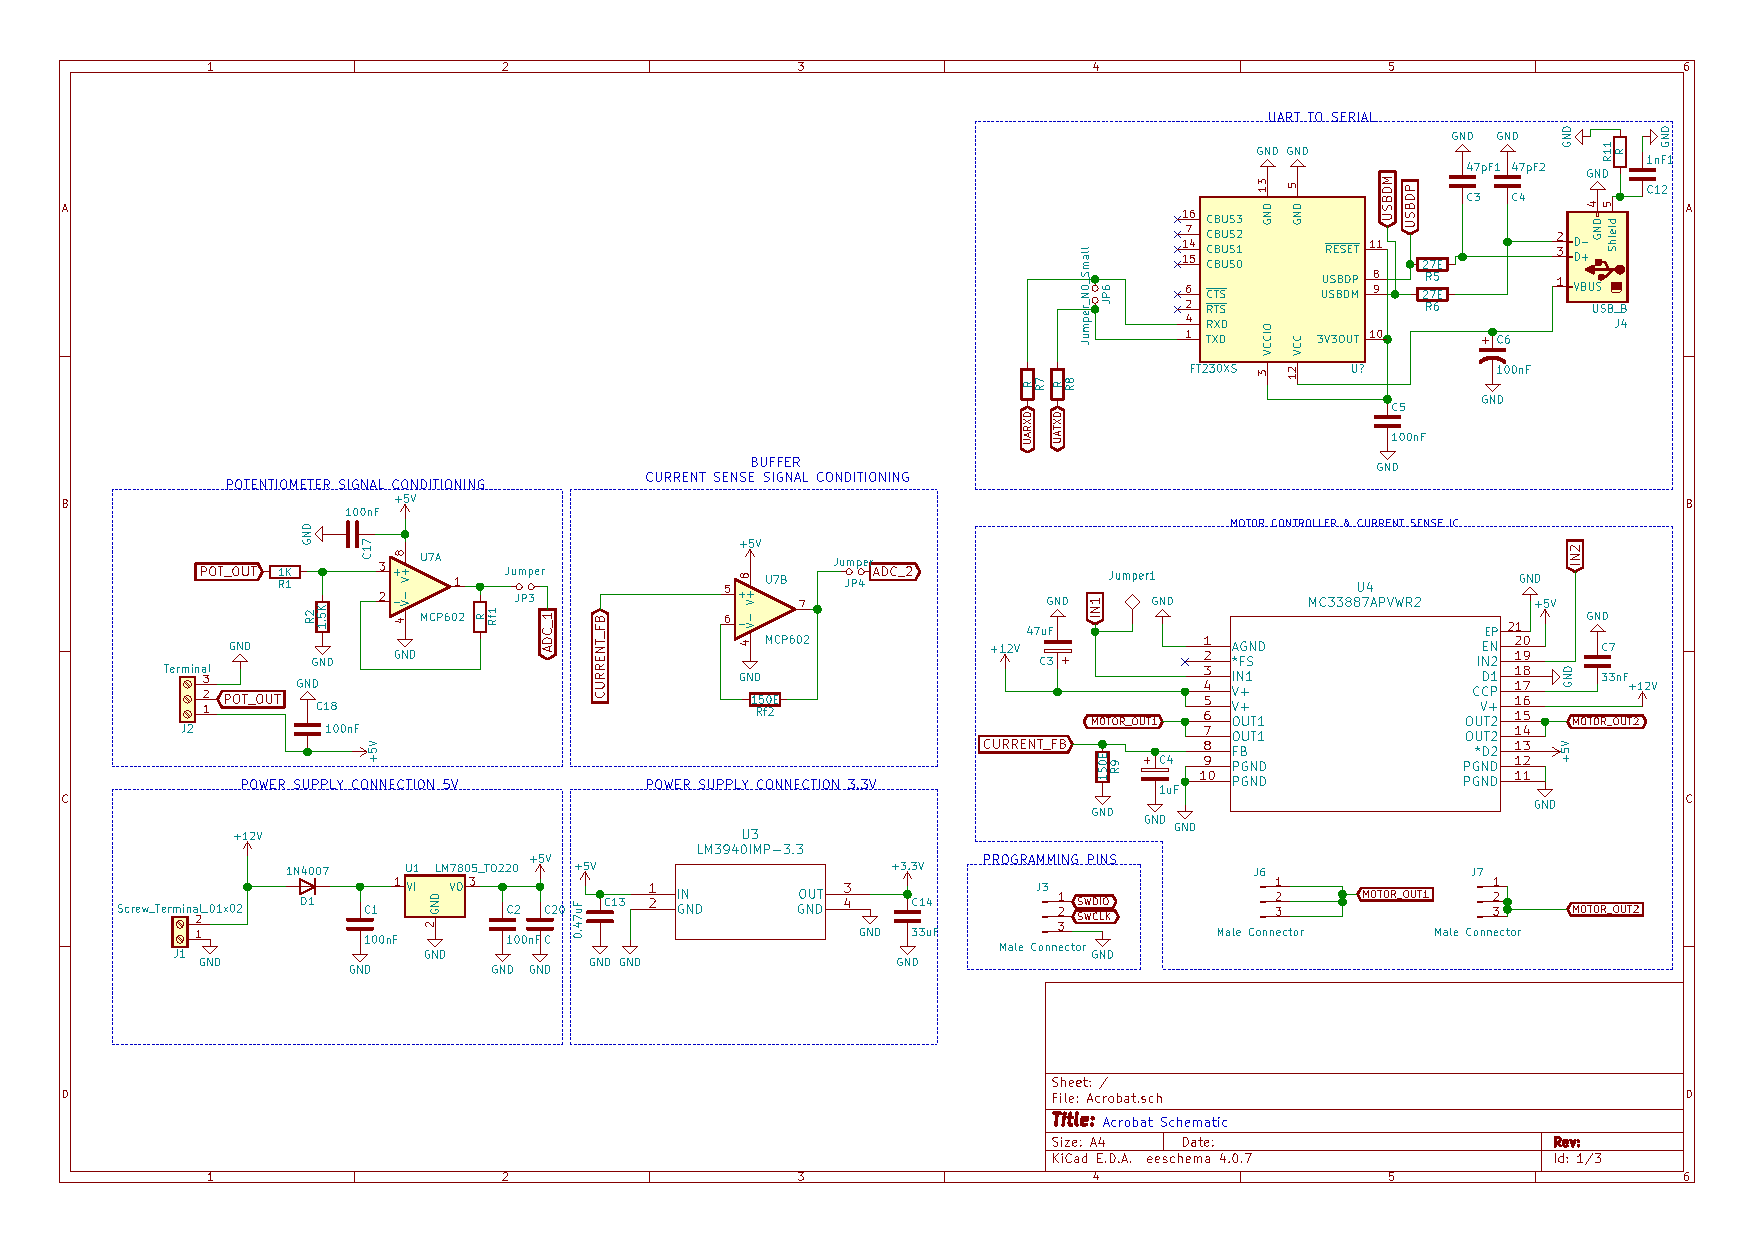
\includepdf[pages=1,pagecommand={\section{Electronic Design Schematic} \thispagestyle{empty} \label{sec:schematics}}, fitpaper=true]{./figs/Acrobat.pdf}
\includepdf[pages=2-,pagecommand={\thispagestyle{empty}}, fitpaper=true]{./figs/Acrobat.pdf}


\section{Communication Structure}
\label{sec:software_requirements}
\begin{figure}[h]
	\centering
	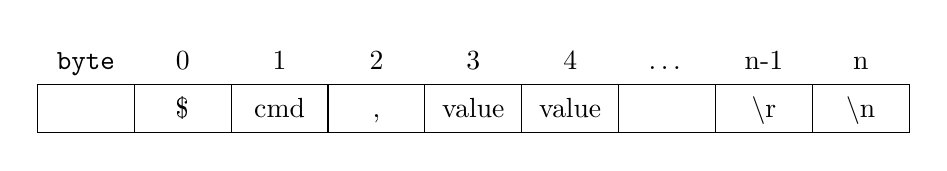
\begin{tikzpicture}[cell/.style={rectangle,draw=black},
	space/.style={minimum height=1.5em,matrix of nodes,row sep=-\pgflinewidth,column sep=-\pgflinewidth,column 1/.style={font=\ttfamily}},text depth=0.5ex,text height=2ex,nodes in empty cells]
	

	
	\matrix (first)[space, row 2/.style={minimum width=3em,nodes={cell,minimum width=3.5em}},row 3/.style={nodes={cell,minimum width=2em}}]
	{
		byte &0   & 1  & 2 & 3 & 4& \ldots & n-1&n  \\   
		&\$  & cmd  & , & value & value &  & \textbackslash r &  \textbackslash n \\};
	
	
	
	
\end{tikzpicture}
	\caption{Data Structure for Sending Commands}
	\label{fig:uart_struct_app}
\end{figure}

In Table \ref{table:uart_commands} the various commmands that are used in the command structure shown in Figure \ref{fig:uart_struct_app} used for debugging purposes is explained with the possible value ranges that can be used.


\begin{table}[h]
	\centering
	\begin{tabular}{|c|c|c|c|}
		\hline
		Command & Range &  Reason for Implementation & Effect \\
		\hline
		\hline
		A & None & Testing of the UART circuit & Send the following text: Feedback Control Of Robotic Gymnast\\
		\hline
		B & 0-100 &  & Changes PWM Duty-Cycle \\
		\hline
		C & 0-1 & Testing of AND digital Circuit Directional Control of Motor & Change the rotational direction \\
		\hline
		D & & & \\
		\hline
	
	\end{tabular}
	\caption{Summary of Communication Commands and their Effects}
	\label{table:uart_commands}

\end{table}


\newpage


%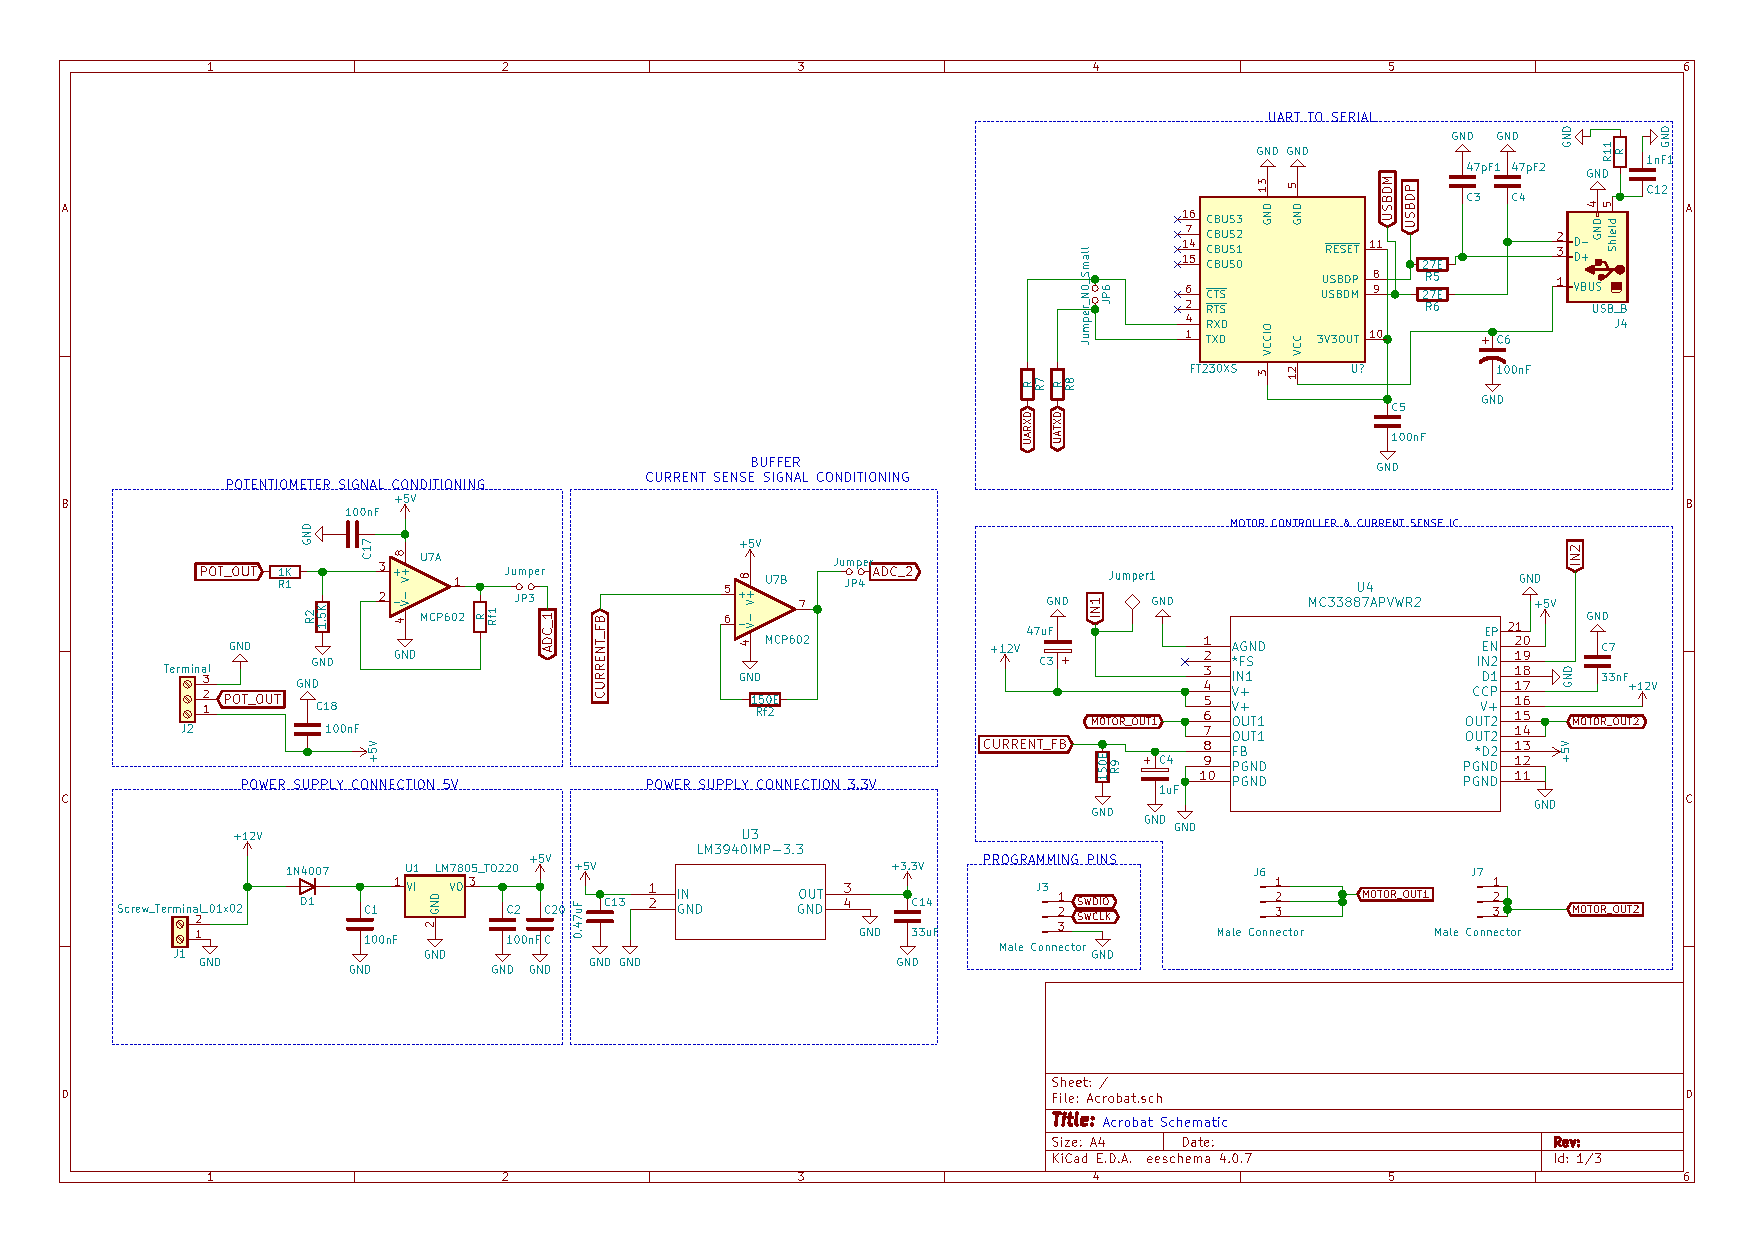
\includepdf[pages=-,scale-=0.8]{./figs/Acrobat.pdf}
%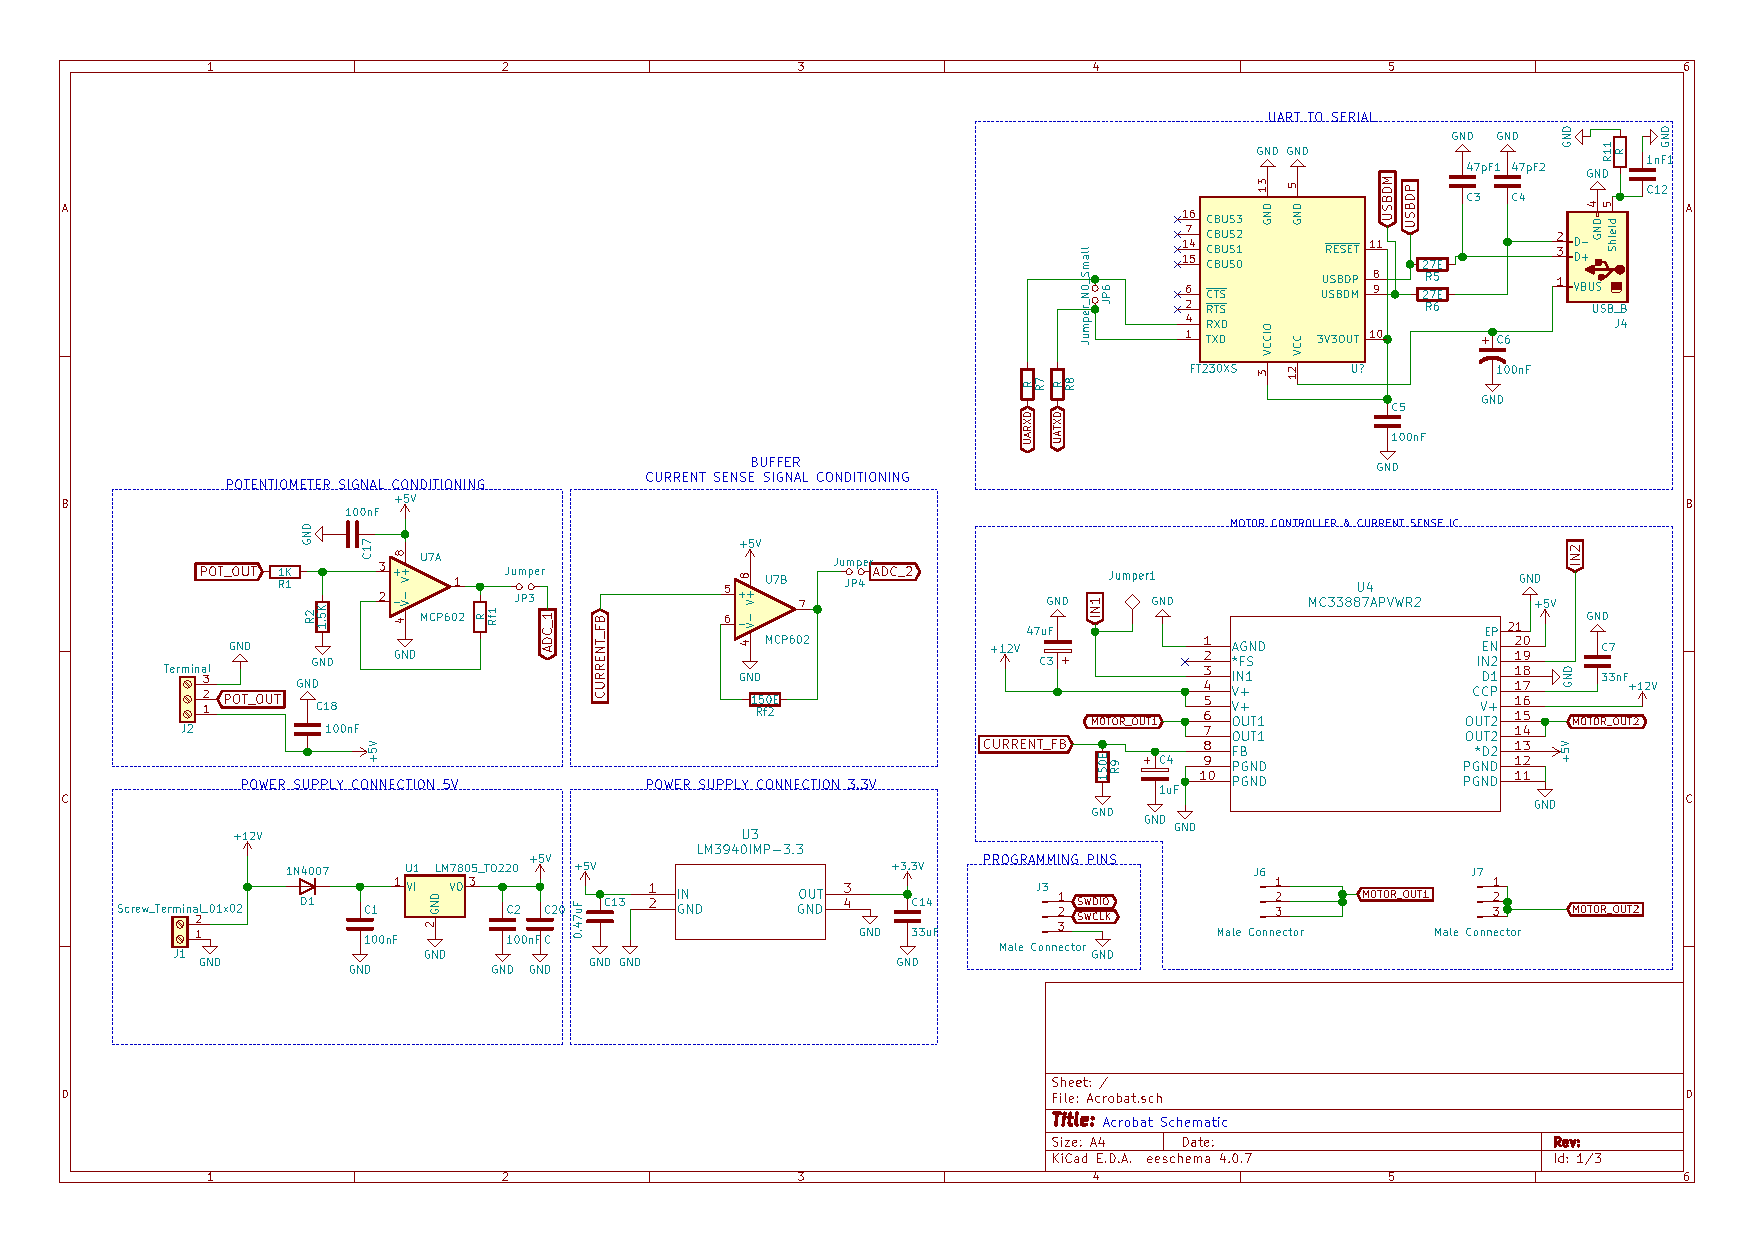
\includegraphics{./figs/Acrobat.pdf}





\section{Techno-Economy Assessment}
\label{sec:techno_eco}

\subsection{Budget}
The comparison between the proposed and actual budget is discussed and why the project was under-budget.\\

The proposed budget for the project was R3000. This budget was required to cover manufacturing cost and the buying of sensors, equipment and components. Table \ref{table:budget} provides the categories and amount of what the project consisted out of.\\

\begin{table}[h]
	\centering
	\begin{tabular}{|c|c|}
		\hline
		Category & Cost \\
		\hline
		\hline
		Electronic Components & R100 \\
		\hline
		Mechanical Components & R300 \\
		\hline 
		Software & R0 \\
		\hline
		Mechanical Manufacturing & R0 \\
		\hline
		Electronical Manufacturing & R0 \\
		\hline
		\hline 
		Total & R200 \\
		\hline
		
	\end{tabular}
	\caption{Categories of the Budget }
	\label{table:budget}
	
\end{table}

It is visible from the budget that the project is under-budget. The reason for being under-budget is due the Electrical and Electronic (E\&E) Deparment providing the service and components which were most expensive. This includes the manufacturing cost of the mechanical and electronic design and the Mechanical and Mechatronic Department providing the most expensive mechanical component.


\subsection{Planning}

\begin{figure}[h]
	\centering
	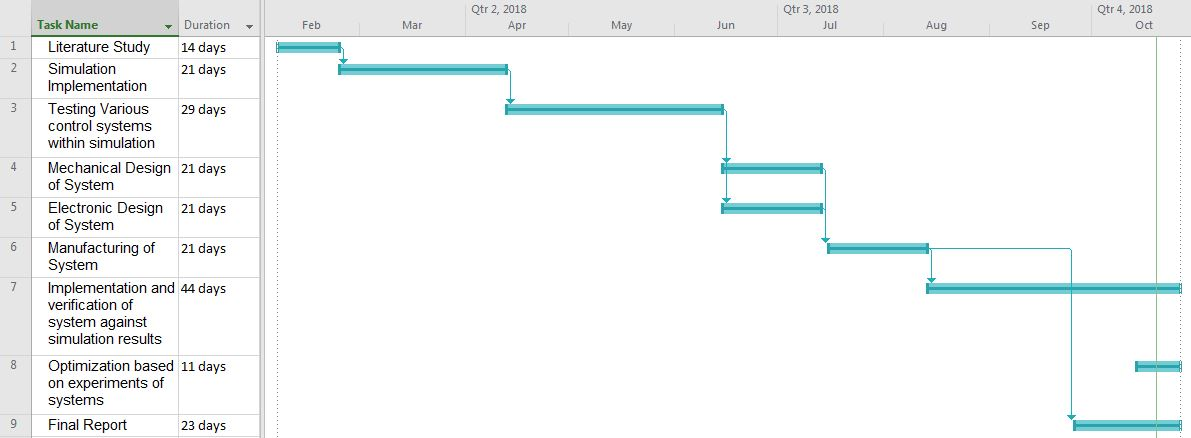
\includegraphics[scale=0.5]{./figs/planning_gantt/ganttchart.jpg}
	\caption{Planned Gantt Chart of the Project}
	\label{fig:planned_ganttchart}
\end{figure}

\begin{figure}[h]
	\centering
	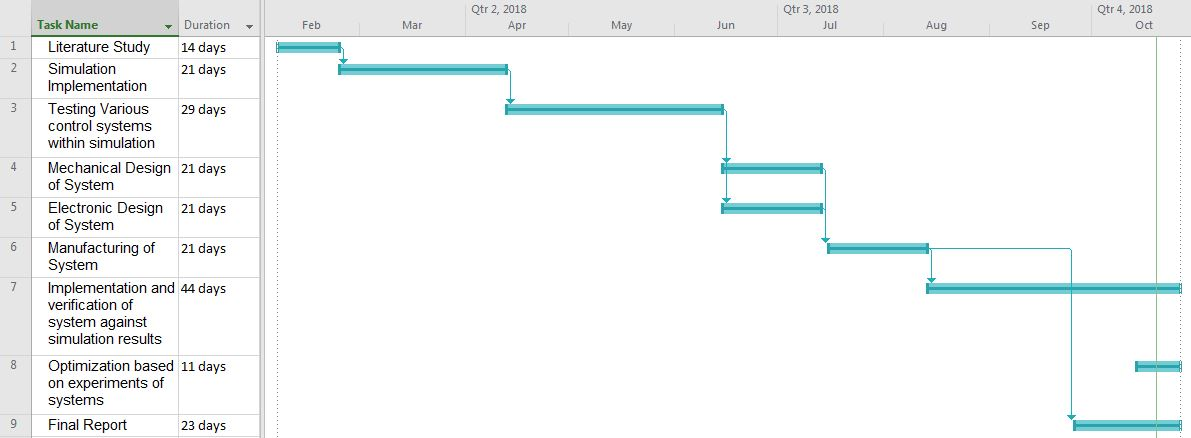
\includegraphics[scale=0.5]{./figs/planning_gantt/ganttchart.jpg}
	\caption{Actual Gantt Chart of the Project}
	\label{fig:actual_ganttchart}
\end{figure}

\begin{table}[h]
	\centering
	\begin{tabular}{|c|c|c|}
		\hline
		Category & Planned Hours & Actual Hours \\
		\hline
		\hline
		Simulation Implementation & 2 & 2 \\
		\hline
		Testing \& Verification of Simulation & 2 & 2 \\
		\hline 
		Mechanical Design  & 2 & 2 \\
		\hline
		Electronic Design & 2 & 2 \\
		\hline
		System Identification Test & 2 & 2 \\
		\hline
		Experiments & 2 & \\
		\hline
		Writing of Report & 2 & 2 \\
		\hline
		
	\end{tabular}
	\caption{Hours worked during the different phases of the project}
	\label{table:hours_worked}
	
\end{table}

Figure \ref{fig:planned_ganttchart} shows the Gantt chart for the planned activities during the project. For the majority of the project, the planned activities were followed as planned. All the activities from the literature study up to the implementation and verification of system results to simulation results.\\

During the experimental phase changes were required to the mechanical design which included a better connection between the motor shaft and actuated pendulum resulting in additional time required for the experiments. This additional time increased the safety during experiments and allowed the practical results presented in the report. This additional time was justified by using the time waiting for the part to be manufacture to write on my report.\\	

The electronic design took longer than what was planned due to experiencing difficulty programming the theoretical controllers on the microcontroller. It was decided to extend the time required for this phase due to without the controllers no practical results of these controllers would be acquired. It was decided to take an additional week to implement the controllers.\\

\subsection{Technical Impact}
The impact of the results presented in this report on the field of control systems, society and industry are discussed and whether the financial input was worthwhile.\\

The problem of the swinging and balancing of the robotic gymnast is a well research problem. Solutions to the swinging and balancing are provided on a theoretical level and supported by simulation results however little practical results are available of these theoretical solutions. The impact of this report includes the practical results of one of these theoretical implementation and discuss how the practical results differ from the theoretical results.\\

The impact of the practical results of this report on the industry of underactuated robotics are little. The robotic gymnast is a interesting problem and consist out of a highly non-linear and linear behaviour and is rather consider a great introductory problem to the field of underactuated robotics.\\

The impact of this report has little impact on society due to being of little interest on industry. The industry will not use the results and discussion presented in this report due to the reasons mentioned in the previous paragraph.\\

The financial input was worthwhile due to providing practical results on one theoretical implementation to the swinging and balancing of the robotic gymnast. \\


\subsection{Return on Investment}
The short and long term value from a technical and economical perspective is provided in this section. A motivation on the continuing research in the field of underactuated robotics are given and the financial cost to further research in this field.\\

Researching underactuated robotics is a exciting and growing research field due to the field of underactuated robotics have increasingly become more important due to technology growing in areas where control is crucial. Areas include: air drones, underwater inspection vehicles, space exploration and the aeroplane industry. \\

Underactuated robotics is an interesting and open field in control, with many design options to approach these types of problems. The most interesting examples of underactuated control problems are legged, swimming and flying robots that has been mentioned in the previous paragraph. This results in underactuated robotics being relevant in many fields.\\

The economical value of underactuated robotics in the short term and long term is high. Products are being brought to market that solve very difficult problems and can be used a broad variety. These products include \textit{Spot} from \textit{Boston Dynamics} which can be used for inspection, transportation and entertainment.\\

The financial cost to further the research on underactuated robotics are low due to the use of simulation programs that allows the testing of solutions on realistic simulated models. This significantly reduce the number of prototypes required to test the solution practically. 

\subsection{Potential for Commercialisation}\
The potential for the commercialisation of the contents within the report is discussed and the value of this commercialisations is given.\\

The contents does not have any real value for commercialisation. As mentioned earlier the problem researched is a very good introductory to underactuated robotics due to containing techniques that is a foundation for more advanced problems. 

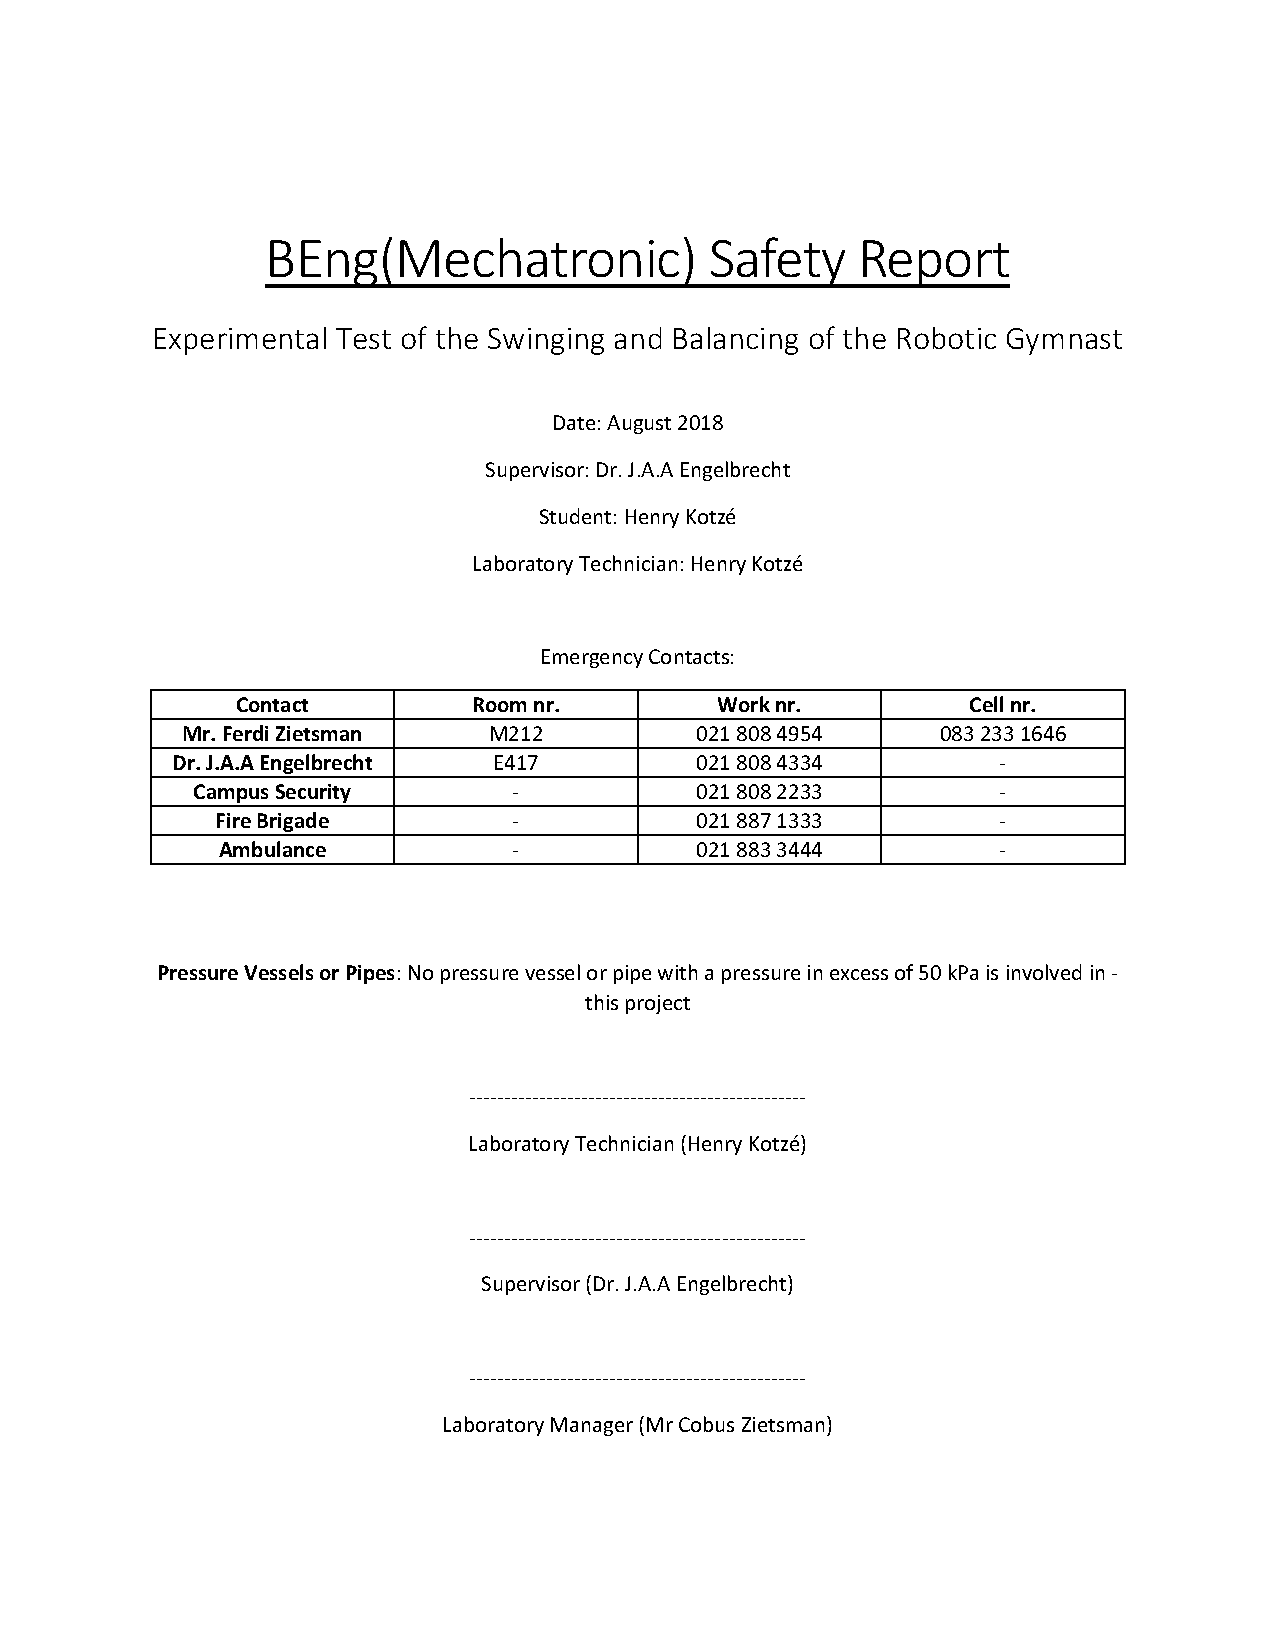
\includepdf[pages=1,pagecommand={\section{Risk Analysis \& Safety Procedures} \thispagestyle{empty} \label{sec:mech_drawings}}, fitpaper=true]{./figs/safety_report/safety_report.pdf}
\includepdf[pages=2-,pagecommand={\thispagestyle{empty}}, fitpaper=true]{./figs/safety_report/safety_report.pdf}

%----------------------------------------------------------------------------
\endinput

%\chapter{Feedback Control Design}
\label{chp:control}


\subsection{Feedback Linearisation}
\label{sec:colocated_linearisation}
%\include{contents/App-3}

%==== Bibliography acro's & Index ===================================
\backmatter

\bibliography{backmatter/USbib-sample}

\end{document}
